% Ross Ice Shelf bathymetry inversion

\section*{Abstract}

Antarctica's Ross Ice Shelf buttresses large catchments of ice from both the East and West Antarctic Ice Sheets. Changes to the current stability of the ice shelf, likely through basal melt of the sensitive grounding zones or pinning points, will reduce this buttressing and accelerate the Antarctic Ice Sheet's contribution to global sea level rise. The distribution of basal melt is predominantly controlled by the ocean cavity thickness and the channelling of ocean waters by bathymetric features. Bathymetry is, however, poorly known for the Ross Ice Shelf. Here we use airborne gravity data and distributed seismic constraints across the ice shelf to create an updated sub-ice shelf bathymetry model. We accomplish this with a non-linear geometric gravity inversion, available as open-source Python code. Monte Carlo sampling of the inversion inputs provides a robust means of addressing spatial uncertainty and the relative significance of each component of the inversion. The resulting bathymetry closely matches the seismic constraints and reveals significant changes compared to past bathymetry models. We find several likely locations of past pinning points, locations where enhanced basal melting is likely, and sites of possible tectonic significance.


\section*{Plain Language Summary}

The floating Ross Ice Shelf slows the flow of a large amount of ice into the ocean. Melting at the base impacts the ice shelf's ability to slow down this upstream ice. The shape of the seafloor beneath the ice shelf (bathymetry), acts to guide ocean currents which cause this melting. Our knowledge of the bathymetry beneath the Ross Ice Shelf comes from a series of point measurements with an average distance between points of over 40~km. Here, we use measurements of Earth's gravity collected over the ice shelf to estimate the shape of the bathymetry beneath. This technique provides an increased resolution of the bathymetry and informs us about where we are most and least confident of the bathymetry depth. With this new model of sub-ice-shelf bathymetry, we highlight locations where melt-inducing ocean currents are likely directed, and several places with the seafloor is very close to the base of the ice. These results will better inform ocean circulation models beneath the ice shelf, and therefore the likely future contributions of the Ross Ice Shelf to sea level rise.


\paragraph*{Key Points}
\begin{enumerate}
    \item We present a new bathymetry model beneath Antarctica's Ross Ice Shelf from a gravity inversion.
    \item A Monte Carlo simulation provides a detailed spatial uncertainty analysis.
    \item Results highlight locations where the updated bathymetry may impact ocean circulation models or where the shelf may have been recently grounded.
\end{enumerate}


\section{Introduction}

Much of Antarctica's coastline is fringed by floating extensions of the Antarctic Ice Sheet. These floating masses of ice, referred to as ice shelves, are connected to the grounded ice on the continent. Over 80\% of Antarctica's grounded ice drains to the oceans through these ice shelves \citep{rignoticeshelf2013}. While they are floating, and thus already displace their mass equivalent of seawater, they are vital to the current and future contribution of the Antarctic Ice Sheet to global sea level rise \citep{fürstsafety2016, jacobsmelting1992}. The ice shelves slow the flow of upstream ice into the ocean by imparting a resistive force, known as buttressing. This buttressing occurs from lateral drag along the sides of the ice shelves and resistive stresses incurred where they flow over pinning points (localized areas of grounded ice) \citep{dupontassessment2005, matsuokaantarctic2015}. Changes to the geometry of the ice shelves can reduce their restraining effect on the flow of grounded ice, leading to an increased mass flux of ice across the grounding zone, thus increasing the ice sheet's contribution to global sea level rise \citep[e.g.,][]{scambosglacier2004, pritchardantarctic2012}. \\

\begin{figure}[!ht]
    \centering
    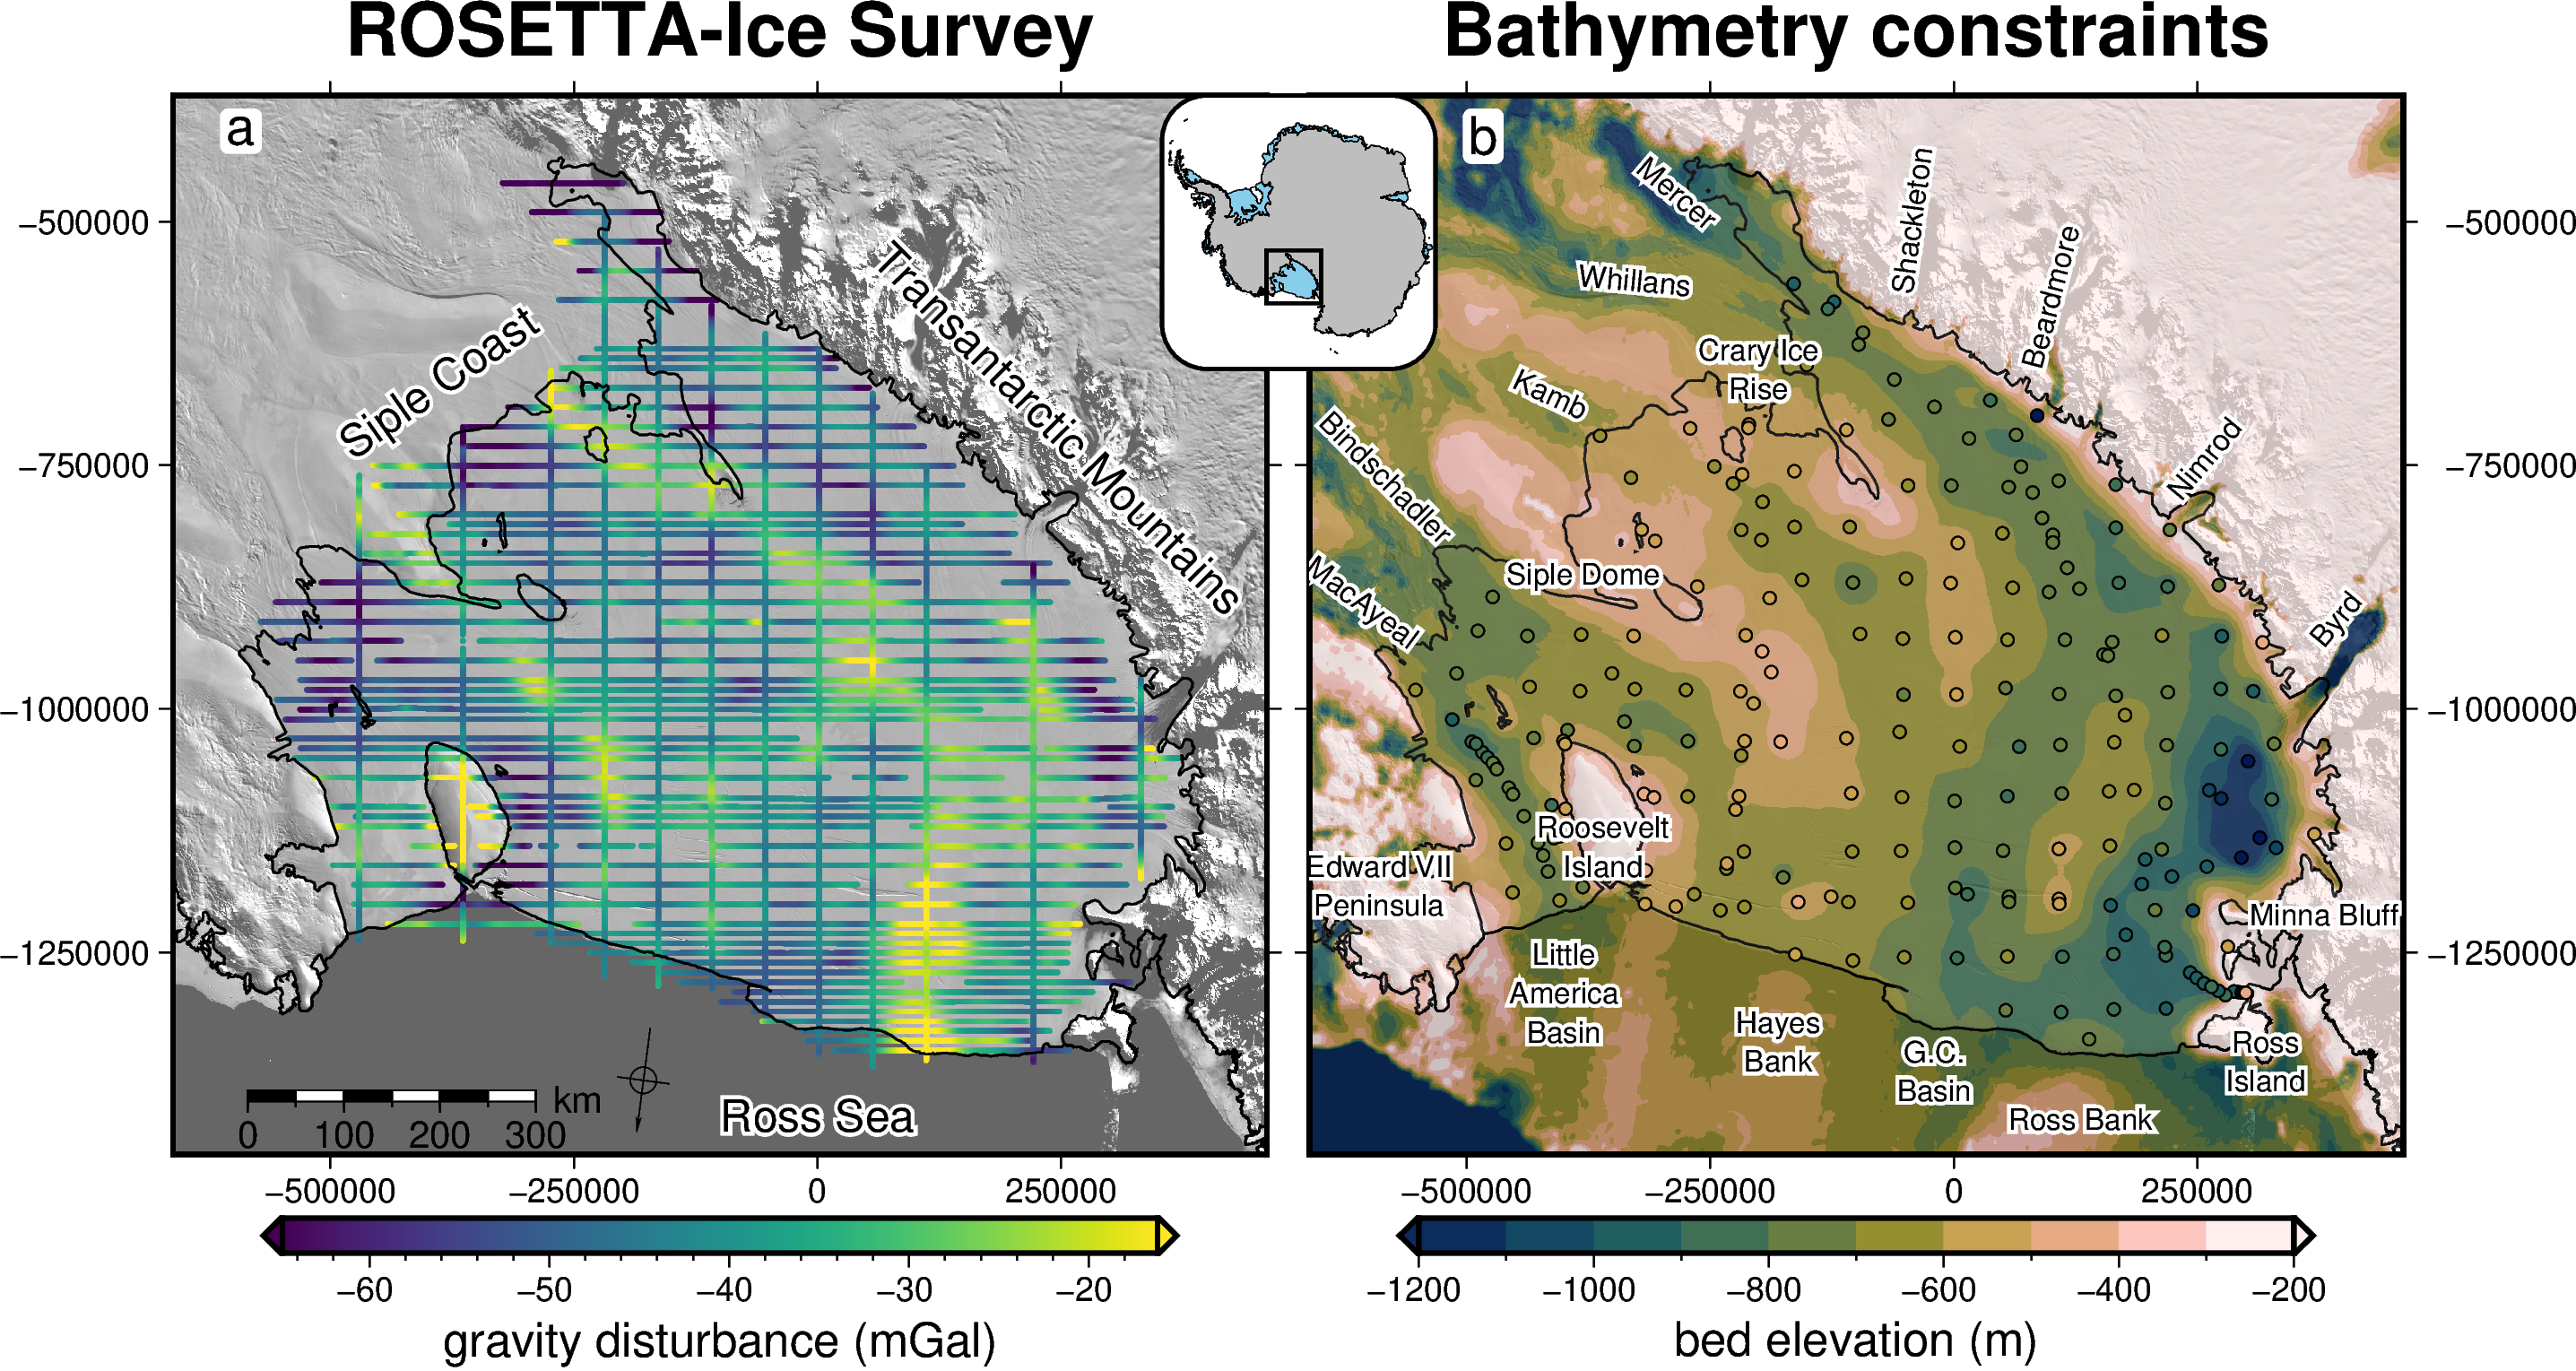
\includegraphics[width=.95\textwidth]{figures/chp4/inversion_inputs.png}
    \caption[Ross Ice Shelf inversion inputs]{Input datasets for the Ross Ice Shelf bathymetry inversion. \textbf{a)} ROSETTA-Ice airborne gravity disturbance data (cleaned and re-levelled). \textbf{b)} Bedmap2 bed elevations in background, with individual constraint points within the ice shelf boundary (dots) on the same colour scale. Black line in both figures shows the grounding line and ice front from \citet{mouginotmeasures2017}. Background imagery is from MODIS-MOA \citep{scambosmodisbased2007}. Regional names shown in \textbf{a} and specific location names shown in \textbf{b}, which include ice streams along the Siple Coast, outlet glaciers along the Transantarctic Mountains, and bathymetry features in the Ross Sea. The RMS difference between the constraint point values and the BedMap2 gridded values is 138~m.}
    \label{fig:chp4_inversion_inputs}
\end{figure}


The largest ice shelf on Earth is the Ross Ice Shelf \citep[Figure \ref{fig:chp4_inversion_inputs},][]{fretwellbedmap22013}. Situated in West Antarctica, along the boundary with East Antarctica, the Ross Ice Shelf comprises ice from both the East and West Antarctic Ice Sheets; a combined catchment totalling 11.6 meters of potential global sea level rise \citep{tintoross2019}. While the Ross Ice Shelf is in approximate steady-state, that is a near net-zero mass change \citep[e.g.,][]{moholdtbasal2014, rignoticeshelf2013}, geologic evidence shows rapid disintegration \citep{naishobliquitypaced2009, yokoyamawidespread2016} and extensive grounding line retreat \citep{venturellimid2020, spectorrapid2017} may have occurred as recently as the mid-Holocene ($\sim7$~kyr B.P.). Ocean forcing, specifically basal melting along the grounding zone, is thought to drive these rapid grounding line retreats \citep{lowrydeglacial2019}. The current stability of the ice shelf is in part attributed to the lack of warm Circumpolar Deep Water penetrating into the cavity \citep{tintoross2019, dinnimanmodel2011}. Ocean waters that do penetrate the cavity, such as High Salinity Shelf Water, are dense and relatively cold. Despite their temperature, they are responsible for significant melting at the large depths of the grounding zone \citep{adusumilliinterannual2020} due to the pressure suppression of the freezing temperature of ice \citep{tintoross2019}. \\

This High Salinity Shelf Water is formed on the continental shelf from the creation of sea ice. Due to their density and the reverse slope of the continental shelf, they flow into the cavity, guided by bathymetric troughs \citep{jacobsmelting1992, tintoross2019}. There are many examples of bathymetric features controlling the routing of these sub-shelf waters \citep[e.g.,][]{dutrieuxstrong2014, derydtgeometric2014, zhaosillinfluenced2019, gladishoceanic2015}. Additionally, ocean modelling sensitivity testing highlights the importance of bathymetric features to sub-shelf circulations and melt \citep{goldbergbathymetric2020, derydtgeometric2014}. Bathymetry, therefore, plays a key role in the stability of the Ross Ice Shelf through its likely control on the basal melt magnitude and distribution \citep{goldberghow2019} and through the buttressing effect of bathymetric pinning points \citep{stillmechanical2019}. \\

Direct observations of the sea floor beneath the Ross Ice Shelf (excluding along its periphery) are limited to two drill holes. The first was the 1977 J9 drill hole north of Crary Ice Rise as part of the Ross Ice Shelf Project \citep{cloughross1979}. The second was the 2017 HWD2 drill hole near the centre of the ice shelf \citep{stevensocean2020}. Apart from these two drill holes, all other inferences of sub-shelf bathymetry depths have been from seismic surveying, or the gravity inversion of \citet{tintoross2019}. The majority of seismic surveys on the Ross Ice Shelf were accomplished during two projects, the International Geophysics Year traverses of the late 1950s and early 1960s \citep{craryglaciological1962,  craryoversnow1959,craryoversnow1962}, and the Ross Ice Shelf Geophysical and Glaciological Survey \citep[RIGGS, 1973-1974][]{bentleyross1984}. These extensive surveys systematically covered the entire ice shelf, collecting 223 observations of bathymetry with a mean spacing of approximately 40 km between points (Figure \ref{fig:chp4_inversion_inputs}b). \\

These seismic and drill hole depths have been included in various Antarctic bed and bathymetry products \citep{fretwellbedmap22013,lebrocqimproved2010, timmermannconsistent2010}. As discussed later, \citet{tintoross2019} conducted a gravity inversion over the entirety of the ice shelf with data from the Ross Ocean and ice Shelf Environment, and Tectonic setting Through Aerogeophysical surveys and modelling project (ROSETTA-Ice). This provided a significantly improved resolution over just the interpolation of the sparse seismic data. This gravity-inverted bathymetry was later incorporated in the BedMachine bed compilation \citep{morlighemdeep2020, morlighemmeasures2022}. This chapter focuses on once again improving the sub-Ross Ice Shelf Bathymetry model. Following \citet{tintoross2019}, we also use a gravity inversion of the ROSETTA-ice data to model the bathymetry. However, we conduct additional processing of the gravity data, and apply an entirely new gravity inversion algorithm, as described in Chapter \ref{ch:3}. Additionally, our method provides an assessment of the spatial uncertainty of the resulting model, a useful component needed for the ocean modelling community \citep{goldbergbathymetric2020}. \\


\section{Methods}

Here we describe the three main methodologies of this chapter; 1) the gravity reduction process (Figure \ref{fig:chp4_workflow}a), 2) the bathymetric inversion process (Figure \ref{fig:chp4_workflow}b), which is explained in detail in Chapter \ref{ch:3} and briefly re-introduced here, and 3) the use of a Monte Carlo simulation to quantify spatial uncertainty in the resulting bathymetry. 

\begin{figure}[!ht]
    \centering
    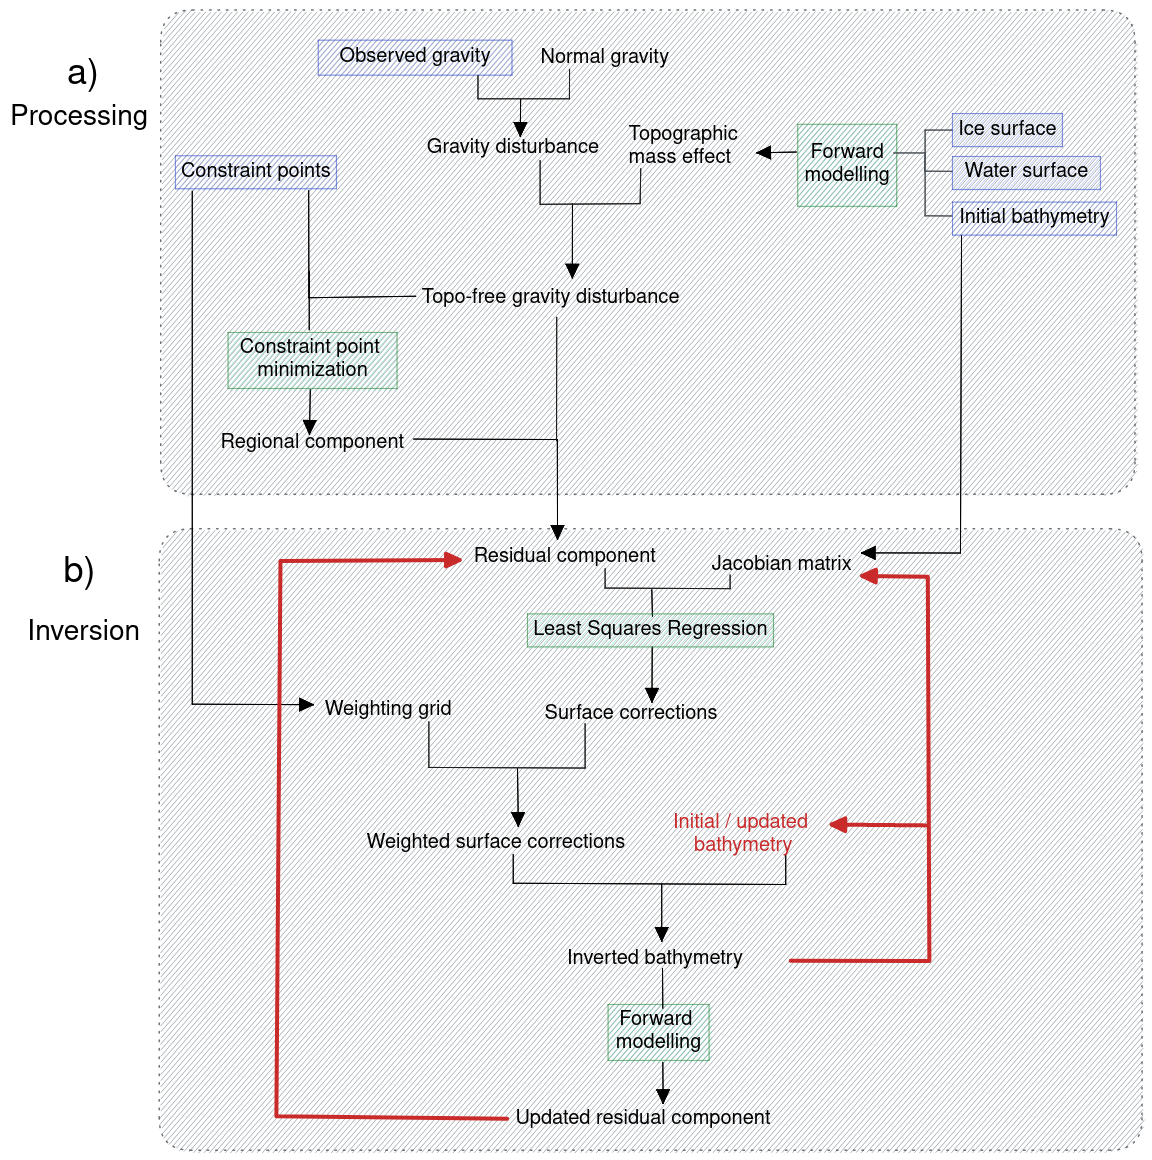
\includegraphics[width=0.95\textwidth]{figures/chp4/Inversion_workflow.png}
    \caption[Schematic inversion workflow diagram]{Schematic workflow diagram for \textbf{a)} gravity processing steps and \textbf{b)} running the inversion. Blue boxes show the input datasets, green boxes show the key processes and red lines signify iterative components of the inversion.}
    \label{fig:chp4_workflow}
\end{figure}

\subsection{Gravity reduction} \label{chp4:gravity_reduction}

A common task in geophysics is the removal of predictable noise to help amplify the signal of interest. This is the basis of gravity reduction; the process of isolating the desired gravity signal from the raw measurements of the Earth's gravitational field. The magnitude of Earth's gravitational acceleration, which we will refer to as \textit{gravity} from here-on, ranges from $\sim$978,000 to $\sim$983,000~mGal, from the equator to the poles, respectively \citep{hofmann-wellenhofphysical2006}. The range in these values, approximately 5000~mGal, vastly outweighs the typical values of gravity anomalies resulting from geologic features of interest. These anomalies of interest are typically on the order of magnitude of 10's of mGal. This exemplifies the issue of removing \textit{noise} which has a significantly greater magnitude than the \textit{signal} of interest. \\

Here, we start the gravity reduction process with observed gravity. We take observed gravity to be the signal which is produced by 1) the gravitational attraction of all massive bodies in Earth and 2) the rotation of the Earth. This means non-geological and time-dependent effects such as machine drift, tidal changes, aircraft manoeuvres and the effect of measuring gravity on a moving platform (E\"{o}tv\"{o}s correction) have already been removed from the observed gravity \citep{hinzenew2005, hinzegravity2013}. With this, observed gravity is defined as;

\begin{equation} \label{chp4:eq:reduction}
    g_{obs}(p) = \gamma(p) + g_{geology}(p)
\end{equation}

\noindent
where, for an observation point $p$, $g_{obs}(p)$ is the observed gravity, $\gamma(p)$ is the attraction of the \textit{normal} Earth and $g_{geology}(p)$ encompasses the gravity effects of all deviations between the \textit{normal} Earth and the real Earth. This \textit{normal} Earth is often taken as a single surface (here the reference ellipsoid) with a constant density above ($\rho_{air}$) and a constant density below ($\rho_{crust}$). Therefore, deviations between the \textit{normal} and real Earth include 1) any masses above the ellipsoid which don't have the uniform density of air or 2) any masses below the ellipsoid which don't have the uniform density of crust. For a bathymetry inversion, the gravity signal of interest is a component of $g_{geology}$, which we must separate from $\gamma$.

\subsubsection{Attraction of normal Earth} \label{ch4 normal gravity}

Observed gravity varies greatly due to the observation point's position, both based on latitude and elevation. Due to the oblate shape of the Earth, gravity is generally lower at low latitudes due to 1) increased distance from the centre of Earth's mass, and 2) more importantly, the increased tangential velocity \citep{jacobygravity2009}. Additionally, there is a decay of gravity with increased elevation, due to an increased distance from the centre of Earth's mass. These effects aren't related to the geologic variations of interest and thus should be removed. Historically, these effects of latitude and elevation were approximated separately, using the International Gravity Formula (\textit{Latitude correction}) and the \textit{Free-air correction}, respectively \citep{hinzenew2005}. Alternatively, \citet{liellipsoid2001} derived an analytical solution to the gravity effects of an ellipsoid, at any point on or above its surface\footnote{Note that the normal gravity calculation with this analytical solution is not valid below the ellipsoid. While this is irrelevant for most locations on Earth, West Antarctic has negative geoid elevations, meaning observations near sea level are likely below the reference ellipsoid, invalidating the normal gravity calculation. For these situations, the use of a quasi-ellipsoid is recommended \citep{vajdagravity2008, paštekaunderstanding2017}}. With this, the Latitude and Free-air corrections are combined, and their approximations are replaced with closed-form solutions. By subtracting the normal gravity from the observed gravity at each observation point the gravity disturbance is found, where

\begin{equation} \label{disturbance}
    \delta g(p) = g_{obs}(p) - \gamma(p),
\end{equation}

\noindent
where for an observation point $p$, $\delta g(p)$ is the gravity disturbance, $g_{obs}(p)$ is the observed gravity, and $\gamma(p)$ is the normal gravity \citep{paštekaunderstanding2017}. \\

The observation point, $p$, is defined by three coordinates; latitude, longitude, and geometric height (ellipsoidal height). It is a common mistake in geophysical studies for the normal gravity calculation to use the point $p$'s orthometric height (geoidal height or mean sea level), instead of its geometric height \citep{oliveirashould2018}. This results in the calculation of normal gravity at a different point in 3D space relative to the observation. This calculation, while truly determining the gravity anomaly (a.k.a. free-air anomaly), is not well-suited for geological interests because the gravity anomaly contains signal from centrifugal acceleration effects due to the different locations of the points. Conversely, the gravity disturbance is defined as the difference between gravity and normal gravity at the same point, and thus only contains signal resulting from geologic sources \citep{hofmann-wellenhofphysical2006}. The difference between the gravity anomaly and the disturbance for Antarctica ranges from -20 to +20~mGal (See Figure \ref{fig:appC_disturbance_vs_anomaly} in appendix \ref{appendix:C} for a comparison). It is common for studies to correctly use the gravity disturbance while referring to it as the free-air anomaly to adhere to tradition. Combining Equations \ref{chp4:eq:reduction} and \ref{disturbance}, shows that the gravity disturbance, $\delta g$, results solely from deviations between the theoretical model of the Earth (the \textit{normal} Earth) and the true density variations and topography of the Earth \citep{vajdaremoval2004}. Figure \ref{fig:chp4_antarctic_gravity_reduction} compares the observed gravity, the normal gravity, the gravity disturbance, and the gravity anomaly for Antarctica. \\

\begin{figure}[!ht]
% \renewcommand\thesubfigure{\arabic{subfigure}}
  \centering
    \begin{subfigure}[t]{.9\textwidth}
        \centering
        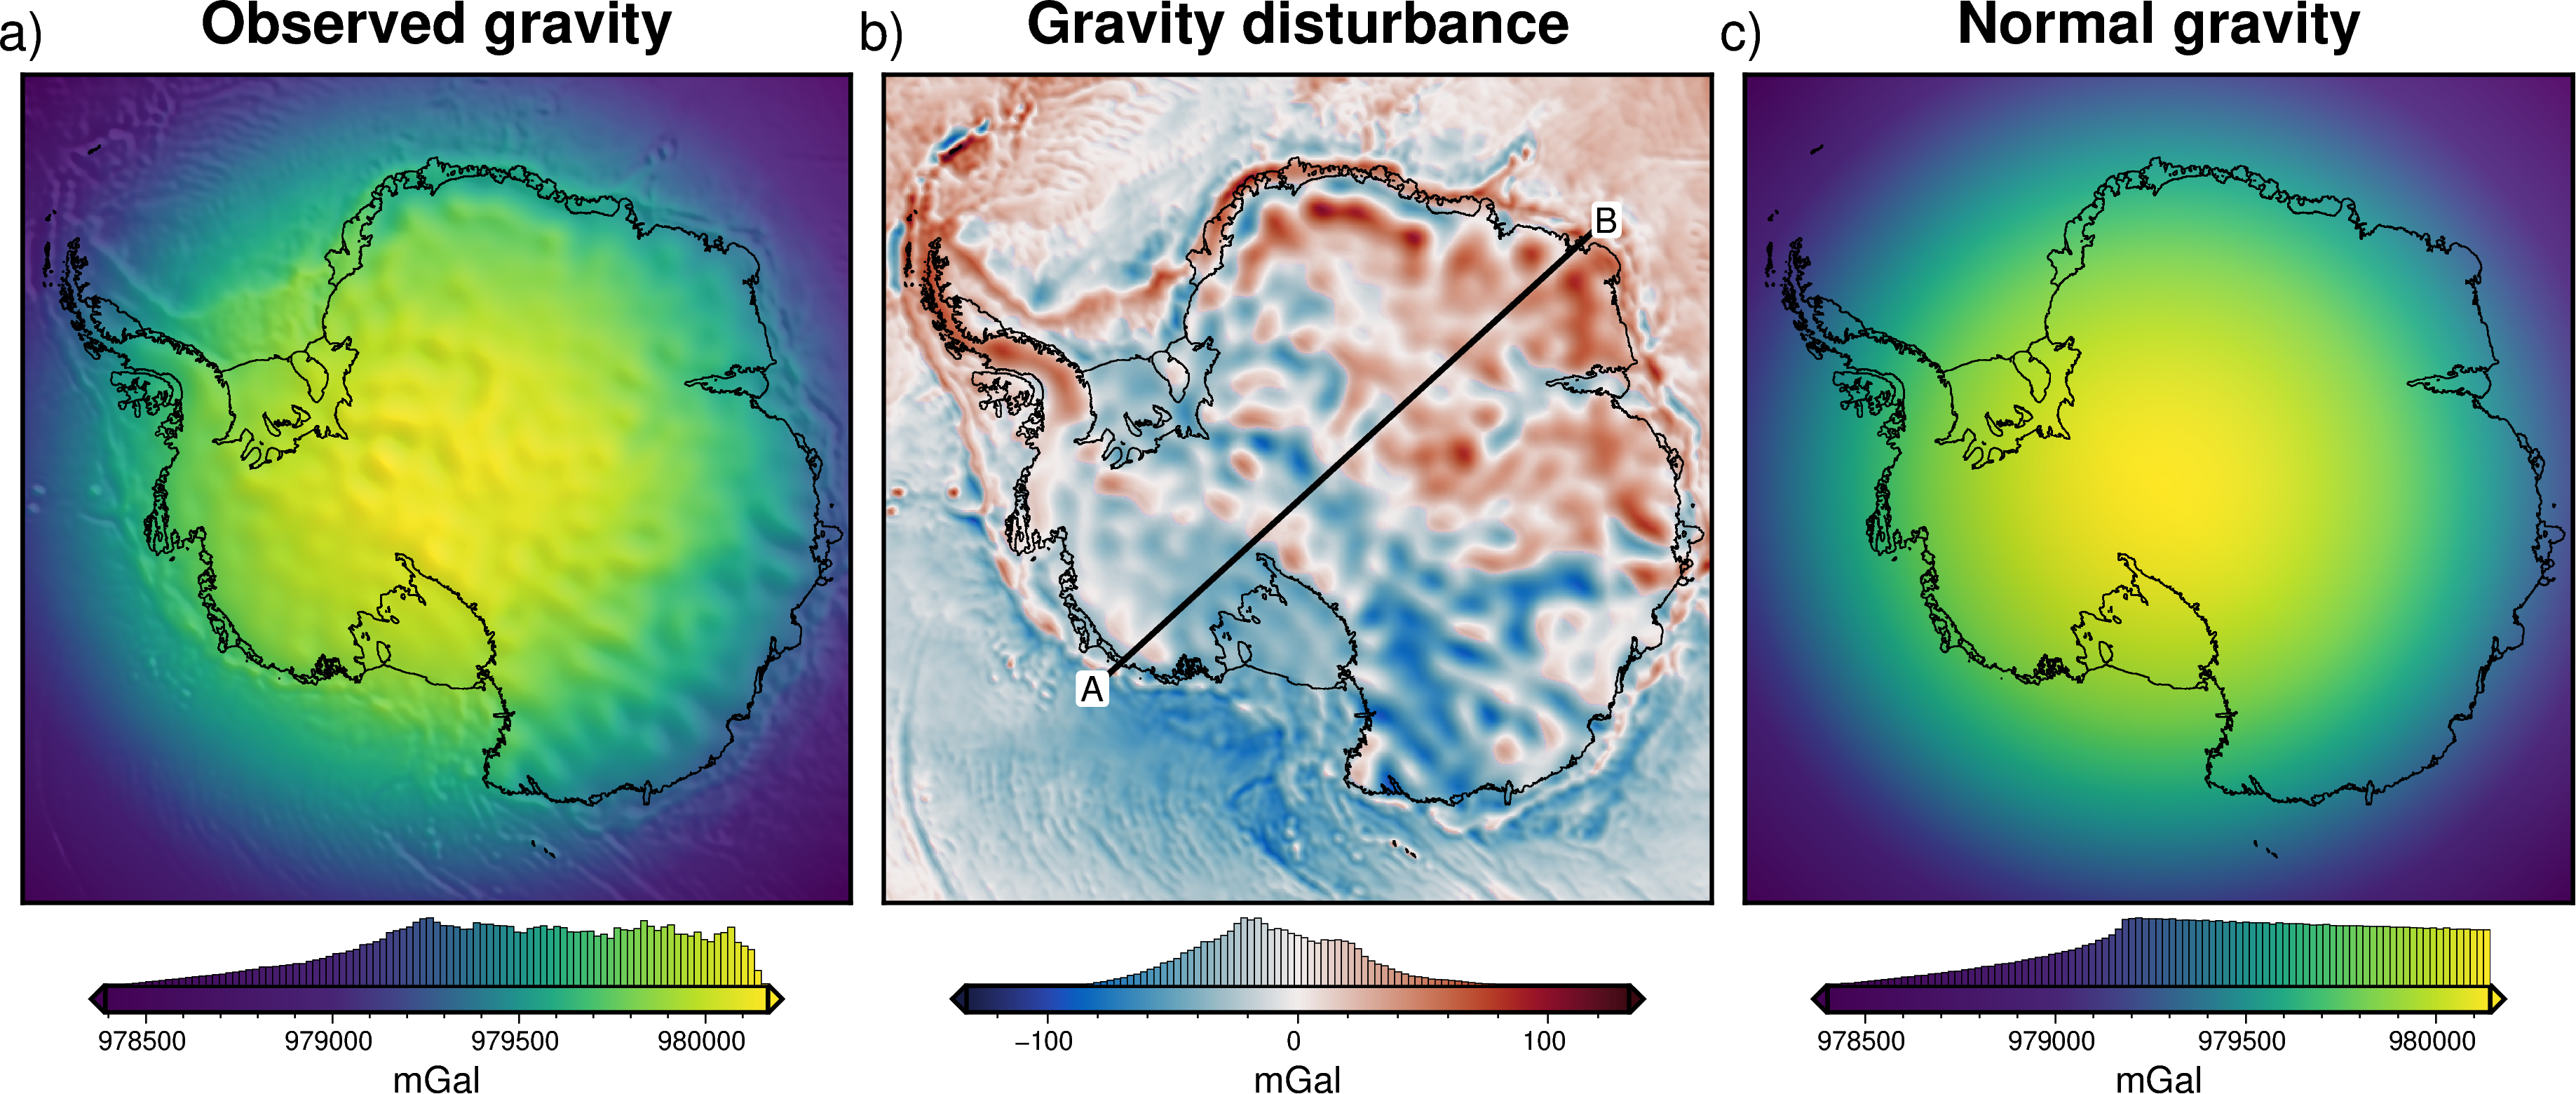
\includegraphics[width=\textwidth]{figures/chp4/antarctic_gravity_disturbance_with_profile}
        % \caption{}
    \end{subfigure}
    \begin{subfigure}[t]{.7\textwidth}
        \addtocounter{subfigure}{3}
        \centering
        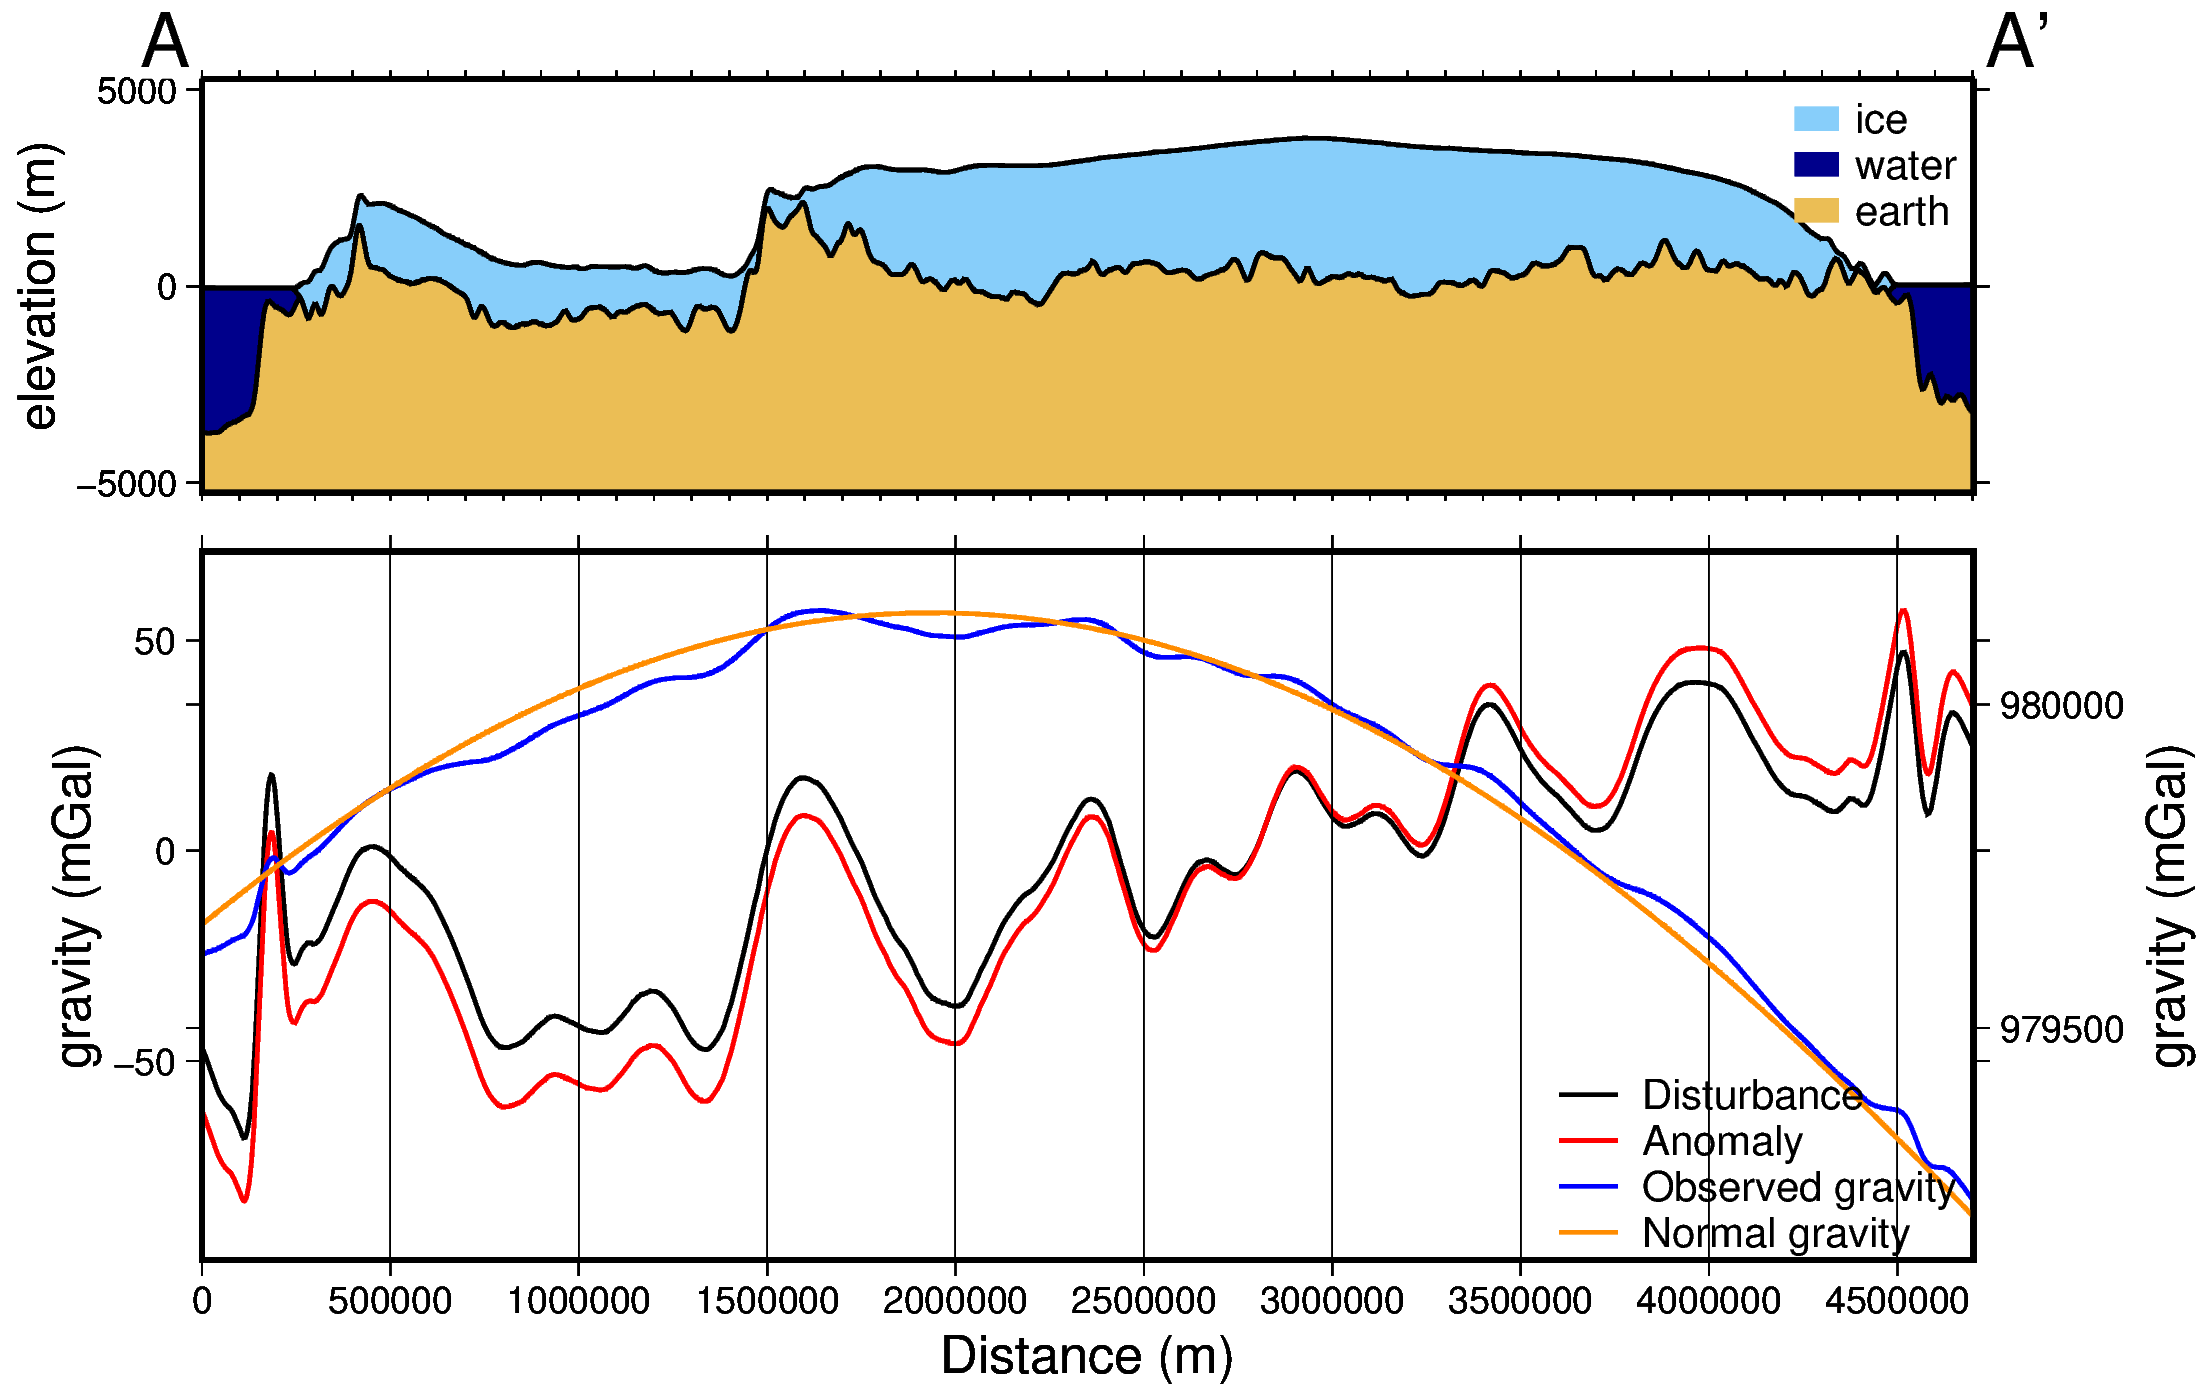
\includegraphics[width=\textwidth]{figures/chp4/antarctic_gravity_profile}
        \caption{}
    \end{subfigure}
  \caption[Observed gravity data reduction for Antarctica]{Observed gravity data reduction for Antarctica. \textbf{a)} Observed gravity data from \citet{försteeigen6c42014} at a geodetic observation height of 10~km. \textbf{b)} The gravity disturbance at 10~km height, defined as \textbf{a}-\textbf{c}. \textbf{c)} The normal gravity calculated at the same observation points as \textbf{a} using the closed-form equations of \citet{liellipsoid2001}. \textbf{d)} Profile A-B across Antarctica, location shown in \textbf{b}. Gravity disturbance (black) and anomaly (red) values are on the left y-axis, while observed (blue) and normal (orange) gravity values are on the right y-axis.}
    \label{fig:chp4_antarctic_gravity_reduction}
\end{figure}

\subsubsection{Topographic mass effects} \label{chp4_topo_mass_effect}

Typically, geophysical studies are interested in interpreting or inverting gravity signals resulting from subsurface features. To accommodate this, all other gravity effects must be computed and removed from the gravity disturbance. These other effects include the gravity resulting from masses bound by known surfaces, referred to as \textit{topographic} or \textit{terrain masses}. These surfaces include, but are not limited to, the rock surface (topography), the ocean surface (geoid), the seafloor (bathymetry), and the ice surface. Together, the gravity resulting from these masses is referred to as the \textit{topographic mass effect}. Correcting the gravity disturbance for these topographic masses yields the \textit{topo-free gravity disturbance} $\delta g_{TC}$, where

\begin{equation} \label{chp4:eq:bouguer_disturbance}
    \delta g_{TC}(p) = \delta g(p) - g_{topo}(p).
\end{equation}

$g_{topo}(p)$ represents the summed topographic mass effect. $\delta g_{TC}$ is sometimes referred to as the \textit{Bouguer disturbance}, owing to the historic use of the \textit{Bouguer anomaly}. In accordance with \citet{vajdasecondary2007}, we refer to it as the \textit{topo-free gravity disturbance} to clarify that the ellipsoid has been used instead of the geoid in all reduction steps. In the past, the topographic mass effect has been split into the Bouguer slab correction and the terrain correction. The Bouguer slab correction approximates the topographic masses as laterally infinite flat slabs, while the terrain correction accounts for the overestimation of the Bouguer slab resulting from the assumption of the flat slab. With modern computing able to efficiently calculate the gravity resulting directly from a topographic surface \citep{fatiandoaterraprojectharmonica2023}, there is no need for the separate two-step correction. \\

\begin{figure}[!ht]
    \centering
    \includesvg[inkscapelatex=false,width=0.98\textwidth]{chp4/terrain_effects}
    \caption[Components of the topographic mass effect]{Components of the topographic mass effect and resulting topo-free gravity disturbance, or Bouguer disturbance. \textbf{a)} The normal Earth model, \textbf{b)} a simplified real Earth model. \textbf{c)} Topographic masses separated into components above and below the ellipsoid. \textbf{d)} Real Earth topographic masses which are anomalous with respect to the normal Earth. Note if the reference level (red dashed line) is switched from the ellipsoid to the geoid, this would result in a Bouguer \textit{anomaly}.}
    \label{fig:chp4_terrain_effects}
\end{figure}

The topographic mass effect reflects all topographic deviations (including topography of the ice, water, and seafloor) between the \textit{normal} Earth and the real Earth. The \textit{normal} Earth model is shown in Figure \ref{fig:chp4_terrain_effects}a, as defined by air above the ellipsoid and crust below. A simplified model of the true Earth is shown in Figure \ref{fig:chp4_terrain_effects}b, and contains air, ice, water, crust, and various geologic bodies within the crust. These masses are separated in Figure \ref{fig:chp4_terrain_effects}c into components above and below the ellipsoid. From this, the masses which are anomalous with respect to the \textit{normal} Earth can be distinguished, as shown in Figure \ref{fig:chp4_terrain_effects}d. These anomalous masses include water, ice, and crust above the ellipsoid, and air, ice, water, and geologic bodies below the ellipsoid. The gravitational effect of these anomalous masses can be approximated by assuming each mass's density and setting it relative to the density of the component of the \textit{normal} Earth which the mass is replacing. These relative densities are shown in the key of Figure \ref{fig:chp4_terrain_effects}d. Calculating and summing the gravity effect of each of the components of Figure \ref{fig:chp4_terrain_effects}d (excluding the geologic bodies) gives the topographic mass effect. Subtracting this from the gravity disturbance gives the topo-free gravity disturbance\footnote{The use of the reference ellipsoid as the bounding surface of the topographic mass effect calculations results in a topo-free gravity disturbance while using the geoid as the bounding surface would result in a Bouguer anomaly \citep{vajdanew2006}.}.\\

\begin{figure}[!ht]
    \centering
    \includesvg[inkscapelatex=false,width=0.98\textwidth]{chp4/discretizing_terrain_mass_effect}
    \caption[Discretizing the topographic mass effect]{Discretizing the topographic mass effect. \textbf{a)} The simplified real Earth model, with air, ice, water, and earth. \textbf{b)} the resulting anomalous masses relative to the \textit{normal} Earth, as shown in Figure \ref{fig:chp4_terrain_effects}d. \textbf{c)} Prisms between the ellipsoid and the ice surface, \textbf{d)} prisms between the ellipsoid and the water surface (ice base), and \textbf{e)} prisms between the ellipsoid and the rock surface (topography onshore and bathymetry offshore). Overlap of prisms from \textbf{c-e} creates the different shades shown in \textbf{b}. The alternative discretization approach, commonly used, is shown in \textbf{f-h} where the prism layers are bound both above and below by topographic layers, or arbitrary references (bottom of prisms in \textbf{h}), instead of by the normal Earth reference surface (ellipsoid). Additionally, density values of the prisms are related to the material they discretize and are not relative to the expected density of the normal Earth.}
    \label{fig:chp4_discretized_topo_mass_effect}
\end{figure}

To compute the topographic mass effect, the anomalous masses from Figure \ref{fig:chp4_terrain_effects}d are discretized into a series of vertical right-rectangular prisms. To achieve the geometry and density configuration of Figure \ref{fig:chp4_terrain_effects}d, three sets of prisms are used, as shown in Figure \ref{fig:chp4_discretized_topo_mass_effect}c-e. 

\begin{enumerate}
    \item Prisms between the ice surface and the ellipsoid are assigned densities of $\rho_{ice} - \rho_{air}$ for prisms above the ellipsoid, and $\rho_{air} - \rho_{ice}$ for prisms below the ellipsoid. 
    \item Prisms between the water surface (ice base) and the ellipsoid are assigned densities of $\rho_{water} - \rho_{ice}$ for prisms above the ellipsoid, and $\rho_{ice} - \rho_{water}$ for prisms below the ellipsoid. 
    \item Prisms between the rock surface (topography onshore and bathymetry offshore) and the ellipsoid are assigned densities of $\rho_{earth} - \rho_{water}$ for prisms above the ellipsoid, and $\rho_{water} - \rho_{earth}$ for prisms below the ellipsoid. 
\end{enumerate}

This configuration of prisms correctly discretizes the topographic mass effect because the ice surface is equal to the water surface in areas of no ice thickness, and the water surface is equal to the rock surface in areas of no water thickness. Due to this, the overlap between the three sets of prisms, shown in Figure \ref{fig:chp4_discretized_topo_mass_effect}b gives the appropriate densities, as defined in Figure \ref{fig:chp4_terrain_effects}d. From these three sets of prisms, the topographic mass effect can be calculated at the gravity observation points using the analytical solutions of \citet{nagygravitational2000}. As a demonstration, the topographic mass effect for Antarctica is calculated using topographic data from Bedmap2 \citep{fretwellbedmap22013}, referenced to the WGS-84 ellipsoid. The observed satellite gravity data has a low spatial resolution, so the lower resolution of Bedmap2 over BedMachine v3 is insignificant. The calculated topographic mass effect, the gravity disturbance, the resulting topo-free gravity disturbance, and the topographic mass effect from the alternative method of discretization (Figure \ref{fig:chp4_discretized_topo_mass_effect}f-h) are shown in Figure \ref{fig:chp4_antarctic_topo_free_disturbance}.\\

\begin{figure}[!ht]
% \renewcommand\thesubfigure{\arabic{subfigure}}
  \centering
    \begin{subfigure}[t]{.9\textwidth}
        \centering
        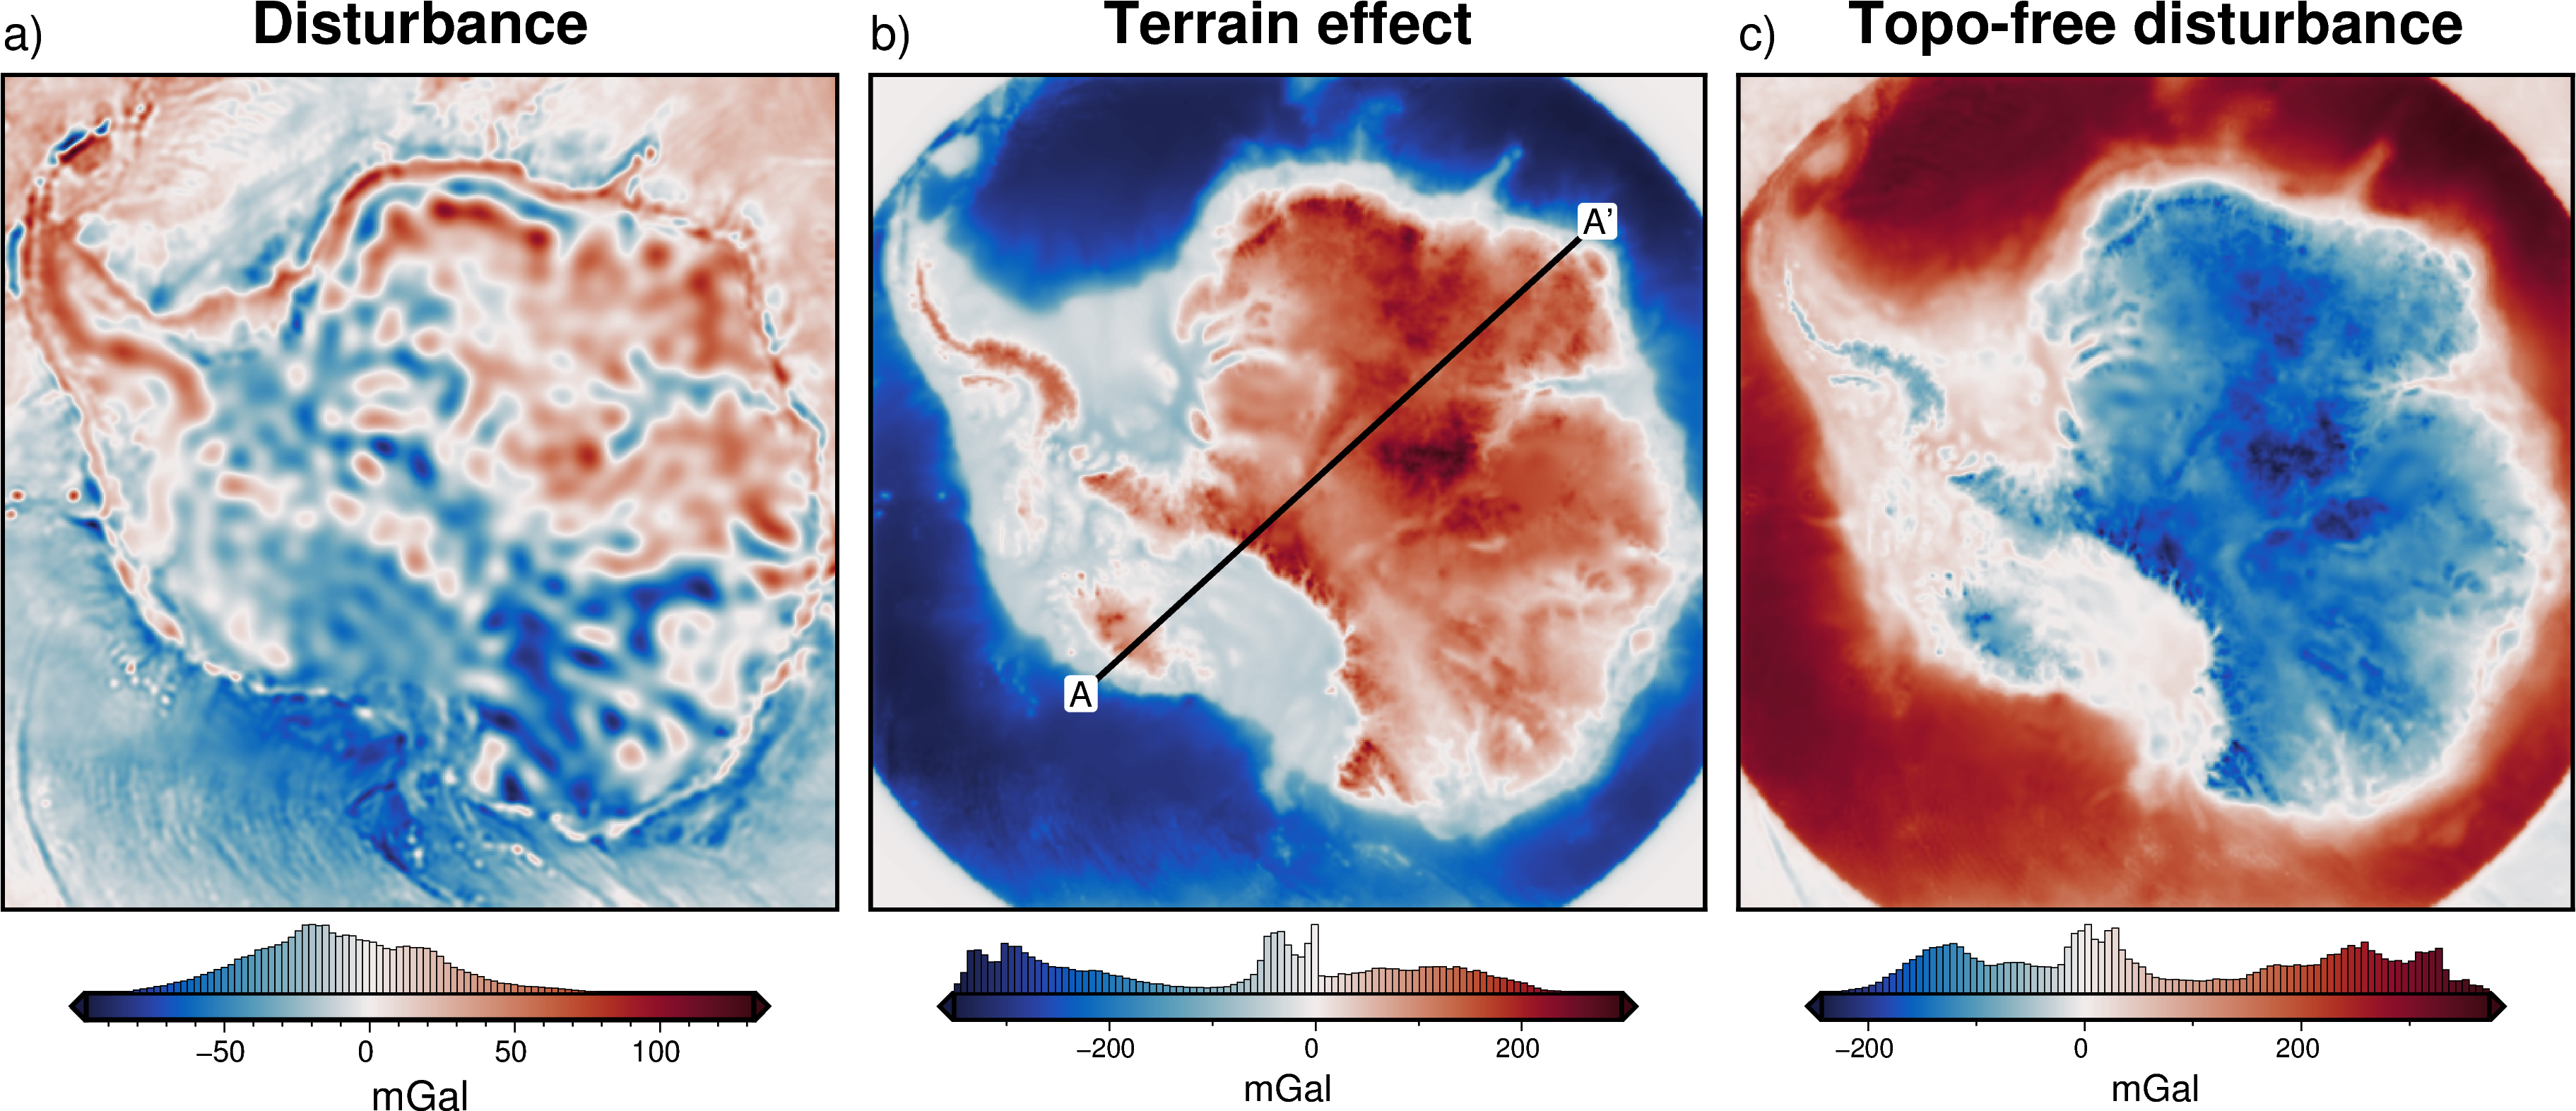
\includegraphics[width=\textwidth]{figures/chp4/antarctic_topo_free_disturbance.png}
        % \caption{}
    \end{subfigure}
    \begin{subfigure}[t]{.7\textwidth}
        \addtocounter{subfigure}{3}
        \centering
        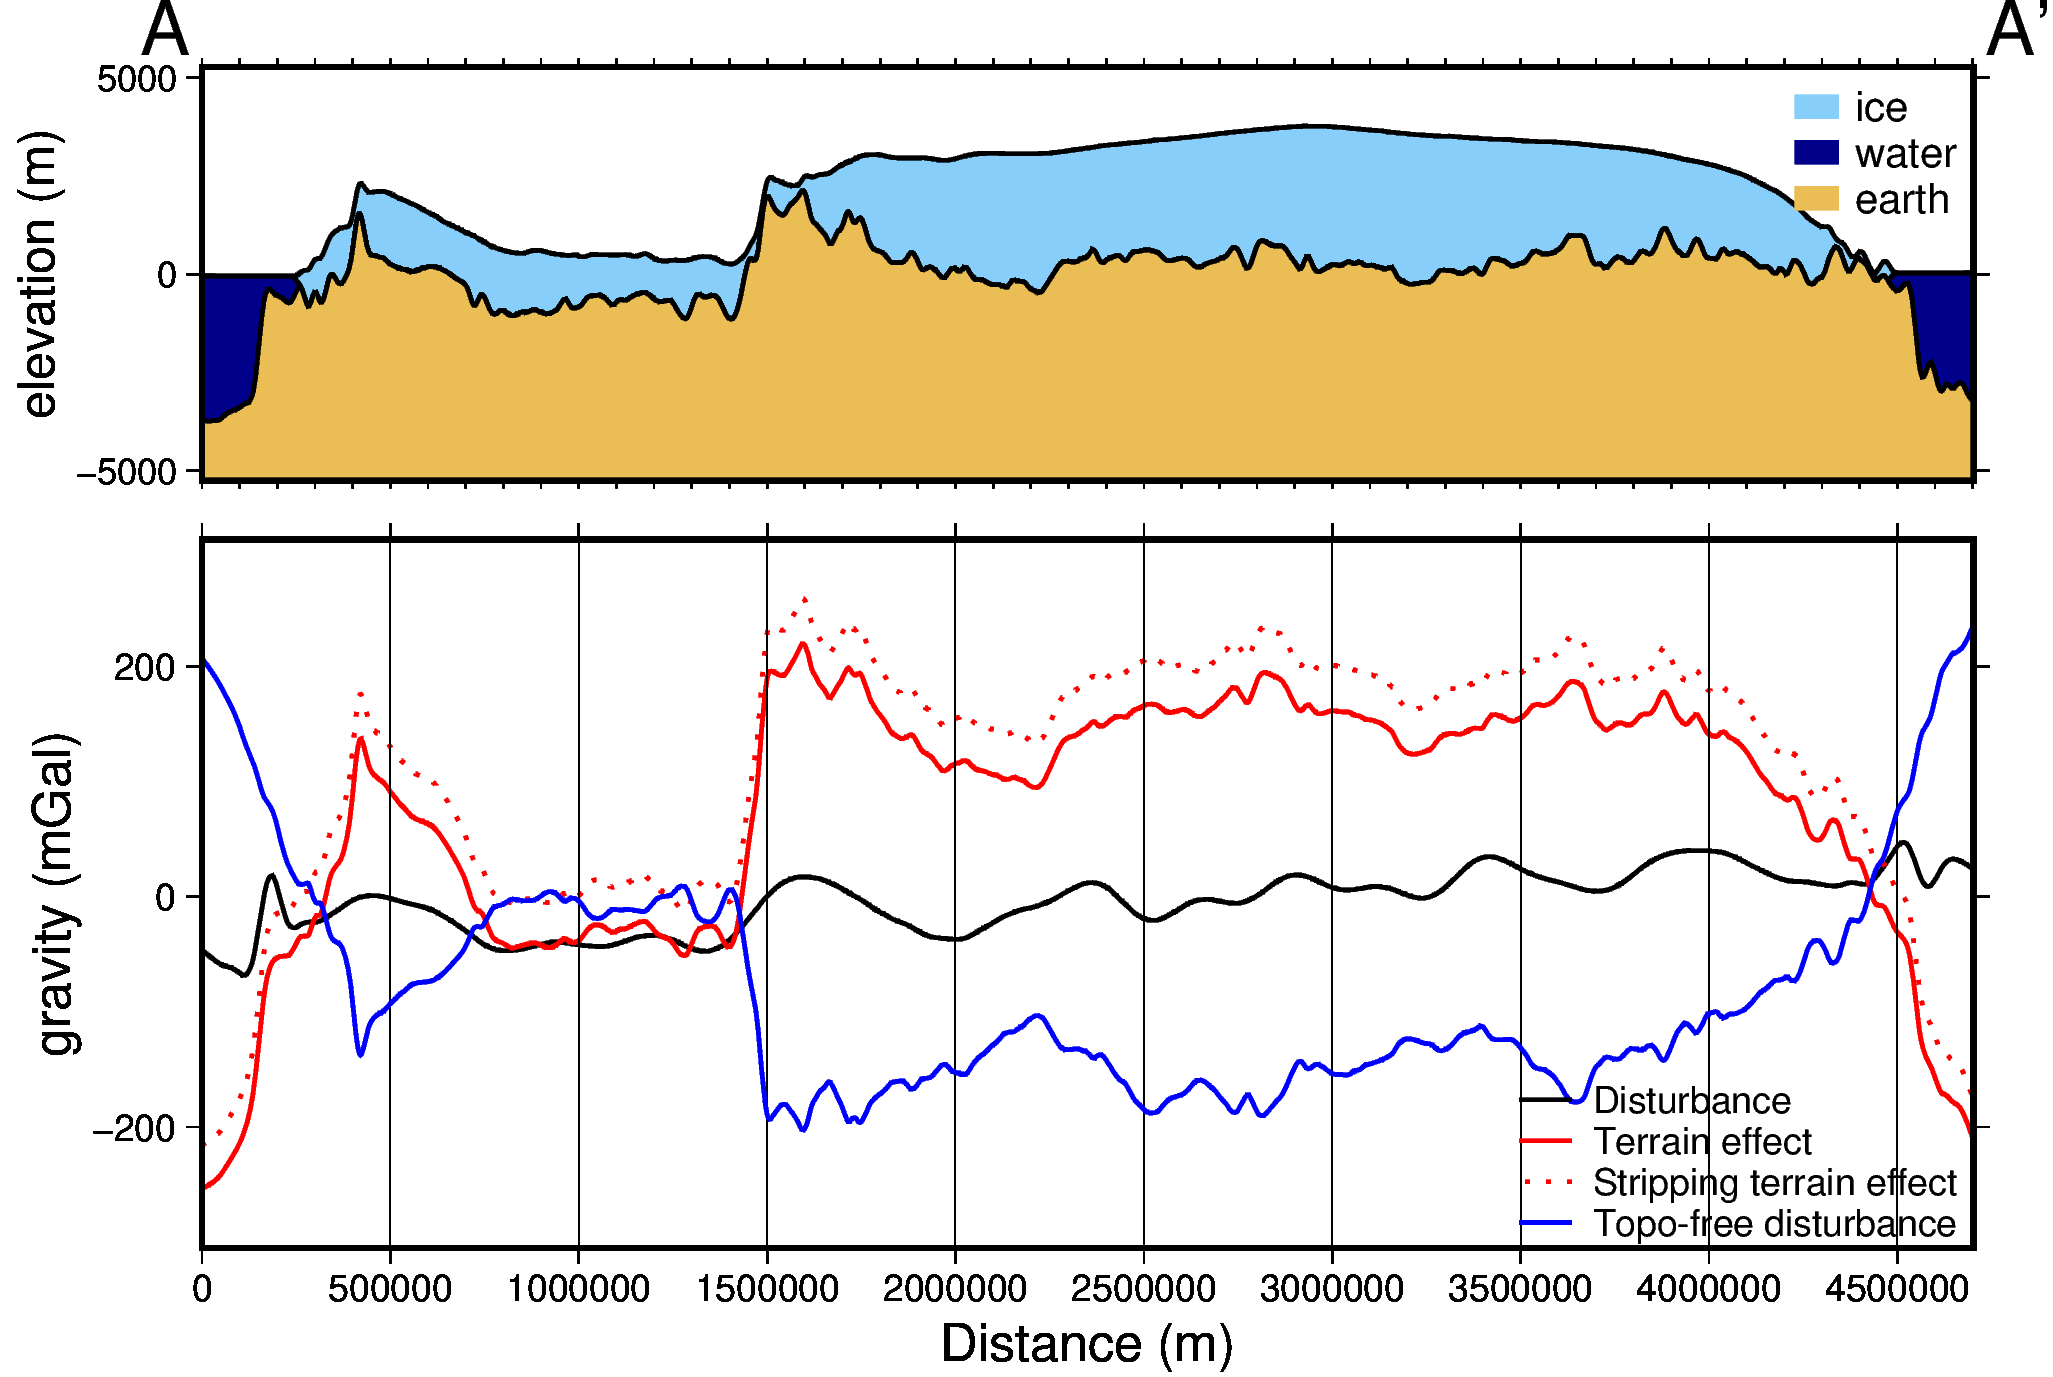
\includegraphics[width=\textwidth]{figures/chp4/antarctic_topo_free_disturbance_profile.png}
        \caption{}
    \end{subfigure}
  \caption[Topographic mass effect for Antarctica]{Topographic mass effect at 10~km height for Antarctica, from Bedmap2 topographic data \citep{fretwellbedmap22013}. \textbf{a)} Gravity disturbance at a geodetic observation height of 10~km, from Figure \ref{fig:chp4_antarctic_gravity_reduction}b. \textbf{b)} The combined gravity effect of the anomalous masses defined in Figure \ref{fig:chp4_terrain_effects}d and discretized following \ref{fig:chp4_discretized_topo_mass_effect}b. \textbf{c)} The topo-free gravity disturbance, calculated as \textbf{a} - \textbf{b}. \textbf{d)} Profile A-A' across Antarctica, location shown in \textbf{b}. The dotted red line shows the terrain mass effect results of the alternative discretization method shown in Figure \ref{fig:chp4_discretized_topo_mass_effect}f-h. A DC shift was applied to attempt to remove the offset.}
    \label{fig:chp4_antarctic_topo_free_disturbance}
\end{figure}

The theoretical topo-free gravity disturbance is the gravity effect caused by and only by anomalous subsurface bodies, which have a density different from the assumed constant density of the crust. In reality, there are additional components of the topo-free gravity disturbance resulting from 1) noise in the observed data, 2) non-uniform densities used in the topographic mass effect calculation, and 3) inaccurate topographic data used for the topographic mass effect calculation. In most geophysical applications, the uncertainty of the topographic data is small compared to other uncertainties in the analysis, and thus component \#3 is assumed to be zero. Conversely, for the case of a bathymetry inversion, this component of the topo-free disturbance resulting from the inaccuracies of the topography (bathymetry) data is the signal of interest. Next, we will isolate this component from the remainder of the topo-free gravity disturbance.\\

\subsubsection{Regional separation} \label{chp4_regional_separation_method}

Here, we separate the topo-free gravity disturbance into components resulting from 1) subsurface geologic variations and 2) inaccuracies between the true bathymetry and the low-resolution bathymetry data used for the terrain mass effect. These are referred to as the regional and residual components, respectively. Chapter \ref{ch:3} highlighted the importance of accurately estimating and separating this regional component from the residual. The regional estimation was found to be the largest source of uncertainty in several synthetic bathymetry inversions, as well as other Antarctic bathymetry inversions \citep{brisbourneseabed2014}. While there are many techniques to estimate the regional component, we will use constraint point minimization due to its demonstrated effectiveness over the other methods (Section \ref{chp3_regional_seperation}). This technique samples the topo-free gravity disturbance at points of known bathymetry depth, referred to as the constraint points. Since the depth is known here, the residual component of gravity should be near zero, and thus the regional component should entirely equal the topo-free gravity disturbance. Using these sampled values, the entire model domain is gridded with an interpolation, using either bi-harmonic splines \citep{uiedaverde2018} or minimum curvature \citep{smithgridding1990}. The resulting grid makes up the regional component, and when subtracted from the topo-free gravity disturbance gives the residual component. This residual component is the input into the inversion.\\ 

\subsection{Bathymetry inversion} \label{ch4_inversion_method}

Here we start by briefly summarising the bathymetry inversion workflow described in Chapter \ref{ch:3}, and shown schematically in Figure \ref{fig:chp4_workflow}b. Then we compare our method to several other commonly used bathymetry inversion algorithms. The basis of modelling bathymetry with a gravity inversion is that the bathymetry surface, which is a contrast between lower-density material (seawater) and higher-density material (sediment) creates a measurable effect on Earth's gravity. Our inversion begins by computing the Jacobian matrix (Equation \ref{eq:jacobian}), which is a quantitative means of describing the sensitivity of the residual gravity data to changes in the height of each grid cell of bathymetry. In other words, the Jacobian quantifies the ratio between the amplitude of bathymetric features and the gravity anomaly resulting from them. From this Jacobian matrix, the optimal change to apply to each bathymetry grid cell to minimize the residual gravity data is estimated. This is in the form of a surface correction grid, with a value for each grid cell of bathymetry. Since there are locations of already known bathymetry depths (constraint points), this surface correction grid should be zero at these points. To achieve this, a weighting grid is calculated (Section \ref{chp3:regularization}), which is based on the minimum distance between each grid cell and the nearest constraint point. These distance values are then normalized from 0 to 1, with 0 being the cells closest to the constraints, and 1 being the cells furthest. The surface correction grid is multiplied by this weighting grid, to achieve a correction value of 0 m at the constraints, smoothly tapering off to the full estimated correction values at a distance.\\

With this weighted surface correction grid, the original bathymetry depths are updated. To ensure the updated bathymetry doesn't intersect the ice base, the ice base topography is set as an upper-bounding surface. The forward gravity of this updated bathymetry is then re-calculated, with the prism configuration and densities shown in Figure \ref{fig:chp4_discretized_topo_mass_effect}e. The updated forward gravity is used to recalculate the topo-free gravity disturbance. Using the same regional component as calculated before the inversion (Section \ref{chp4_regional_separation_method}), an updated residual gravity is computed. This is then input into the next iteration of the inversion (red lines in Figure \ref{fig:chp4_workflow}b). Iterations continue until a set of user-defined stopping criteria are met; 1) a maximum number of iterations is reached, 2) a minimum value of the $\ell^2$-norm of the residual is reached, or 3) there is no significant variation in the $\ell^2$-norm in two consecutive iterations.\\

This process describes a single \textit{inversion}. The critical step in this inversion, determining the surface correction values from the sensitivity matrix, includes a damping parameter that controls the smoothness of the resulting inverted bathymetry. This damping parameter value directly affects the resulting bathymetry model and needs to be carefully chosen. For this, we follow the cross-validation routine described in Chapter \ref{ch:3} from \citet{uiedafast2017}. This involves running the entire inversion for a suite of different damping parameter values. The input gravity data to these inversions is split into a \textit{testing} set and a \textit{training} set. The inversion only uses the \textit{training} set. After each inversion, the forward gravity effect of the updated bathymetry model is calculated at the points of the \textit{testing} set. The root mean squared difference between the testing gravity values and the forward gravity values gives the \textit{score} of each cross-validation. The damping parameter which produces the lowest score is chosen as the optimal value.\\


\subsection{Starting bathymetry} \label{chp4_starting_bed_method}

An initial bathymetry model for the inversion is needed to compute the topographic mass effect and to run the inversion. The weighting grid constrains the inversion from changing the starting grid values at the constraint points. For this reason, the starting model should be carefully created. As discussed in the previous chapter (Chapter \ref{ch:3}, Section \ref{chp3_gridding_comparison}), there are several methods of creating the starting model from the sparse measurements at the constraint points. Here, we use and compare two techniques for interpolating these constraint point values over the entire domain; tensioned minimum curvature \citep{smithgridding1990} and bi-harmonic splines \citep{sandwellbiharmonic1987}. See Chapter \ref{ch:3} Section \ref{chp3_gridding_comparison} for the details of these gridding techniques.\\

\subsection{Uncertainty quantification} \label{chp4_uncertainty_method}

A major component missing from many bathymetry inversions is assessing the spatially variable uncertainty in the resulting bathymetry depths. This uncertainty arises from a multitude of sources, including uncertainty in 1) the gravity data measurements, 2) constraint point depths, 3) user-defined variables, such as ice, water, or sediment density, and 4) uncertainties associated with the various methodologies of the inversion. Here we use a sampling-based approach to estimate the uncertainty, where the uncertainty of the \textit{inputs} is used to assess the uncertainty of the \textit{output}, in this case, the inverted bathymetry. This general method of uncertainty analysis is referred to as Monte Carlo sampling \citep{jansenmonte1994}.\\

For a generalized problem of inputs $\textbf{x}$ and a function $\textbf{y(x)}$, Monte Carlo simulation provides a means to answer the two following questions; 1) what is the uncertainty in $\textbf{y(x)}$ given the uncertainty in $\textbf{x}$? and 2) what are the relative importance of the various components of $\textbf{x}$ with respect to $\textbf{y(x)}$ \citep{heltonsurvey2006}? While there are many components that contribute to the overall inversion uncertainty, here we will examine 1) uncertainty in the gravity data values, 2) depth uncertainty of the constraint points, 3) uncertainty in the chosen density values used for ice, water, and earth, and 4) uncertainties related to user-chosen parameter values in the inversion. Uncertainties that are not covered here are those which relate to processes of the inversion which don't have associated measurable input uncertainties. This includes the use of spatially non-variable density values for ice, water, or earth, or the effects of discretizing a real topographic surface as a series of prisms.\\

The Monte Carlo simulation consists of sampling the input parameters $N$ times from their respective distributions (Figure \ref{fig:chp4_Monte_Carlo_workflow}b) and running the entire inversion workflow for each of the $N$ parameter sets (Figure \ref{fig:chp4_Monte_Carlo_workflow}c). For each bathymetry grid cell, the weighted standard deviation of the $N$ resulting inverted bathymetries is found (Figure \ref{fig:chp4_Monte_Carlo_workflow}d). This grid of cell-specific standard deviations show where the input parameters have a large effect on the bathymetry results. This grid is used as our estimate of the spatial uncertainty in the inversion. The grid of cell-specific weighted median values is then taken to be the optimal inversion result. These cell-specific statistics are weighted by the inverse square of each inverted bathymetry's RMS difference with the constraint point depths (Figure \ref{fig:chp4_Monte_Carlo_workflow}d). This reduces the bias of inversions in the ensemble which performed poorly, as defined by not adhering to the constraints \citep{schnaidtbootstrap2015}. To assess the relative importance of the input parameters, in addition to the complete Monte Carlo simulation, additional simulations are run where each parameter's effect is isolated. For these, only a singular parameter is sampled from its distribution, so that the resulting spatial standard deviation is due solely to the uncertainty of that parameter.\\

\begin{figure}[!ht]
    \centering
    \includegraphics[width=0.99\textwidth]{figures/chp4/Monte_Carlo_workflow.png}
    \caption[Schematic Monte Carlo workflow diagram]{Schematic workflow diagram for the Monte Carlo uncertainty analysis. \textbf{a)} The Monte Carlo simulation, consisting of \textbf{b)} sampling the inputs from their respective distributions, and \textbf{c)} implementing the various components of the workflow, depending on which inputs have been sampled. This process is repeated $N$ times, yielding $N$ inverted bathymetry grids. \textbf{d)} Weighted cell-specific statistics are computed. Each inverted bathymetry grid (large purple boxes) is weighted by the respective inversion's constraint depth RMSE. These weights are used to compute the weighted mean and weighted standard deviation of each grid cell (bold purple square).}
    \label{fig:chp4_Monte_Carlo_workflow}
\end{figure}

The parameters included in the Monte Carlo sampling are: 1) the gravity disturbance data, 2) the constraints point depths, 3) the gridding parameters to create the starting bathymetry, 4) the density of ice, 5) the density of water, 6) the density of sediment, and 7) gridding parameters for the constraint point minimization technique of regional gravity estimation (Figure \ref{fig:chp4_Monte_Carlo_workflow}b). For the full Monte Carlo simulation, with all the above inputs sampled from their respective distributions, the entire inversion workflow needs to be repeated with each of the $N$ parameter sets. This includes 1) creating the starting bathymetry model from the constraint points (Section \ref{chp4_starting_bed_method}), 2) calculating the terrain mass effect to get the topo-free gravity disturbance (Section \ref{chp4_topo_mass_effect}), 3) estimating the regional component of the disturbance and removing it (Section \ref{chp4_regional_separation_method}), and 4) running the damping parameter value cross-validation (Section \ref{ch4_inversion_method}) to obtain the inverted bathymetry (Figure \ref{fig:chp4_Monte_Carlo_workflow}). For the individual Monte Carlo simulations, only portions of this workflow need to be repeated. For example, if only the gravity disturbance is sampled, only the regional field and inversion need to be re-run. The starting bed and topographic mass effect calculated during the baseline inversion are re-used. \\

\begin{figure}[!ht]
  \centering
    \begin{subfigure}[t]{.35\textwidth}
        \centering
        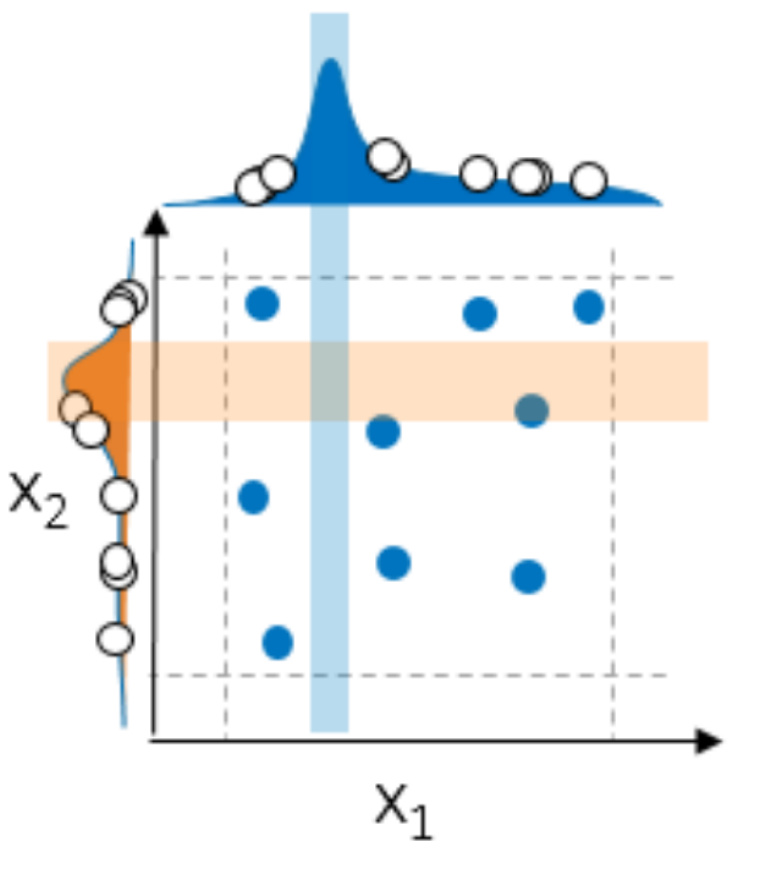
\includegraphics[width=\textwidth]{figures/chp4/random_sampling.png}
        \caption{Random sampling}
    \end{subfigure}
    \begin{subfigure}[t]{.35\textwidth}
        \centering
        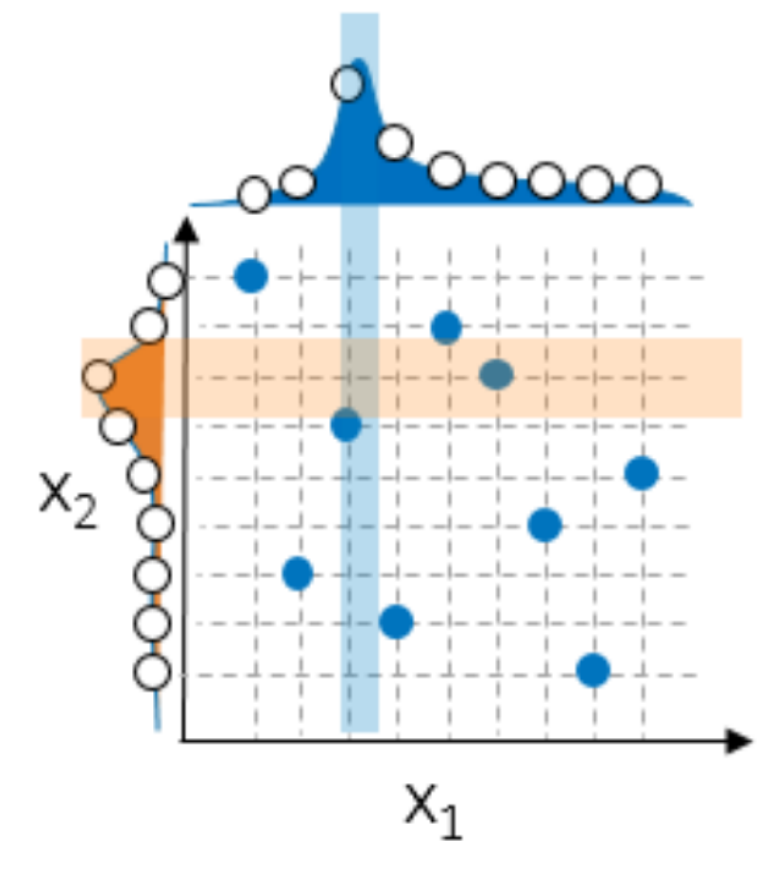
\includegraphics[width=\textwidth]{figures/chp4/latin_hypercube_sampling.png}
        \caption{Latin hypercube sampling}
    \end{subfigure}
    \caption[Random vs Latin hypercube sampling]{Comparison of sampling methods for a Monte Carlo simulation of two variables ($X_1$ and $X_2$) with 9 samples drawn from each. \textbf{a)} Random sampling, where values are drawn at random from each variable's distribution, and \textbf{b)} Latin hypercube sampling, where values are drawn from equal-probability intervals. Note the effective coverage of the distributions in \textbf{b} relative to \textbf{a}. The figure is adapted from \citet{kochautomated2017}.}
    \label{fig:chp4_latin_hypercube_sampling}
\end{figure}

Due to the computational demand of a full inversion workflow, the total number of inversions in each Monte Carlo simulation is limited. To ensure the uncertainty distributions of the inputs are adequately sampled with this limited number of possible runs, we have used Latin hypercube sampling where possible \citep{jansenmonte1994}. This sampling technique is well suited for computationally demanding tasks since it ensures proper coverage of the uncertainty distributions of the sampled values, despite a low number of samples \cite{heltonsurvey2006}. To accomplish this, for a Monte Carlo simulation of $N$ runs, the given distributions are split into $N$ intervals of equal probability and one value is chosen from each interval. The $N$ values for each parameter are then randomly paired to get $N$ sets of sampled input parameter values \citep{heltonsurvey2006}. Since the gravity data and constraint points are each sampled on a point-by-point basis, Latin hypercube sampling is unnecessary and random sampling is used. Figure \ref{fig:chp4_latin_hypercube_sampling} shows a $N=9$ comparison of random sampling and Latin hypercube sampling for a two-parameter simulation. \\


\section[Past inversions]{Relation to past bathymetry inversions\sectionmark{Past inversions}} \label{chp4:past_inversions}

The fundamental theory in all bathymetry inversions is based on the fact that the density contrast across the bathymetry surface produces a measurable gravity effect. This phenomenon gives rise to several techniques to convert observed gravity data into bathymetric depths. This by definition is a geophysical inverse problem \citep{oldenburginversion2005}, but the methods chosen to solve it vary from 3D rigorous inversions to iterative 2D forward modelling. Our inversion method follows a classical least-squares approach to solving the inverse problem, while our uncertainty and sensitivity analysis follows a Bayesian approach \citep{asterparameter2018}. Here, we compare our inversion method and workflow to other bathymetry inversions. We attempt to include all past studies related to Antarctica, as well as several from Greenland. We start by comparing our technique for the gravity reduction process, followed by differences in the actual inversion, and finally by differences in our assessment of uncertainty. \\

\subsection{Gravity reduction comparison}

One of the largest differences between our method and past studies is the gravity reduction process. We employ a rigorous terrain mass effect calculation to obtain a topo-free gravity disturbance, often referred to as a Complete Bouguer Anomaly \citep{vajdasecondary2007}. Theoretically, this gravity signal contains only effects due to subsurface density anomalies and inaccuracies in calculating the terrain mass effect. Our method isolates the gravity effect of this inaccuracy since it is due to the deviations between the starting model of bathymetry and the true bathymetry. This is referred to as our residual component of the topo-free gravity disturbance. While most other bathymetry inversion studies achieve a similar residual anomaly, they complete this procedure in a theoretically different way, which may be introducing unnecessary errors. The differences arise from other studies ignoring the reference surface (the ellipsoid) for all calculations after the normal gravity correction.\\

The sign of a gravity disturbance value informs the interpreter as to whether the true Earth has either excess or deficient mass at that location with respect to the normal Earth. Therefore, the absolute level of gravity disturbance data should be retained, even though direct offsets (DC shifts) don't alter the amplitude of the gravity anomalies. For this reason, the reference surface used in the normal gravity calculation (here the ellipsoid) should be continued to be used in all further calculations of topographic masses, including in the forward calculation made during the inversion, as shown in Figure \ref{fig:chp4_discretized_topo_mass_effect} b. Many studies instead have discretized the ice, water, and starting bathymetry surfaces into prism layers which either have arbitrary references or density values not relative to the normal Earth model. This alternative discretization is shown in Figure \ref{fig:chp4_discretized_topo_mass_effect}f-h. For example, the gravity effect of ice, if not just ignored \citep[e.g.,][]{yangfeasibility2020, cochraninversion2012, jordannew2020, millanbathymetry2017}, is typically removed via a "stripping" technique \citep{vajdaglobal2008}, \citep[e.g.,][]{yangbathymetry2021, millanconstraining2020, mutosubglacial2013,greenbaumocean2015}. This stripping involves calculating the forward gravity of prisms with tops defined by the ice surface, bottoms defined by the ice base, and densities defined by the assumed density of ice (Figure \ref{fig:chp4_discretized_topo_mass_effect}f). Additionally, the prisms which comprise the starting bathymetry model for many inversions are bound above by the starting bathymetry, and below by an arbitrary constant depth (Figure \ref{fig:chp4_discretized_topo_mass_effect}h) \citep[e.g.,][]{mutosubglacial2013, tintoross2019}. The forward gravity calculations of this style of discretization can introduce several errors.
\begin{enumerate}
    \item The largest of these errors is an offset in the mean value of the forward gravity relative to the observed gravity. This offset needs to be estimated and removed prior to comparison with the observed data. The DC-shift used to remove the offset is typically estimated by finding a value that minimizes the difference between the observed and predicted data at locations of known bathymetry \citep[e.g.,][]{boghosianresolving2015, cochrandetailed2020, eisermannbathymetry2020, constantinoseafloor2020, mutosubglacial2013, millanbathymetry2017}. This additional step, referred to as "pinning", is unnecessary in our implementation, due to adhering to a rigorous determination of the terrain mass effect. If an incorrect DC shift is applied, the significance of the zero level of the topo-free gravity disturbance is lost. The value of 0 signifies that the simplified model of the Earth (i.e. the starting bathymetry model) is equal to the true Earth density distribution. Shifting this zero-level due to errors in estimating the DC-shift may lead to a vertical offset in the inverted bathymetry, especially if the inversion domain isn't well constrained. The DC-shifted terrain mass effect and the rigorous terrain mass effect for Antarctica are compared in Figure \ref{fig:chp4_antarctic_topo_free_disturbance}d.
    
    \item The forward gravity calculation with this style of discretization results in slightly different amplitude anomalies compared to the true terrain mass effect. This difference is due to the different densities assigned to the prism layer between the two techniques (Figure \ref{fig:chp4_discretized_topo_mass_effect}). While this difference is likely below the range of uncertainties in the gravity error, it is an unnecessary addition of error to the gravity reduction process.
    
    \item The last drawback to using this alternative discretization is an increased gravitational edge effect. As shown in Figure \ref{fig:chp4_discretized_topo_mass_effect}, the average densities and prism heights are larger with this technique. This increases the overall decay of calculated gravity at the edges of the model space, due to the contrast with the void-space beyond the model domain. To account for this, a larger buffer zone is needed, which can significantly increase the computational requirements during forward modelling (see Chapter \ref{ch:3} Section \ref{chp3_edge_effects}).
\end{enumerate}

\subsubsection{Regional separation}
The last step in the gravity reduction process for bathymetry inversion is separating the regional and residual signals, where the residual signal should theoretically be entirely a result of the bathymetry surface. Some techniques commonly used for this are described in Chapter \ref{ch:3} Section \ref{chp3_regional_seperation}. Past bathymetry inversions have used a variety of these techniques, as summarized below.

\begin{enumerate}
    \item Zero or uniform adjustment; For small inversion domains the regional field is sometimes assumed to be minimal. In these scenarios, past studies have either limited the inversion domain to where the regional field is assumed small \citep{cochraninversion2012, boghosianresolving2015}, used a uniform value for the regional component \citep{mutobathymetry2013}, or found a constant density value for the starting model which minimize the gravity misfit \citep{millanvulnerability2018, millanbathymetry2017, anbed2017}.
    
    \item Low-pass filtering; for inversion domains with an expected regional field slightly larger than the above scenario, low-pass filtering of the gravity data can approximate the regional component \citep{eisermannbathymetry2020, hodgsonfuture2019}. 
    
    \item Geologic modelling; To account for the regional field, some studies create geologic models of varying density to estimate the regional field. These models are typically informed from other geophysical data \citep{hodgsonfuture2019, greenbaumocean2015}, \textit{a priori} geologic knowledge \citep{tintoprogressive2011, cochranbathymetric2014, constantinoseafloor2020}, or from an approximated crustal density distribution \citep{tintoross2019, cochrandetailed2020, eisermannbathymetric2021, weigetz2020}.
    
    \item Upwards continuation / high altitude surveys; This technique estimates the long-wavelength regional component by either upward continuing the gravity data to large altitudes, using separate gravity data collect from high-altitude surveys \citep{mutosubglacial2016}, or a combination of both \citep{tintobathymetry2015}
    
    \item Constraint point minimization; the last commonly used technique utilizes the assumption that the desired residual component is near-zero at points of known bathymetry. From this assumption, the regional component at these constraint points is entirely equal to the gravity anomaly value. To estimate the regional field, the gravity values are sampled at the constraint points and interpolated over the region. This technique has been used in several recent inversions where sparse constraint points are available \citep{millanconstraining2020, yangbathymetry2021, yangocean2020, anbathymetry2019, anbathymetry2019a, jordannew2020, vaňkováhigh2023}. While implemented in a different method, this constraint point minimization follows the same concept as several studies which use the constrained locations to derive a spatially variable density model, accounting for the regional field \citep{tintoross2019, eisermannbathymetric2021, weigetz2020}.
\end{enumerate}

Here, we use the constraint point minimization technique for estimating and removing the regional component of the topo-free gravity disturbance.

\subsection{Inversion comparison}

We have developed a conventional non-linear geometric gravity inversion algorithm, as often used in modelling density contrasts, such as sedimentary basins \citep[e.g.,][]{martinssimultaneous2010, santosefficient2015}, or the Moho \citep[e.g.,][]{uiedafast2017, pappamoho2019}. This algorithm is similar in concept to inversions used in other bathymetric studies but differs in its implementation. Past inversion techniques used for bathymetry modelling can be grouped into several categories;
\begin{enumerate}
    \item algorithmic approaches. This method termed the "topographic shift method" \citep{hodgsonfuture2019, jordannew2020}, while not a formal inversion, calculates the equivalent rock thickness from the residual component of gravity, adds this to the starting bathymetry model, and constrains the results by the locations of known bathymetry.
    
    \item 2D profile inversions. Using the method of \citet{talwanirapid1959}, and often implemented within the commercial software Geosoft Oasis Montaj, these inversions retain the 2D nature of the airborne flight lines and invert only along the path of the flight \citep{tintobathymetry2015, cochranbathymetric2014, weigetz2020, boghosianresolving2015, cochrandetailed2020, tintoprogressive2011, constantinocook2023}.
    
    \item 3D frequency-based inversions. This category of inversion uses a Fourier transformation to calculate the forward gravity effect of a continuous topographic surface, forgoing the need to discretize the topography into vertical prisms \citep{parkerrapid1972, oldenburginversion1974}. This Fourier transform is then iteratively modified to minimize the misfit to the observed gravity. This method, particularly its implementation within the commercial software Geosoft Oasis Montaj, is frequently used for bathymetry inversions \citep{anbathymetry2019a, anbathymetry2019, anbed2017, greenbaumocean2015, millanconstraining2020, eisermannbathymetry2020, cochraninversion2012, millanvulnerability2018, millanbathymetry2017, studingerestimating2004, eisermannbathymetric2021}.
    
    \item Simulated Annealing. This global optimization technique \citep{kirkpatrickoptimization1983} performs many forward calculations of possible bathymetry surfaces and slowly converges on a model which minimizes the misfit with the observations. This method, similar to our Monte Carlo uncertainty analysis, has the benefit of providing an uncertainty estimate of the resulting bathymetry based on the uncertainty in the inversion inputs. This has been used in several bathymetric inversions \citep{royinversion2005, mutosubglacial2013, mutosubglacial2016, yangocean2020, yangbathymetry2021, yangseafloor2018, filinanew2008}

    \item Regularized least-squares inversions. This style of inversion is the conventional approach to solving non-unique inverse problems \citep{asterparameter2018}. While this method is commonly used for other geometric gravity inversions (e.g., Moho and basement), to our knowledge it is only applied to bathymetry inversions here, and in \citet{vaňkováhigh2023}.
\end{enumerate}

\subsection{Uncertainty comparison}

Here we compare our uncertainty analysis to those from other bathymetry-gravity inversion studies. Most of these past studies provide an estimation of uncertainty, but only a few provide spatially variable uncertainties \citep[e.g.,][]{anbathymetry2019, mutosubglacial2016}. Typically, these inversion uncertainties are assumed to result from three sources.

\begin{enumerate}
    \item Uncertainty in the gravity data. The uncertainties resulting from the gravity data uncertainty are typically estimated using a Bouguer slab approximation, with an assumed density of the contrast between rock and water ($\sim$~1600~kg~m\textsuperscript{-3}), and a gravity uncertainty approximated from the RMS crossover values of the airborne gravity survey \citep[e.g.,][]{tintoross2019, constantinoseafloor2020, boghosianresolving2015}. Alternatively, a simple conversion factor has been proposed of 100~m of inversion uncertainty per 5~mGal of gravity uncertainty \citep{anbathymetry2019, anbathymetry2019a}.

    \item Assumptions of the geologic structure. The uncertainty resulting from assumptions of the geologic structure is typically simplified as uncertainties in the choice of the constant density contrast between sediment and seawater. This uncertainty is sometimes approximated as a ratio of change in density to change in inverted relief as a percentage \citep[e.g., $\sim$3\% relief for 50~kg~m\textsuperscript{-3}][]{tintoross2019} or by altering the density and comparing the results \citep{boghosianresolving2015}.

    \item Uncertainties in the past measurements of bathymetry (constraints). Lastly, constraint point measurement uncertainties are typically assumed to result in a 1:1 uncertainty in the inverted bathymetry \citep[e.g.,][]{tintoross2019, boghosianresolving2015}.
\end{enumerate}

Our uncertainty analysis, through Monte Carlo simulation, provides robust spatial uncertainty estimates for each of these three sources of uncertainty. Similar to the above methods, Monte Carlo simulation only addresses uncertainties related to the uncertainty of the inputs to the inversion.

\section{Results}

Here we apply the above-described methods to recover a higher resolution bathymetry beneath Antarctica's Ross Ice Shelf. First, we show the results from an individual workflow, as depicted in Figure \ref{fig:chp4_workflow}. This includes the starting bathymetry model, the topo-free gravity disturbance calculations, and the resulting inverted bathymetry. Next, we present the Monte Carlo simulation results, where this entire workflow is repeated many times with varying values of input data and parameters.\\

\subsection{Starting bathymetry}

Existing options for a starting bathymetry model for the sub-Ross Ice Shelf include Bedmap2 \citep{fretwellbedmap22013} or BedMachine v3 \citep{morlighemdeep2020, morlighemmeasures2022}. BedMachine v3 for the Ross Ice Shelf contains the gravity-inverted bathymetry results from \citet{tintoross2019}. To avoid over-interpretation of the gravity data (starting an inversion with the results of a separate inversion) we opted to not use BedMachine for the starting model. Bedmap2 bed elevations for the Ross Ice Shelf were created through the interpolation of the point constraints \citep{fretwellbedmap22013}. These point constraints within the ice shelf (Figure \ref{fig:chp4_inversion_inputs}b) were compiled from several surveys, including the early traverses of the 1950s and 60s \citep{craryglaciological1962,  craryoversnow1959,craryoversnow1962}\footnote{These surveys included the Ross Ice Shelf Traverse (1957-1958), the Little America Station Byrd Trail Traverse (1958), the Victoria Land Traverse (1958-1959), and the Discovery Deep Traverse (1960), see \citet{bennettgravity1964} for the data and descriptions.}, and the Ross Ice Shelf Geophysical and Glaciological Survey \citep[RIGGS, 1973-1974][]{bentleyross1984} ($N=223$). However, the gridding algorithm used (ArcGIS Topogrid), while producing smooth results for the Ross Ice Shelf, didn't strictly adhere to the constraint point depths. This can be seen through the comparison of constraint point depths and Bedmap2 grid values at the same location (Figure \ref{fig:chp4_inversion_inputs}b). The RMS difference between the constraint depths and the grid depths within the ice shelf is 138~m. The largest differences are concentrated along the Transantarctic Mountain Front, where Bedmap2 grid values are much shallower than the constraint points. Due to this over-smoothing of the constraints, we have opted to create our own starting bathymetry model.\\

Our starting model was created from the combination of various seismic survey constraint points on the ice shelf, and bed data from BedMachine v3 \citep{morlighemdeep2020, morlighemmeasures2022} outside of the ice shelf. To create this, the BedMachine v3 bed elevations, relative to the WGS-84 ellipsoid, were masked within the Ross Ice Shelf, based on the MEaSUREs v2 Ross Ice Shelf boundary \citep{mouginotmeasures2017, rignoticeshelf2013}. These data were converted from gridded data into point data and merged with the various bathymetry data within the ice shelf. A continuous grid of bathymetry depths at a 5~km cell size was then interpolated from the combined data inside and outside the shelf. The interpolation can be accomplished with two gridding methods, bi-harmonic splines \citep{sandwellbiharmonic1987}, and minimum curvature \citep{smithgridding1990}. While the bi-harmonic spline method appears to have several advantages over minimum curvature (Chapter \ref{ch:3} Section \ref{chp3_gridding_comparison}), such as the ability to apply weights to the data, interpolating the above Ross Ice Shelf data resulted in significant unconstrained minima and maxima. Initial inversion results showed these erroneous features carry through to the final inverted bathymetry. Due to this, we have opted to interpolate the data to create the starting bathymetry model using tensioned minimum curvature. This method resulted in less extreme un-constrained minima and maxima.\\

% Both of these methods contain a parameter that must be chosen. For the minimum curvature method, this parameter is the tension factor (Section \ref{chp3_gridding_comparison}), which ranges from 0 to 1. For bi-harmonic splines, the parameter is a damping value applied to the interpolation. This damping is necessary in order to for the interpolation to account for the differing uncertainties of each constraint point \citep{uiedaverde2018}. This avoids an interpolation bias to highly uncertain data. Points outside of the ice shelf were assigned a constant uncertainty of 10 m, reflecting the relatively low uncertainty in determining bed elevation over grounded ice, or open ocean. Points within the ice shelf were assigned uncertainties of 5\% of their depth from the ice surface, equating to a mean uncertainty of 34 m. \\

\begin{figure}[!ht]
    \centering
    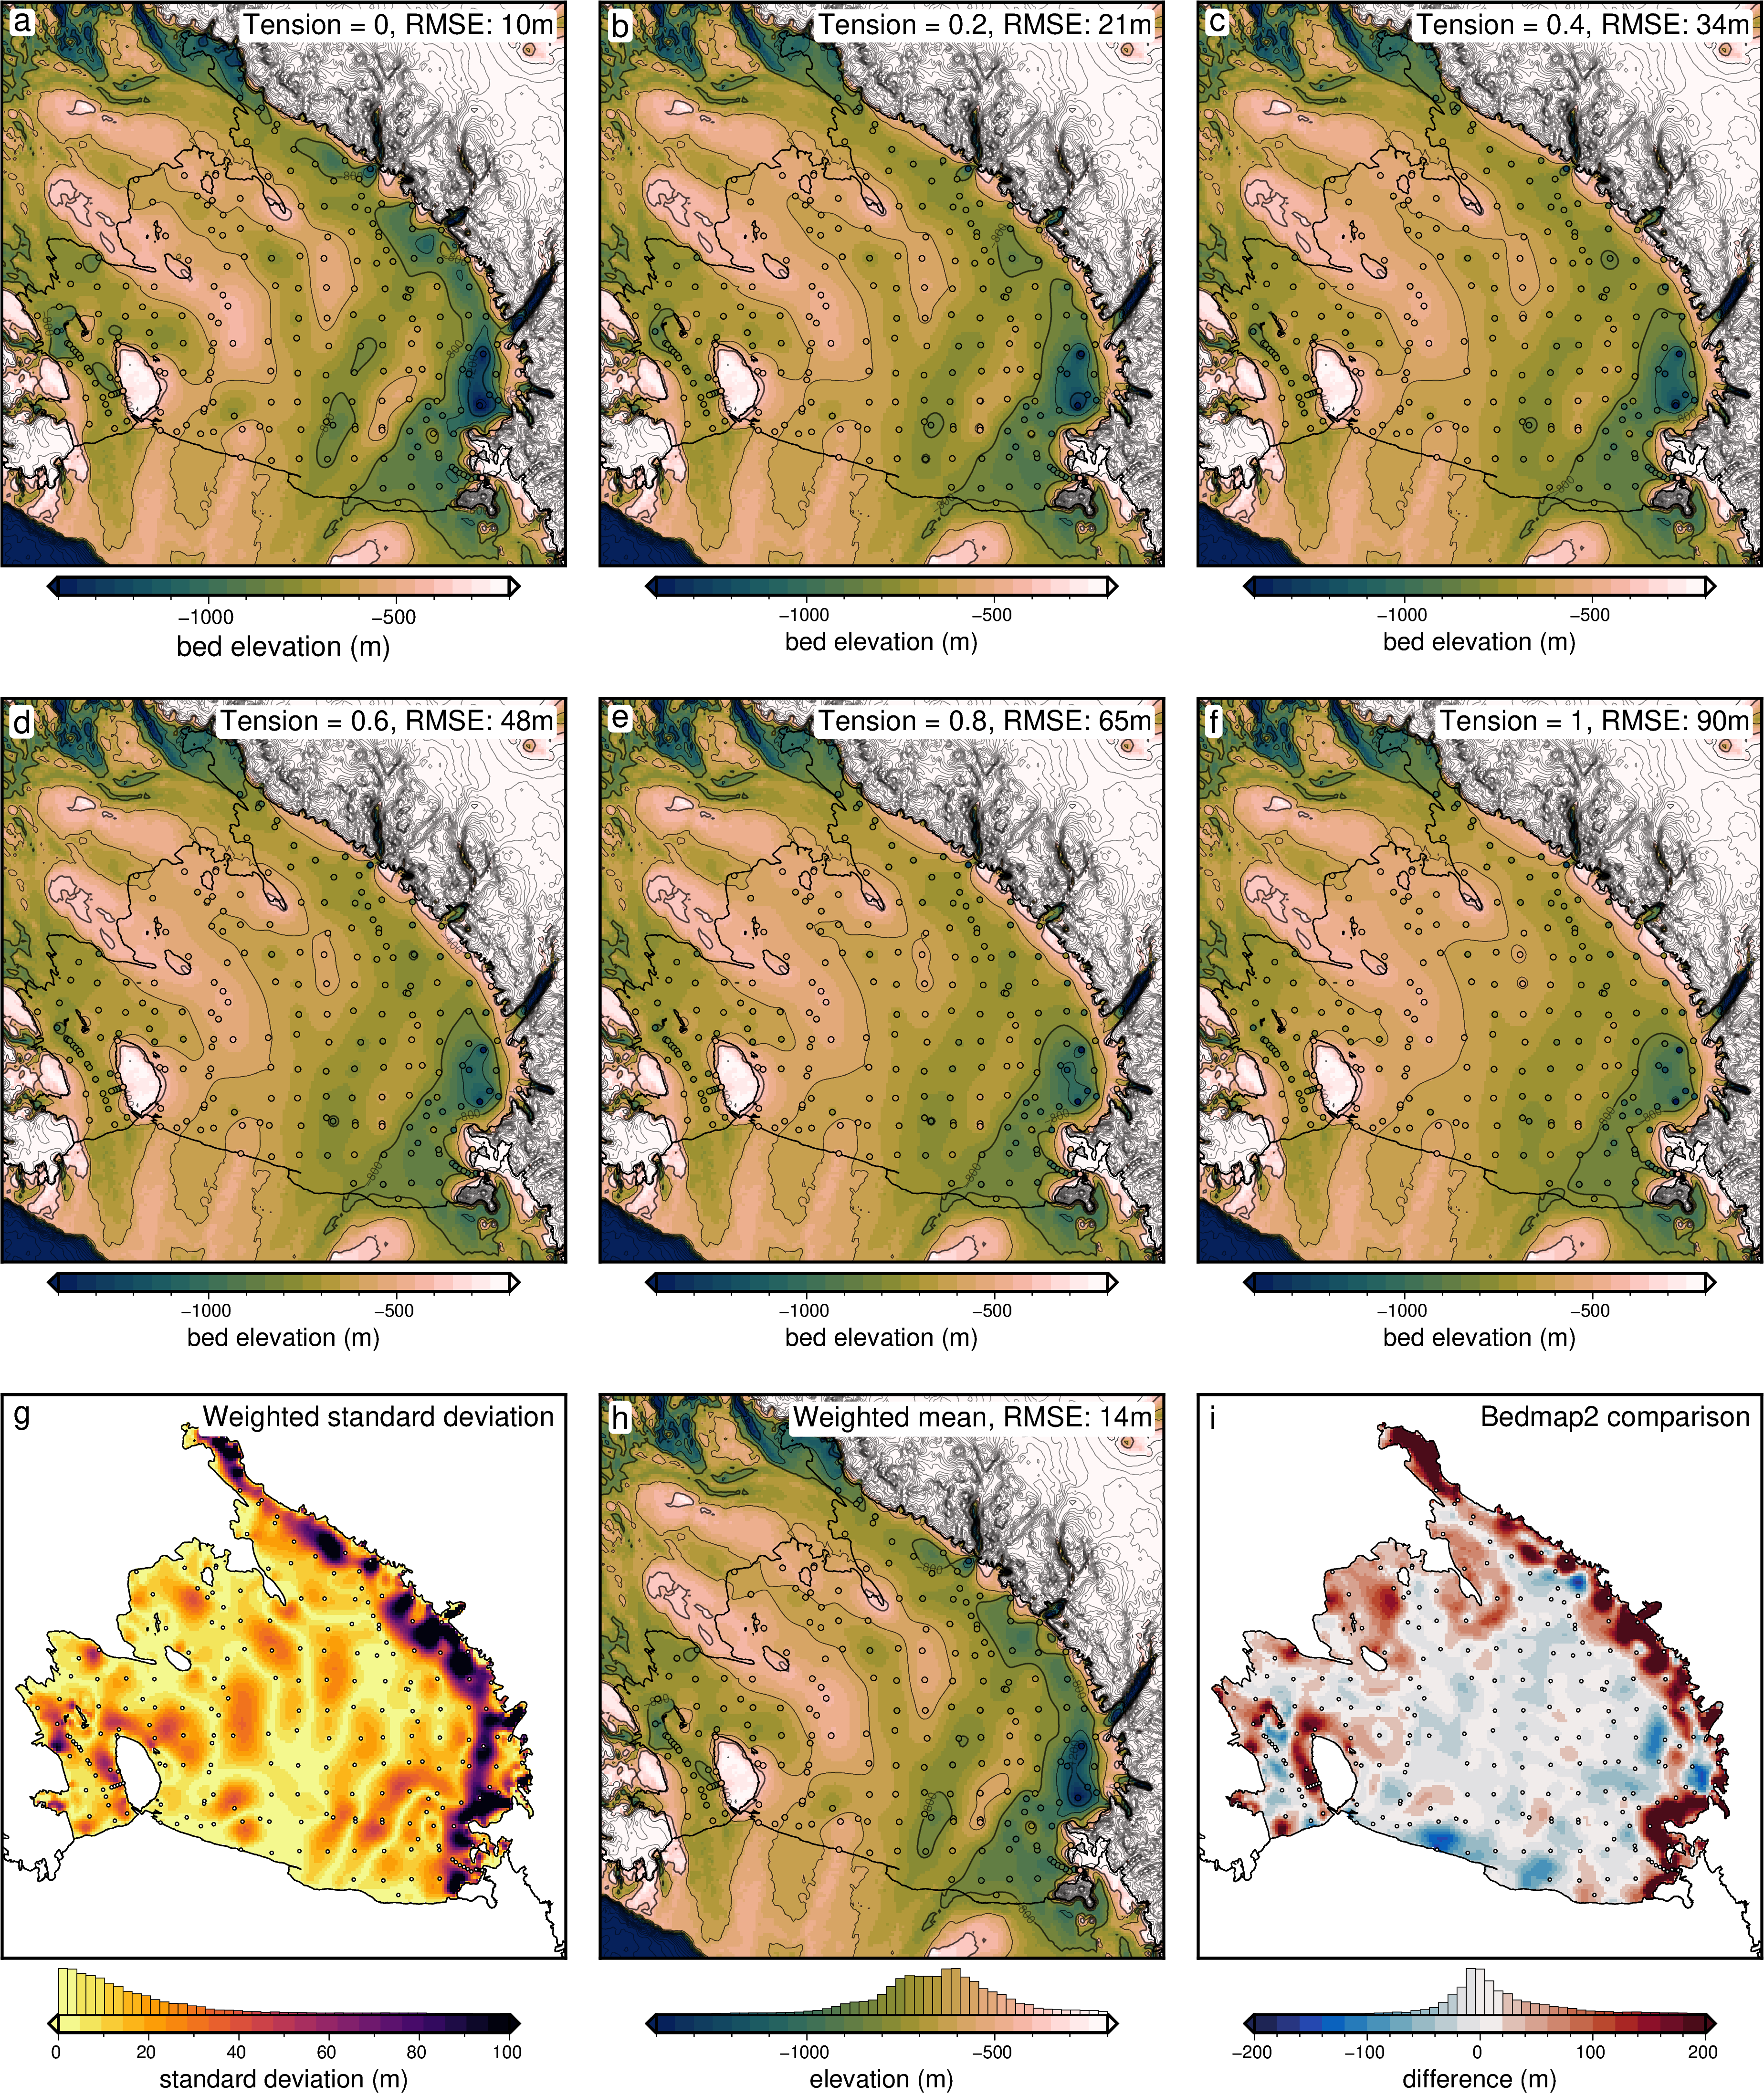
\includegraphics[width=0.98\textwidth]{figures/chp4/starting_bed_comparison.png}
    \caption[Ross Ice Shelf starting bathymetry]{Starting bathymetry models from the interpolation of constraint points within the ice shelf and BedMachine v3 gridded data outside of the shelf \citep{morlighemdeep2020, morlighemmeasures2022}. The ice shelf border, from \citet{mouginotmeasures2017}, is shown as the solid black line, representing the grounding line and the calving front. \textbf{a-f)} Bathymetry models resulting from 6 varying tension factor values of minimum curvature interpolation. Contours shown at 400~m intervals. \textbf{g)} The cell-specific weighted standard deviation of the six models (\textbf{a-f}). \textbf{h)} The cell-specific weighted mean bed elevation from the six models. \textbf{i)} The difference between Bedmap2 bathymetry and the mean model (\textbf{h}). The RMS difference is 95~m. Blues show where the mean model is shallower than Bedmap2, while reds show where the mean model is deeper. Root mean square error (RMSE) values in the plot titles are between the constraint point depths and the values at those points on the interpolated grids.}
    \label{fig:chp4_starting_bed_comparison}
\end{figure}

To test the importance of the tension value used in the minimum curvature gridding, we performed 6 interpolations, with tension values of 0, 0.2, 0.4, 0.6, 0.8, and 1 (Figure \ref{fig:chp4_starting_bed_comparison}a-f). From these six resulting bathymetry models, we calculated the standard deviation (Figure \ref{fig:chp4_starting_bed_comparison}g) and the cell-specific mean (Figure \ref{fig:chp4_starting_bed_comparison}h). These statistics were weighted, in the same method described in Figure \ref{fig:chp4_Monte_Carlo_workflow}d. The weight value used for each grid was the inverse square of the RMS difference between the constraint point depth values and the resulting grid values at the same points. These RMS values are shown in the figure titles of Figure \ref{fig:chp4_starting_bed_comparison}a-f. This weighted mean starting model is compared to Bedmap2 bathymetry (Figure \ref{fig:chp4_starting_bed_comparison}i). Note that while low tension factors result in models that closely match the constraints, they also produce local maxima and minima away from the data, which is not ideal since these features can be seen to carry through the inversion to the final bathymetry, as discussed later. Alternatively, higher tension values produce models that don't match the constraints as well (higher RMS values), but they don't have as many erroneous features. For this reason, we use the cell-specific mean of the six models as our starting bathymetry (Figure \ref{fig:chp4_starting_bed_comparison}h). This model has an RMS difference from BedMap2 within the ice shelf of 95~m.\\

\begin{figure}[!ht]
    \centering
    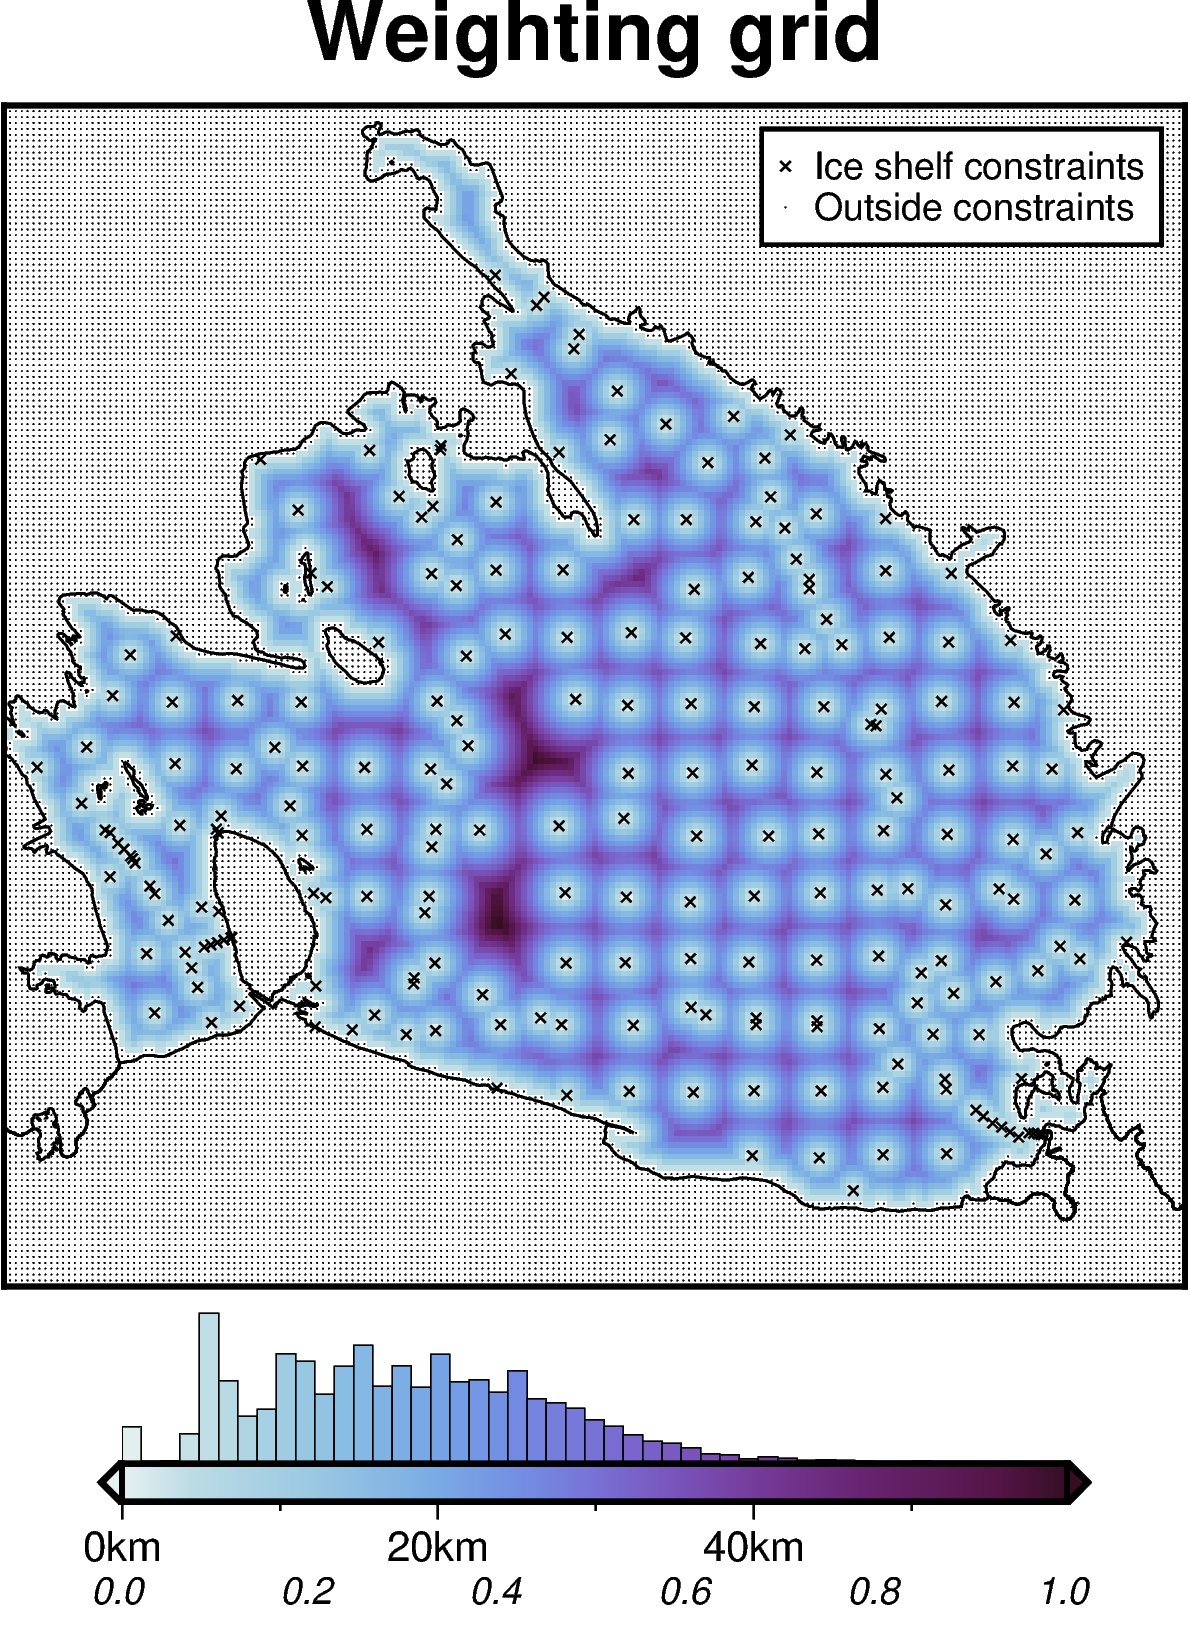
\includegraphics[width=0.5\textwidth]{figures/chp4/RIS_weighting_grid.png}
    \caption[Ross Ice Shelf weighting grid]{Weighting grid used in the Ross Ice Shelf bathymetry inversion. Grid colours show both the distance between each grid cell and the nearest constraint point and the weight values (0 - 1) from the normalization of these distances. Constraint points are defined as either direct measurements of bathymetry within the ice shelf (black crosses), or any grid cell outside of the ice shelf (small black dots). The ice shelf border, from \citet{mouginotmeasures2017} is shown as the solid black line, representing the grounding line or the calving front.}
    \label{fig:chp4_RIS_weighting_grid}
\end{figure}

From these constraint points used to create the starting bathymetry, a weighting grid was created (Figure \ref{fig:chp4_RIS_weighting_grid}). This grid was calculated from the distance between each grid cell and the nearest constraint point. This minimum constraint distance (top annotations of Figure \ref{fig:chp4_RIS_weighting_grid} colourbar) was then normalized between 0 and 1 to create the weighting grid (bottom annotations of Figure \ref{fig:chp4_RIS_weighting_grid} colourbar). As all grid cells outside of the ice shelf border are considered constraint points non-zero weights and  minimum constraint distances are confined to within the ice shelf border. The colourbar histogram shows a mean minimum constraint distance within the ice shelf of approximately 20~km, and an upper limit of approximately 60~km. Within the shelf, there are 223 constraint points. Over an area of $\sim$480,000~km\textsuperscript{2} \citep{mouginotmeasures2017}, this equates to a constraint density of $\sim$1 constraint per $46\times46$~km (2154~km\textsuperscript{2}).\\


\subsection{Gravity processing results} \label{chp4_gravity_processing_results}

We use airborne gravity data from the Ross Ocean and ice Shelf Environment, and Tectonic setting Through Aerogeophysical surveys and modelling project (ROSETTA-Ice). This project was created with the goal of investigating the interactions between ice, ocean, and earth of Antarctica's Ross Ice Shelf \citep{tintoross2019}. The survey consisted of 3 field seasons (2015-2017) of airborne geophysical surveying with a survey design consisting of E-W flight lines, at a nominal spacing of 10~km, and N-S tie lines with a nominal spacing of 55~km (Figure \ref{fig:chp4_inversion_inputs}a). Flights were flown at an average of 750~m above the ice surface and a speed of 180~knots (93~ms\textsuperscript{-1}), The survey was designed to maximize the overlap between the flight lines and the past bathymetry constraints across the ice shelf from the RIGGS seismic surveys \citep{bentleyross1984}. The data collection and initial processing were performed by \citet{tintoross2019} and are briefly summarized here. The gravity data were collected with a combination of a LaCoste and Romberg gravimeter upgraded with a ZLS UltraSys control system, an iMAR inertial measurement unit, and a DgS gravimeter. The ZLS data were tied to an absolute gravity reference station at McMurdo Station. Poor-quality data from the ZLS were replaced with the iMAR or DgS values. The accelerations of the aircraft were calculated from GPS data and removed from the gravity signal. The E\"{o}tv\"{o}s correction was applied, to account for measuring gravity on a moving platform \citep{harlaneotvos1968}. At each observation point, the effects of the normal earth were calculated and removed, giving the gravity disturbance values (See Section \ref{ch4 normal gravity}). Levelling was then performed using the cross-over values between E-W flight lines and N-S tie lines.\\

\begin{figure}[!ht]
    \centering
    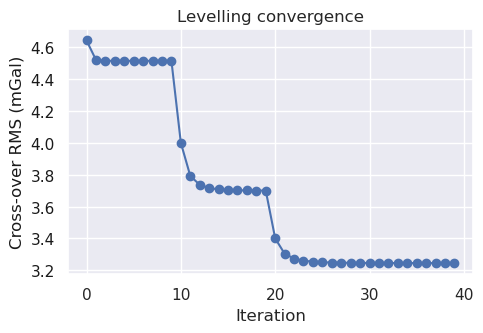
\includegraphics[width=0.6\textwidth]{figures/chp4/ROSETTA_levelling_convergence.png}
    \caption[Re-levelling of the ROSETTA-Ice gravity data]{Re-levelling of the ROSETTA-Ice gravity data. First, flight lines were individually upward continued, then cross-over point misties were found. These were used in 0\textsuperscript{th}, 1\textsuperscript{st}, and 2\textsuperscript{nd} order iterative levelling, alternative between levelling flight lines to tie lines and vice versa at each iteration. The RMS cross-over errors at each iteration are shown. The major steps show the 0\textsuperscript{th}, 1\textsuperscript{st}, and 2\textsuperscript{nd} order stages of levelling.}
    \label{fig:chp4_levelling}
\end{figure}

Since this bathymetry inversion is strongly influenced by noise in the gravity data, as demonstrated in Chapter \ref{ch:3} Section \ref{chp3_effect_of_gravity_noise}, we have performed additional processing to the published ROSETTA-Ice dataset. Erroneous sections of flight line data were manually removed, and the dataset was re-levelled. The levelling procedure utilizes the gravity difference between E-W and N-S flight lines at cross-over points. While the flight paths intersect in 2-D space, their altitudes typically differ, meaning there is no true cross-over point in 3-D space. To account for this, the flight lines are individually upward continued to a constant elevation of 1~km (ellipsoidal height). The mean elevation of the cleaned data was $\sim$790~m, and 1~km was greater than 96\% of the data. This limited the amount of downward continuation while retaining a spatial resolution close to the original data. This continuation was calculated using the equivalent source technique \citep[see Section \ref{chp3:eq source resampled}][]{dampneyequivalent1969, solergradientboosted2021}. Since the cross-over points are now true 3-D intersections, the difference between E-W and N-S lines at these points (mis-ties) can be used to re-level the dataset. Here, we alternate between levelling the E-W lines to the N-S lines, and vice versa. We start with a 0\textsuperscript{th} order levelling, where only DC shifts are applied. Followed by a 1\textsuperscript{st} and 2\textsuperscript{nd} order levelling, where 1 and 2-degree polynomials, respectively, are fit to the mis-ties, and used to level the lines. The results of this levelling procedure are shown in Figure \ref{fig:chp4_levelling}. For each order of levelling several iterations are performed. The step-wise convergence of the RMS mis-tie values shows the 0\textsuperscript{th}, 1\textsuperscript{st}, and 2\textsuperscript{nd} order levelling stages. The re-levelling procedure brought the RMS mis-tie from $\sim$4.8~mGal to $\sim$3.2~mGal. \\

Finally, this re-levelled gravity disturbance line data were gridded onto a regular grid at 2.5~km spacing, using equivalent sources. Since the inversion only affects the bathymetry within the ice shelf border, as implemented with the weighting grid (Figure \ref{fig:chp4_RIS_weighting_grid}), the interpolated gravity grid is masked beyond 10~km outside of the ice shelf border (Figure \ref{fig:chp4_levelling}b). This 2.5~km gridded data ($N=85,914$) consists of both the \textit{testing} ($N=64,435$) and \textit{training} ($N=21,479$) sets used in the cross-validation. With the grid configuration shown in Chapter \ref{ch:3} Figure \ref{fig:chp3_CV_grid_spacing}, the \textit{training} data used in the actual inversion are on a regular 5~km grid. \\

\subsection{Gravity reduction results}

The terrain mass effect was calculated at each of the gridded gravity data points. For this calculation, the three layers of prisms shown in Figure \ref{fig:chp4_discretized_topo_mass_effect}c-e were created from BedMachine v3 \citep{morlighemdeep2020, morlighemmeasures2022} ice surface and water surface data and the mean starting bathymetry from Figure \ref{fig:chp4_starting_bed_comparison}h. All data are referenced to the WGS-84 ellipsoid. The ice surface elevations used from BedMachine v3 are in ice equivalent, meaning they have had a firn depth correction applied, making for a slightly lower surface elevation to account for spatially variable firn thickness \citep{morlighemdeep2020}. An ice equivalent surface is suitable for calculating the terrain mass effect since it gives the estimated thickness of the ice shelf with a density of ice, instead of the true ice shelf thickness, with a layer of low-density firn above. Comparing the forward gravity calculated from the true geometry of ice shelf thickness, the ice equivalent thickness, and a 2-layer model with firn and ice, show minimal differences, and thus we use the ice equivalent thickness in the terrain mass effect. The densities used in the terrain mass effect calculations were 1~kg~m\textsuperscript{-3} for air, 915~kg~m\textsuperscript{-3} for ice, 1024~kg~m\textsuperscript{-3} for seawater \citep{griggsantarctic2011}, and 2300~kg~m\textsuperscript{-3} for seafloor. Since we use a single value for the density of the seafloor, it should represent the expected average density of the seafloor over the entire region. Chapter \ref{ch:2} showed a continuous drape of sediment over the seafloor. We chose 2300 kg m\textsuperscript{-3} to be in the middle between unconsolidated sediment ($\sim1900$~kg m\textsuperscript{-3}) and low-density crystalline rock ($\sim2700$~kg m\textsuperscript{-3}) \citep{schöndensity2015}. The inversion domain was 1 million km\textsuperscript{2} (1000~km~$\times$~1000~km). To avoid gravitational edge effects in the forward calculations, the prism layers were extended in all directions by a 40~km buffer zone, resulting in 120,000 prisms. The resulting terrain mass effect was subtracted from the gravity disturbance to get the topo-free gravity disturbance. These data are shown in Figure \ref{fig:chp4_RIS_terrain_regional_residual}.\\

\begin{figure}[!ht]
  \centering
    \begin{subfigure}[t]{.99\textwidth}
        \centering
        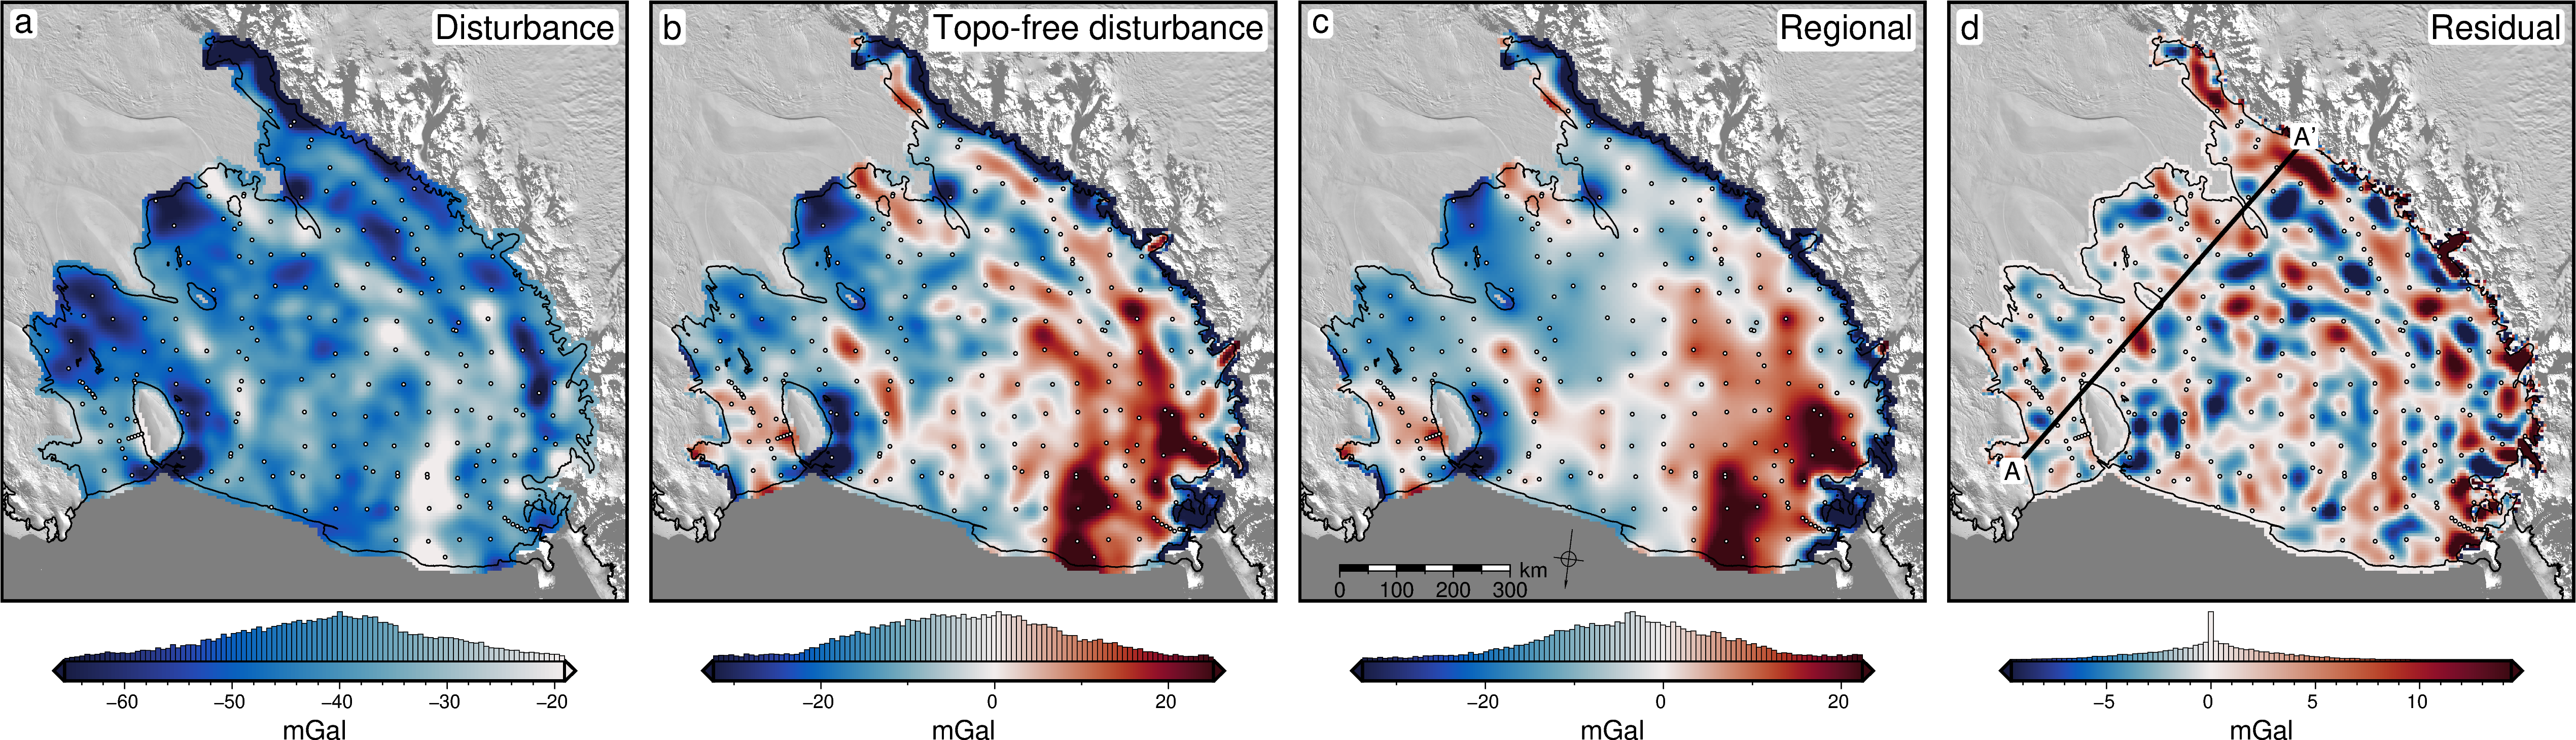
\includegraphics[width=\textwidth]{figures/chp4/RIS_terrain_regional.png}
    \end{subfigure}
    \begin{subfigure}[t]{.8\textwidth}
        \addtocounter{subfigure}{4}
        \centering
        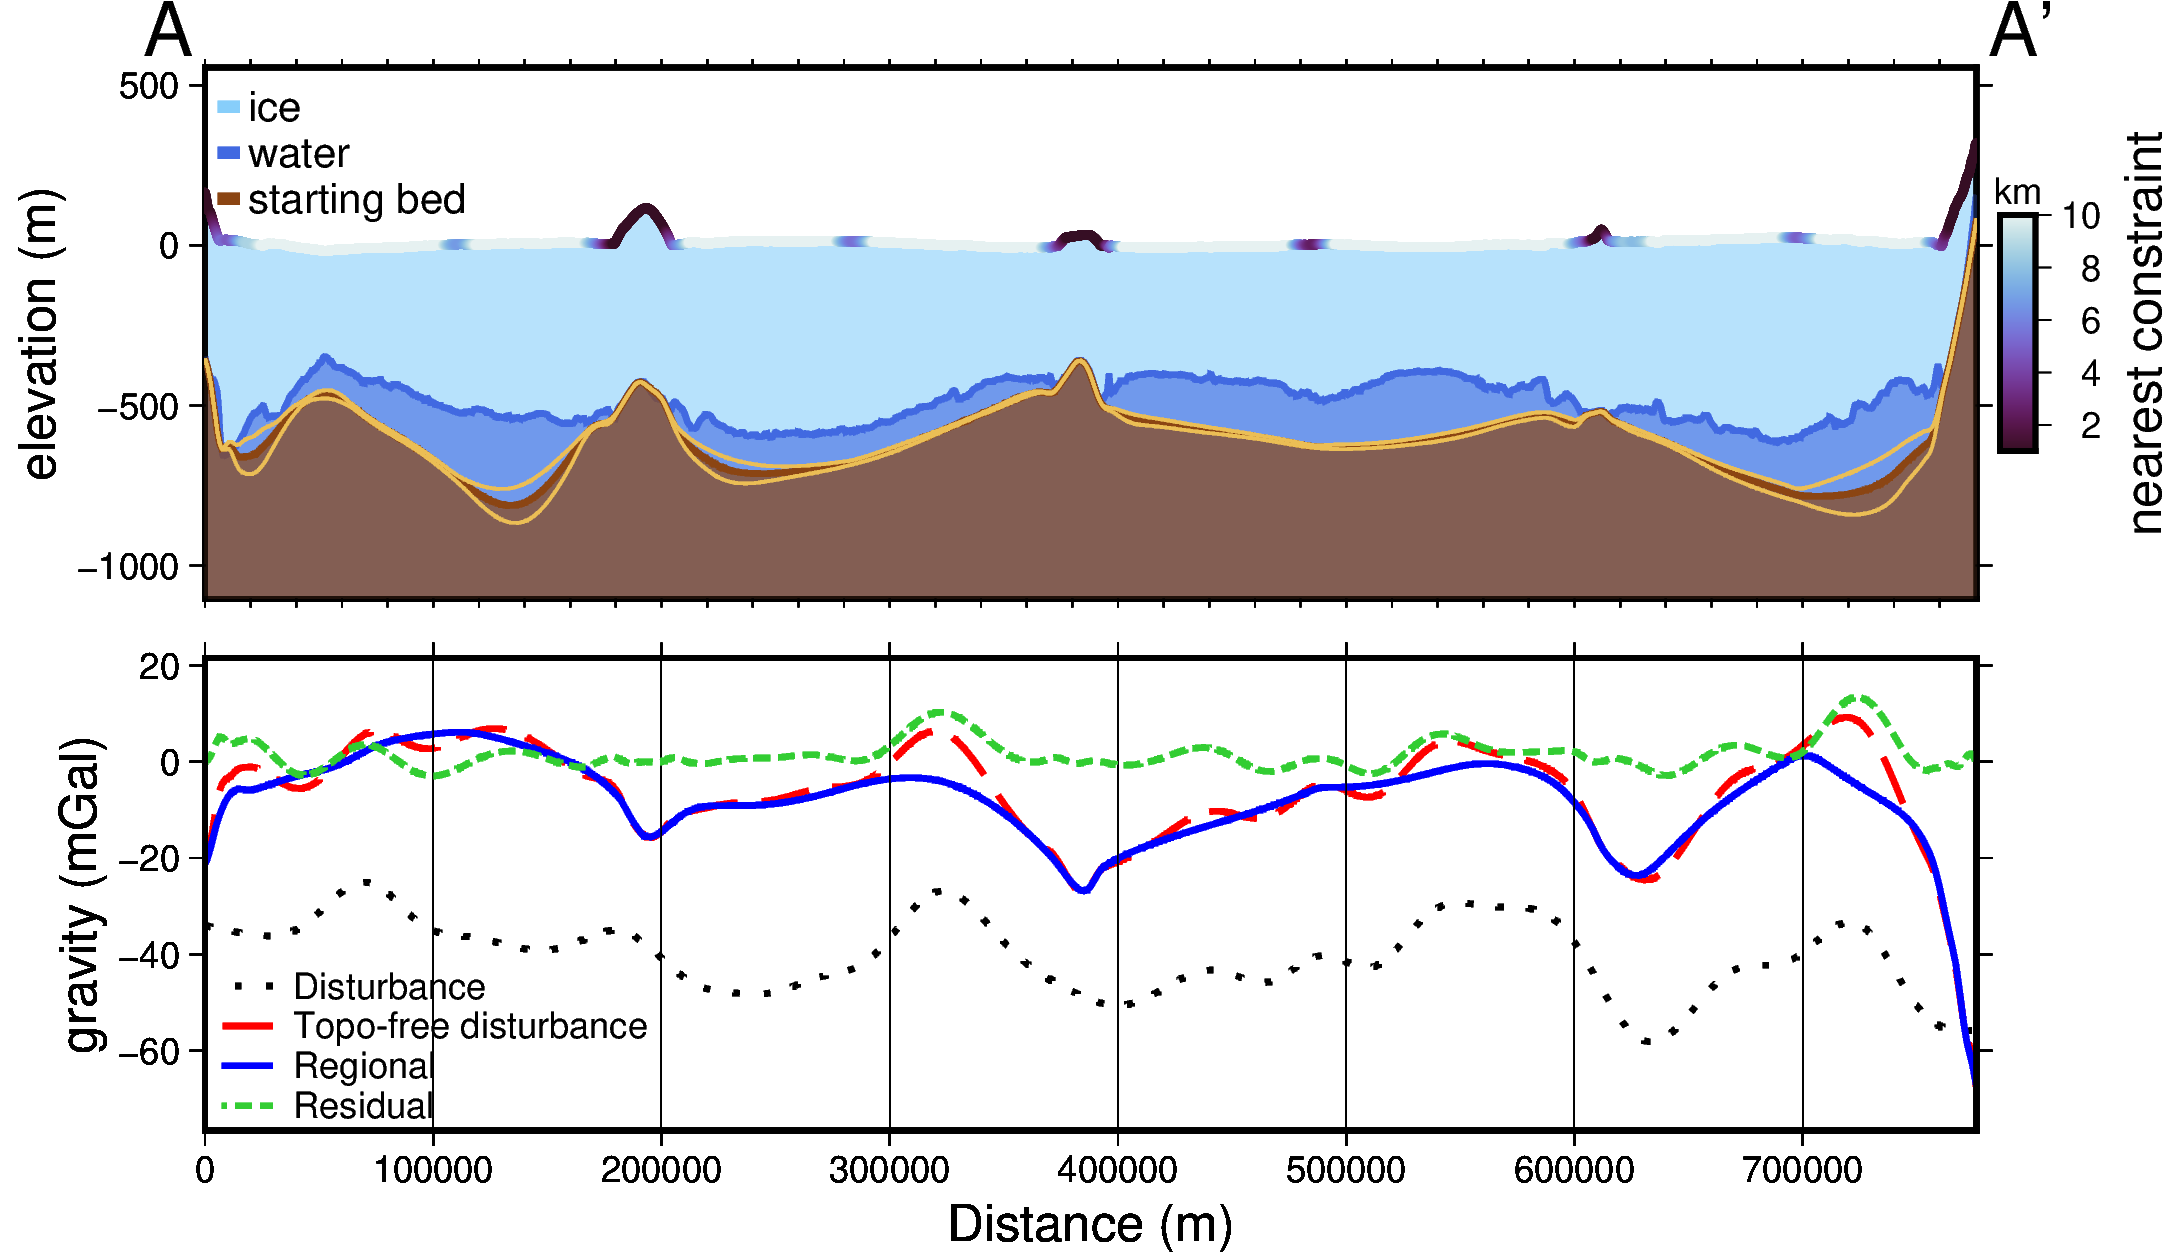
\includegraphics[width=\textwidth]{figures/chp4/RIS_terrain_regional_profile.png}
        \caption{}
    \end{subfigure}
  \caption[Gravity reduction results for the Ross Ice Shelf]{Gravity reduction results for the Ross Ice Shelf. \textbf{a)} Gravity disturbance, \textbf{b)} topo-free gravity disturbance, after the removal of the terrain mass effect, \textbf{c)} regional component of the topo-free disturbance, estimated with constraint point minimization, and \textbf{d)} residual component of the topo-free disturbance, as the difference between \textbf{b} and \textbf{c}. Background imagery is from MODIS-MOA \citep{scambosmodisbased2007} and grounding line and coastlines are from \citep{morlighemmeasures2022}. Constraint points within the ice shelf are shown as dots. \textbf{e)} Profile from A to A', location shown in \textbf{d}. \textbf{Upper panel} shows cross-section, with ice surface and ice base from BedMachine v3 \citep{morlighemdeep2020, morlighemmeasures2022}. Brown layer shows the mean starting bed model with bounding uncertainty (light brown lines) from the standard deviation of the various starting bed models in Figure \ref{fig:chp4_starting_bed_comparison}. The colour of ice surface shows the distance to the nearest constraint point. \textbf{Lower panel} shows data from \textbf{a-d} along the profile.}
    \label{fig:chp4_RIS_terrain_regional_residual}
\end{figure}

% \begin{figure}[!ht]
%   \centering
%     \begin{subfigure}[t]{.95\textwidth}
%         \centering
%         \includegraphics[width=\textwidth]{figures/chp4/RIS_terrain_effects.png}
%     \end{subfigure}
%     \begin{subfigure}[t]{.8\textwidth}
%         \addtocounter{subfigure}{3}
%         \centering
%         \includegraphics[width=\textwidth]{figures/chp4/RIS_terrain_effects_profile.png}
%         \caption{}
%     \end{subfigure}
%   \caption{Terrain mass effect correction. \textbf{a)} Forward calculated terrain mass effect from of BedMachine v3 ice surface, water surface, and the mean starting bed model from Figure \ref{fig:chp4_starting_bed_comparison}h, as discretized accorded to Figure \ref{fig:chp4_discretized_topo_mass_effect}. \textbf{b)} Levelled, upward continued, and gridded gravity disturbance data. \textbf{c)} Topo-free gravity disturbance data from the difference between \textbf{a} and \textbf{b}. Background imagery is from MODIS-MOA \citep{scambosmodisbased2007} and grounding line and coastlines are from \citep{morlighemmeasures2022}. Constraint points within the ice shelf are shown as dots. \textbf{d)} Profile from A to A'. \textbf{Upper panel} Earth layer cross-section, with ice surface and ice base from BedMachine v3 \citep{morlighemdeep2020, morlighemmeasures2022}. Brown layer shows the mean starting bed model with bounding uncertainty (light brown lines) from the standard deviation of the various starting bed models in Figure \ref{fig:chp4_starting_bed_comparison}. Purple points along the ice surface show locations within 5 km of a constraint point or grounded ice. \textbf{Lower panel} shows data from \textbf{a-c} along the profile.}
%     \label{fig:chp4_RIS_terrain_effects}
% \end{figure}

The topo-free gravity disturbance was subsequently separated into the regional and residual components. This was accomplished with constraint point minimization (Chapter \ref{ch:3} Section \ref{chp3_regional_seperation}). While the synthetic data of the past chapter showed a clear benefit of using a bi-harmonic spline interpolation over a minimum curvature interpolation, we use minimum curvature here. As with the interpolation for the starting bathymetry model, bi-harmonic spline interpolation led to excessive unconstrained maximum or minima. The resulting regional and residual components are shown in Figure \ref{fig:chp4_RIS_terrain_regional_residual}. \\

% \begin{figure}[!ht]
%   \centering
%     \begin{subfigure}[t]{.95\textwidth}
%         \centering
%         \includegraphics[width=\textwidth]{figures/chp4/RIS_regional_residual.png}
%     \end{subfigure}
%     \begin{subfigure}[t]{.8\textwidth}
%         \addtocounter{subfigure}{3}
%         \centering
%         \includegraphics[width=\textwidth]{figures/chp4/RIS_regional_residual_profile.png}
%         \caption{}
%     \end{subfigure}
%   \caption{Regional gravity separation results. \textbf{a)} Topo-free gravity disturbance, separated into regional (\textbf{b}) and residual (\textbf{c}) components. Background imagery is from MODIS-MOA \citep{scambosmodisbased2007} and grounding line and coastlines are from \citep{morlighemmeasures2022}. Constraint points within the ice shelf are shown as dots. \textbf{d)} Profile from A to A'. \textbf{Upper panel} Earth layer cross-section, with ice surface and ice base from BedMachine v3 \citep{morlighemdeep2020, morlighemmeasures2022}. Brown layer shows the mean starting bed model with bounding uncertainty (light brown lines) from the standard deviation of the various starting bed models in Figure \ref{fig:chp4_starting_bed_comparison}. Purple points along the ice surface show locations within 5 km of a constraint point or grounded ice. \textbf{Lower panel} shows data from \textbf{a-c} along the profile.}
%     \label{fig:chp4_RIS_regional_residual}
% \end{figure}

\subsection{Inversion results}

With the residual component of the topo-free gravity disturbance as the inversion input (Figure \ref{fig:chp4_RIS_terrain_regional_residual}d), we ran 10 inversions with varying levels of damping. Each inversion used a density of 1024~kg~m\textsuperscript{-3} for ocean water and 2300~kg~m\textsuperscript{-3} for the density of the seafloor. For each value of the damping parameter, the cross-validation score was calculated by forward modelling the gravity effect of the resulting bathymetry model onto the locations of the testing gravity data. The RMS difference between the residual component of the topo-free gravity disturbance and the forward-modelled results at these testing points gave the score. These scores are shown in Figure \ref{fig:chp4_RIS_inversion_results}a. The lowest score was achieved with a damping value of 10\textsuperscript{-2}. \\

This inversion took 8 iterations and 135 seconds\footnote{See Appendix \ref{chp1_open_source} for a description of the hardware used.} and converged due to a lack of change in the $\ell^2$-norm between subsequent iterations (Figure \ref{fig:chp4_RIS_inversion_results}b). The RMS of the residual gravity started at 6.1~mGal prior to the inversion and was reduced to 4.0~mGal (Fig \ref{fig:chp4_RIS_inversion_results}b). \\

\begin{figure}[!ht]
  \centering
    \begin{subfigure}[t]{.4\textwidth}
        \centering
        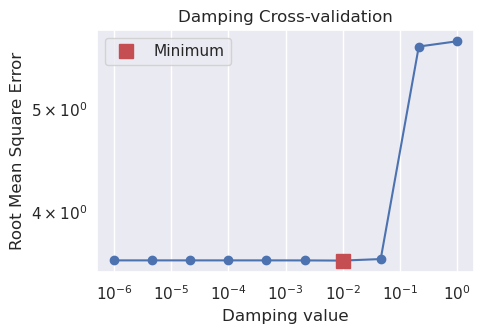
\includegraphics[width=\textwidth]{figures/chp4/RIS_damping_CV.png}
        \caption{}
    \end{subfigure}
    \begin{subfigure}[t]{.4\textwidth}
        \centering
        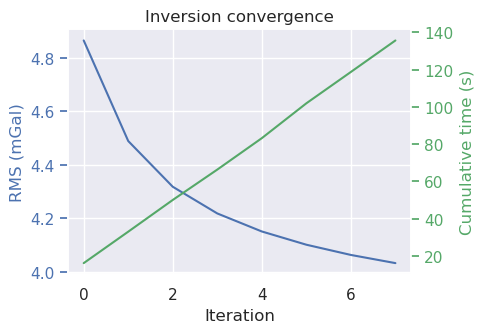
\includegraphics[width=\textwidth]{figures/chp4/RIS_convergence.png}
        \caption{}
    \end{subfigure}
    \begin{subfigure}[t]{.95\textwidth}
        \centering
        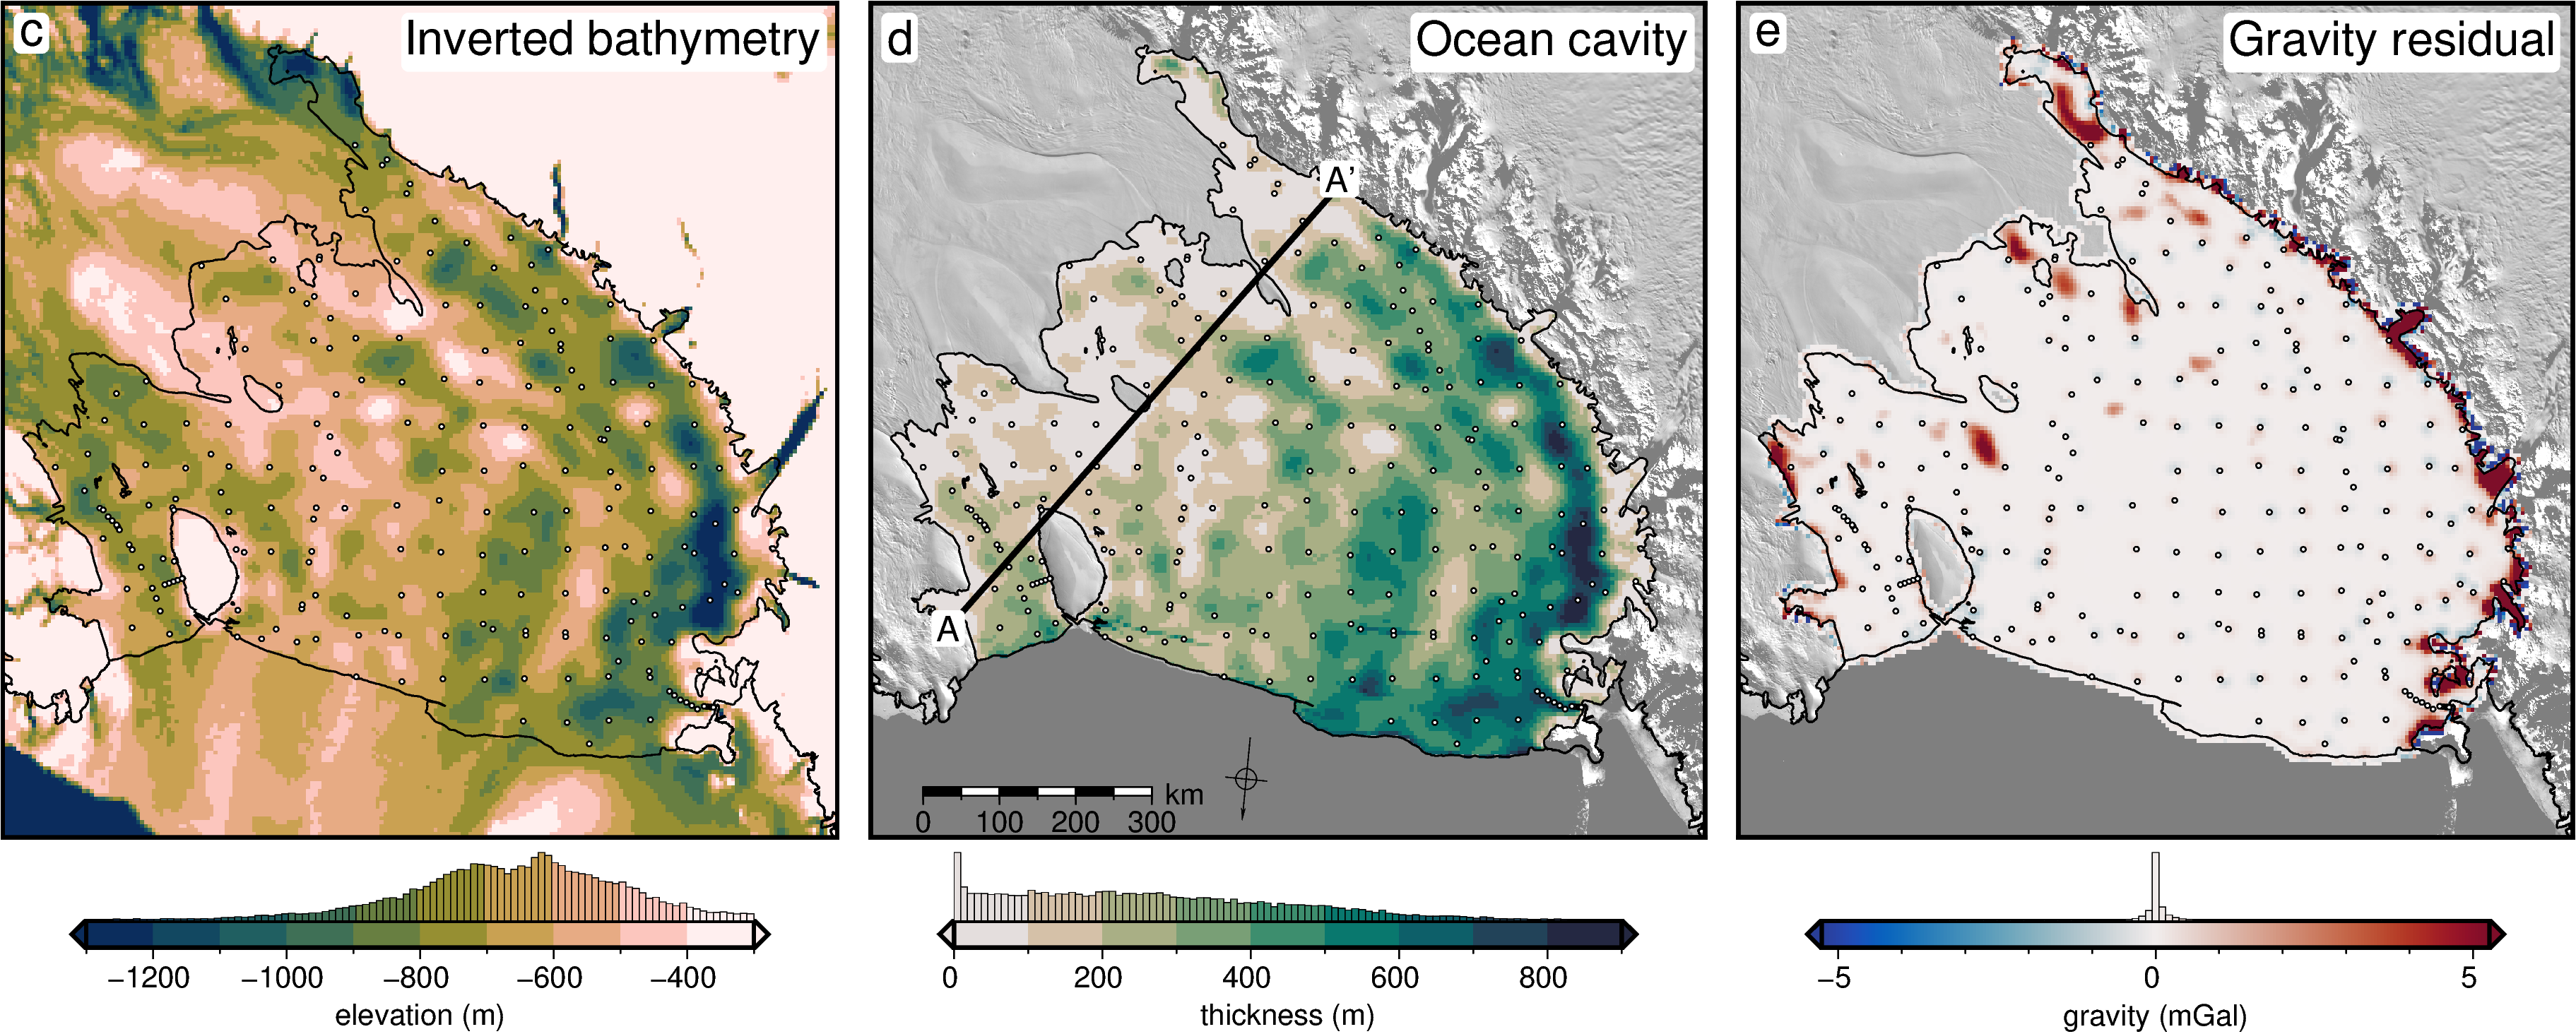
\includegraphics[width=\textwidth]{figures/chp4/RIS_inversion_results.png}
        % \caption{}
    \end{subfigure}
    \begin{subfigure}[t]{.8\textwidth}
        \addtocounter{subfigure}{3}
        \centering
        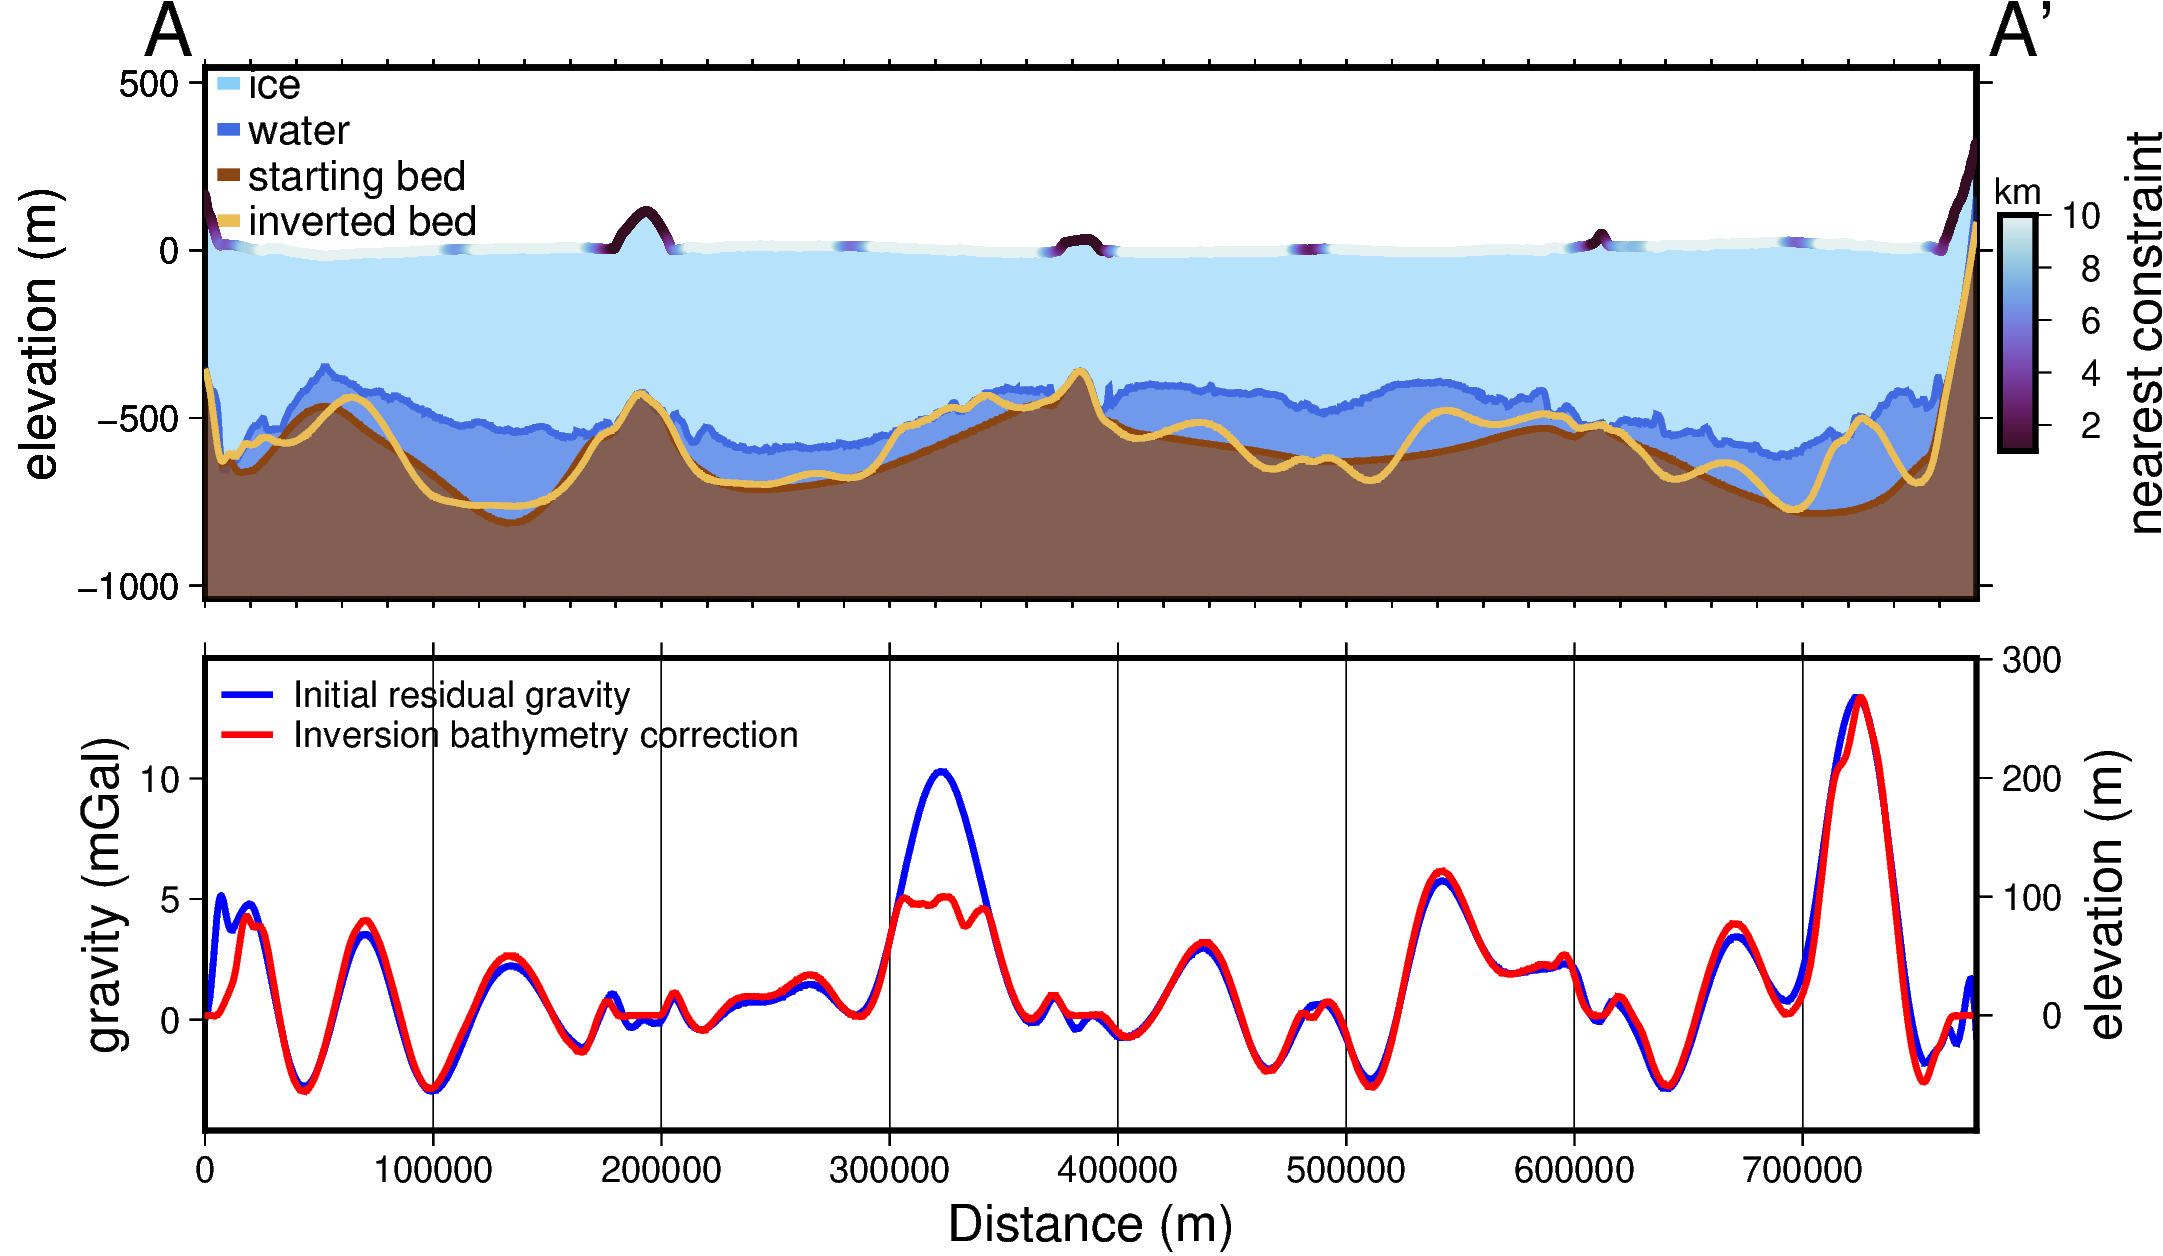
\includegraphics[width=\textwidth]{figures/chp4/RIS_inversion_results_profile.png}
        \caption{}
    \end{subfigure}
  \caption[Ross Ice Shelf singular bathymetry inversion results]{Ross Ice Shelf singular bathymetry inversion results. \textbf{a)} Damping parameter cross-validation with the lowest score shown in red. \textbf{b)} Convergence curve and cumulative inversion time for the optimal inversion. Blue line (left y-axis) shows consecutive iteration's RMS residual component of the topo-free gravity disturbance. Green line (right y-axis) shows cumulative time to run the inversion. \textbf{c)} Inverted bathymetry, \textbf{d)} water column thickness between the inverted bathymetry and Bedmachine v3 icebase \citep{morlighemdeep2020, morlighemmeasures2022}, \textbf{e)} final residual component of the topo-free gravity disturbance. \textbf{f)} \textbf{Profile A to A'}. \textbf{Upper panel} shows ice surface and icebase from BedMachine v3, both the starting bathymetry (dark brown) and the inverted bathymetry (light brown). The colour of the ice surface shows the distance to the nearest constraint point. \textbf{Lower panel} shows the initial residual gravity used as input to the inversion (blue line, left y-axis), and the total correction (red line, right y-axis) applied to the starting bathymetry surface during the inversion to get the inverted bathymetry.}
    \label{fig:chp4_RIS_inversion_results}
\end{figure}

The inverted bathymetry model for the sub-Ross Ice Shelf, at a 5~km resolution, is shown in Figure \ref{fig:chp4_RIS_inversion_results}c. Note that this is just the result of a single inversion. Our final inverted bathymetry model is achieved through the Monte Carlo simulation, as described below. The RMS difference between the inversion results and the starting model at the constraints is 16 m. The thickness of the water column, defined as the difference between BedMachine v3 ice base and the inverted bathymetry, is shown in Figure \ref{fig:chp4_RIS_inversion_results}d. \\

\subsection{Uncertainty}

We used a series of Monte Carlo simulations (Figure \ref{fig:chp4_Monte_Carlo_workflow}) to assess both the spatial uncertainty of the resulting inverted bathymetry and the importance of the various components and parameters of the inversion. By varying the inputs of the inversion within their ranges of uncertainties, we can gather a range of the possible bathymetry results, which when compared shows where the inversion results are more or less certain. The inputs and their respective uncertainty distributions included in the sampling are:
\begin{enumerate}
    \item 
    Gravity disturbance data; sampled from a normal distribution with a mean of the data point, and a standard deviation of the RMS mis-tie of the line data after levelling (3.3~mGal).
    \item 
    Constraint point depths; sampled from a normal distribution with a mean of the measured depth, and a standard deviation of 10~m for points outside of the ice shelf, and 5\% of depth from the ice surface for points within the ice shelf (mean of 36~m).
    \item 
    The density of ice, water, and sediment; all sampled from normal distributions with means of 915~kg~m\textsuperscript{-3}, 1024~kg~m\textsuperscript{-3}, and 2300~kg~m\textsuperscript{-3} respectively, and standard deviations of 5~kg~m\textsuperscript{-3}, 5~kg~m\textsuperscript{-3}, and 400~kg~m\textsuperscript{-3}. The small standard deviations of ice and water compared to sediment reflects the relative certainty of the value and spatial heterogeneity of the density of ice and water, compared to those of the material comprising the sea floor. For the Ross Ice Shelf, the entire region is likely to be draped is at least 10's of meters of sediment \citep[Chapter \ref{ch:2},][]{tankersleybasement2022}. With a mean of 2300~kg~m\textsuperscript{-3} and a standard deviation of 400~kg~m\textsuperscript{-3}, these values span the range from unconsolidated sediment to low-density crystalline rock \citep{schöndensity2015}. 
    \item 
    The tension factor used in minimum curvature gridding for interpolating both the starting bathymetry model and the regional component of gravity. The tension factor values were sampled from a uniform distribution between 0 and 1. 
\end{enumerate}


\begin{figure}[!ht]
  \centering
    \begin{subfigure}[t]{.98\textwidth}
        % \centering
        \hspace*{-1.5cm} %
        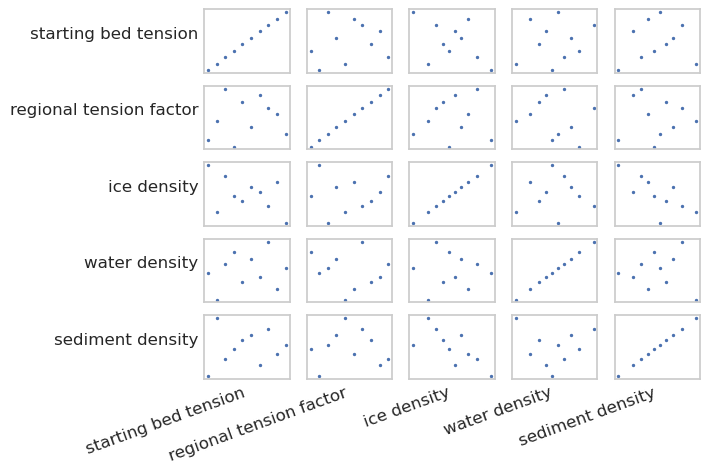
\includegraphics[width=\textwidth]{figures/chp4/RIS_LHC_covariance.png}
        \caption{}
    \end{subfigure}
    \begin{subfigure}[t]{.9\textwidth}
        \centering
        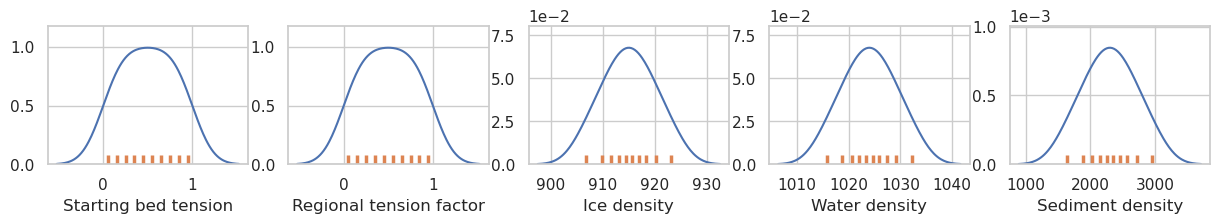
\includegraphics[width=\textwidth]{figures/chp4/RIS_LHC_distributions.png}
        \caption{}
    \end{subfigure}
  \caption[Latin hypercube sampling distributions and correlations]{Latin hypercube sampling results for the 10 inversions of the full Monte Carlo simulation. \textbf{a)} Correlations between each pair of the 5 sampled input parameters. \textbf{b)} Resulting distributions of the 10 sampled values of each parameter. Blue line shows kernel density estimates fit to each set of sampled values, which are shown as orange ticks.}
    \label{fig:chp4_RIS_sampling_results}
\end{figure}

Figure \ref{fig:chp4_RIS_sampling_results} shows the results of the Latin hypercube sampling of the 5 input variables (not including the gravity and constraints data). The correlations between each set of variables show that pairwise correlation was minimal. This is ideal since these inputs are unrelated, and therefore their sampled values should be uncorrelated \citep{heltonsurvey2006}. This also shows that with only 10 samplings, the Latin hypercube sampling was able to provide adequate spatial coverage of the individual distributions (\ref{fig:chp4_RIS_sampling_results}b) as well as all the pairwise distributions combinations (\ref{fig:chp4_RIS_sampling_results}a).

\begin{figure}[!ht]
    \centering
    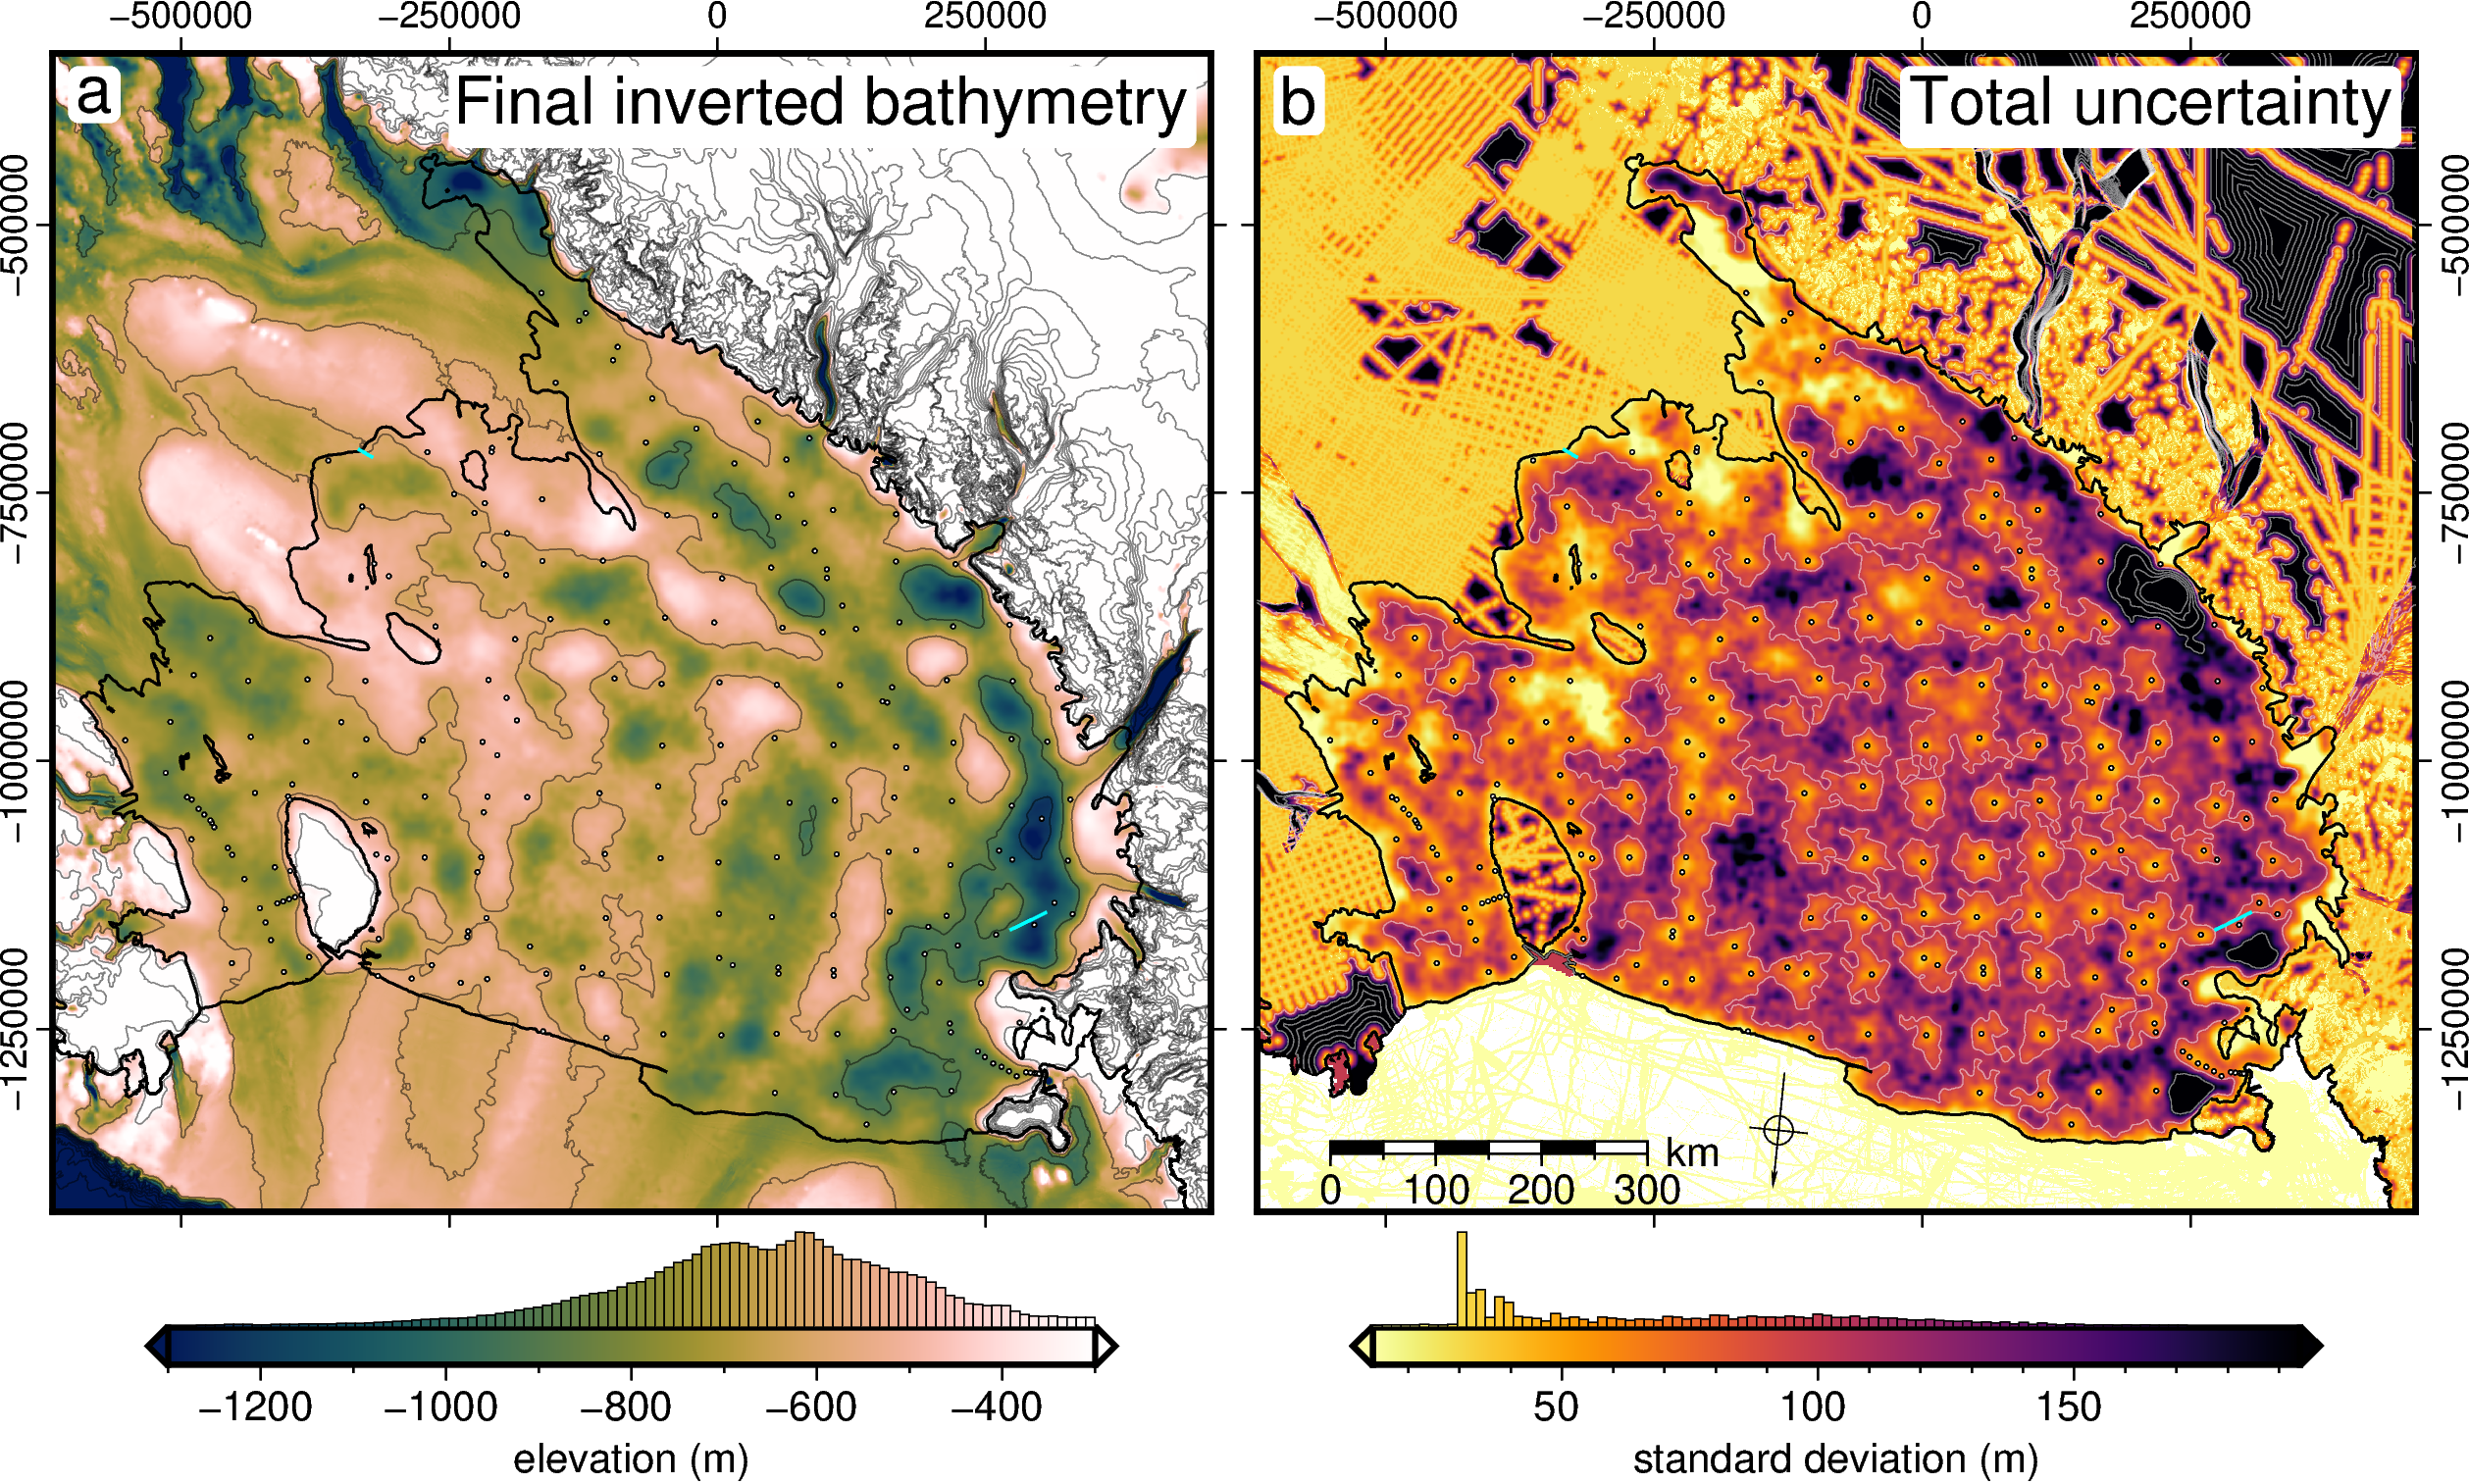
\includegraphics[width=.99\textwidth]{figures/chp4/RIS_MC_bed_and_uncert.png}
    \caption[Ross Ice Shelf inverted bathymetry and uncertainty]{Final bathymetry depths and uncertainties from the full Monte Carlo simulation, merged with 500m resolution elevation and uncertainty data outside of the shelf from BedMachine v3 \citep{morlighemdeep2020, morlighemmeasures2022}. \textbf{a)} Final inverted bathymetry model, calculated as the weighted mean of the full Monte Carlo simulation. Shown with 300~m contours. \textbf{b)} Uncertainty estimation of the inverted bathymetry from the cell-specific weighted standard deviation of the inverted bathymetry results from the full Monte Carlo simulation. Shown with 100~m contours. Constraints within the ice shelf are shown as dots in \textbf{a}. Grounding line and coastline are shown in black \citep{morlighemmeasures2022}. Background imagery is from \citet{scambosmodisbased2007}. Cyan lines show Discovery Deep and Kamb Ice Stream seismic surveys.}
    \label{fig:chp4_RIS_MC_results}
\end{figure}

Each simulation consisted of 10 runs. We performed a \textit{full} simulation, where each of the above inputs were sampled (Figure \ref{fig:chp4_RIS_MC_results}). We performed five additional simulations (Figure \ref{fig:chp4_RIS_MC_sensitivity}) where 1) only the gravity data were sampled, 2) only the constraint point depths were sampled, 3) only the density values of ice, water, and sediment were sampled, 4) only the tension factor for interpolating the starting bathymetry model was sampled, and finally 5) only the tension factor for interpolating the regional component of gravity was sampled. Each simulation results in a series of inverted bathymetries. Finding the cell-specific weighted standard deviation of the bathymetry depths for each of these simulations gives an estimation of the uncertainty resulting from the associated parameter. The cell-specific statistics of these simulations were low-pass filtered to remove high-frequency noise induced by the random sampling. For the full simulation (Figure \ref{fig:chp4_RIS_MC_results}b) the weighted mean of the resulting bathymetries gives the final inverted bathymetry results of this study (Figure \ref{fig:chp4_RIS_MC_results}a). Note that this final bathymetry model resulting from the Monte Carlo simulation is similar, but distinct from the inverted bathymetry resulting from a single inversion without the Monte Carlo simulation, shown in Figure \ref{fig:chp4_RIS_inversion_results}c. \\

\begin{figure}[!ht]
    \centering
    \includegraphics[width=.98\textwidth]{figures/chp4/RIS_MC_sensitivities.png}
    \caption[Monte Carlo results]{Sensitivity analysis for the inversion input data and parameters. Cell-specific weighted standard deviations of the inverted bathymetry results from Monte Carlo simulations with sampling the uncertainties of the \textbf{a)} gravity data, \textbf{b)} constraint points depths, \textbf{c)} ice, water, and sediment density values, \textbf{d)} starting bed interpolation tension factor, and \textbf{e)} tension factor for interpolating the regional gravity component. \textbf{f)} The total uncertainty from the full simulation. 100~m contours in white. Constraints within the ice shelf are shown as dots in \textbf{c}. Grounding line and coastline shown in black \citep{morlighemmeasures2022}. Background imagery is from \citet{scambosmodisbased2007}.}
    \label{fig:chp4_RIS_MC_sensitivity}
\end{figure}

The final bathymetry and uncertainty grids were resampled to a resolution of 500~m, from their original 5~km resolutions, masked outside of the ice shelf, and merged to the 500~m resolution bed and uncertainty data of BedMachine v3. This final bathymetry has a mean elevation of $\sim$-700~m within the ice shelf. The deepest point is $\sim-1370\pm187$~m, located near the Byrd Glacier outlet (Figure \ref{fig:chp4_inversion_inputs}b). Bathymetric features appear to have continuity with features from BedMachine v3 data outside of the ice shelf. The RMS difference between the bathymetry and the original constraint point depths is 44~m. Subtracting the bathymetry from the ice base elevations of BedMachine v3 \citep{morlighemdeep2020, morlighemmeasures2022} gives the water column thickness, as shown in Figure \ref{fig:chp4_RIS_inversion_profiles}b. Without ice base uncertainty estimates from BedMachine v3, we use the bathymetry uncertainty as our uncertainty for the water column thickness, acknowledging that this is a minimum uncertainty. Within the ice shelf boundary, this water column thickness has a mean value of 260~m and a maximum of 1000~m, located near the Nimrod Glacier outlet. Here, the bathymetry has an uncertainty of $\pm$800~m. Outside of this region, the thickest ocean cavity is $\sim940\pm180$~m, located at the Byrd Glacier outlet. The similarity between the bathymetry depth and the water column thickness shows that the ocean cavity is predominantly controlled by bathymetry and that the ice base topography is smooth compared to the bed. The uncertainty in the bed elevation ranges from $\sim$10~-~850~m, with a mean of 95~m (Figure \ref{fig:chp4_RIS_inversion_results}b). It has an approximately normal distribution, with a slight skew to the higher values. In general, the uncertainty is lowest at the constraint points and highest far from constraints. There are elevated uncertainties in several spots, with the largest being along the Transantarctic mountain front.\\

\subsubsection{Partitioning uncertainty}

The uncertainty in the inverted bathymetry which arises from the uncertainty in gravity data (Figure \ref{fig:chp4_RIS_MC_sensitivity}a) is relatively spatially uniform, with a mean of 85~m. It is lowest immediately at the constraint points, and generally highest far from constraint points. The uncertainty from the constraint point depths (Figure \ref{fig:chp4_RIS_MC_sensitivity}b) is also generally spatially uniform, with a mean of 10~m. Conversely, it is highest at the constraint points, and lowest far from constraint points. The uncertainty resulting from the choice of density values (Figure \ref{fig:chp4_RIS_MC_sensitivity}c) displays a more heterogeneous spatial distribution than the previous two uncertainties. It is lowest at the constraint points and has a mean of 24~m. The largest values are located at the gaps between constraint points. The uncertainty resulting from the interpolation of the starting bed (Figure \ref{fig:chp4_RIS_MC_sensitivity}d) has a distinct spatial distribution. It is highest along the Transantarctic Mountain front, with values up to 40~m, but it has an overall mean of 7~m. Lastly, the uncertainty resulting from the estimation and removal of the regional component of gravity, prior to the inversion, (Figure \ref{fig:chp4_RIS_MC_sensitivity}e), also shows highest values along the mountain front, with values over 200~m (up to 700~m at the Nimrod Glacier outlet). The mean value is 24~m. The reported uncertainties and their components from a wide range of past studies are shown in Table \ref{table:chp4_past_study_uncertainties}. \\


\begin{table}
\footnotesize 
\centering
\begin{tblr}{
  width = \linewidth,
  colspec = {Q[350]Q[140]Q[155]Q[160]Q[195]},
  cell{1}{2} = {c=4}{0.597\linewidth,c},
  vline{2} = {3-24}{},
  hline{2} = {2-5}{},
  hline{3} = {-}{},
  hline{25} = {-}{},
}
                                  & Inverted bathymetry uncertainty (m) & & &                 \\
Study                             & total  & from gravity  & from geology  & from constraints \\
\textbf{This study} ($\overline{x}\pm1\sigma$) & 95$\pm$51 & 85$\pm$32     & 48$\pm$30    & 10$\pm$6 \\
\citet{eisermannbathymetric2021}   & 220               & 84          & 116        & 20     \\
\citet{tintobathymetry2015}        & 160               & 26          & 124        & 10     \\
\citet{constantinoseafloor2020}    & 133               & 34          & 90         & 5-10   \\
\citet{boghosianresolving2015}     & 110               & 10-28       & 50-70      & 10     \\
\citet{tintoprogressive2011}       & 70                & 34          & 10-15      & 20     \\
\citet{constantinocook2023}        & 69-123            & 32-39       & 27-74      & 10     \\
\citet{tintoross2019}              & 68                & 48          & 10         & 10     \\
\citet{eisermannbathymetry2020}    & 175-225           & -           & -          & 10     \\
\citet{jordannew2020}              & 100               & 23          & -          & -      \\
\citet{anbathymetry2019}           & 60                & 60          & -          & -      \\
\citet{studingerestimating2004}    & 250               & -           & -          & -      \\
\citet{weigetz2020}                & 246               & -           & -          & -      \\
\citet{greenbaumocean2015}         & 190               & -           & -          & -      \\
\citet{brisbourneseabed2014}       & 160               & -           & -          & -      \\
\citet{hodgsonfuture2019}          & 100               & -           & -          & -      \\
\citet{yangbathymetry2021}         & 68                & -           & -          & -      \\
\citet{anbed2017}                  & 60                & -           & -          & -      \\
\citet{millanbathymetry2017}       & 50-65             & -           & -          & -      \\
\citet{millanvulnerability2018}    & 30-50             & -           & -          & -      \\
\citet{millanconstraining2020}     & 45                & -           & -          & -      \\
\citet{filinanew2008}              & -                 & 19          & -          & -      \\
\textbf{Mean}                      & 117 (N=25)        & 40 (N=13)   & 57 (N=11)  & 12 (N=10)
\end{tblr} 
\caption[Bathymetry uncertainties comparison]{Reported inverted bathymetry uncertainties and the various components. Our reported geologic uncertainty is the combination of uncertainties resulting from the density values and the tension factor used in grinding the regional field.}
\label{table:chp4_past_study_uncertainties}
\end{table}

% \citet{constantinoseafloor2020} total of 133 m,  34m from 2.4mgal cross over using bouguer slab, 5-10 from constraints, and 90 from density variations,
% \citet{eisermannbathymetry2020} totals of 175m, 225m, and 210m,
% 10m from ice thickness uncertainty, rest from gravity and density assumptions
% \citet{tintoross2019} 68m total, 48m for 3.2mGal bouguer slab, 10m from constraints, and 3\% (10m) from density
% \citet{jordannew2020} total of 100 m, 23 m from 1.56 mGal crossover and 130 m uncert if using 2500 instead of 2670, 
% \citet{yangbathymetry2021} 68 m 
% \citet{millanconstraining2020} 45 m, 
% \citet{boghosianresolving2015} 110 m, 10-28 m from gravity data, 10m from constraints, 50-70m from density,
% \citet{hodgsonfuture2019} 100 m,
% \citep{anbathymetry2019} 60 m, from 5mGal/100m of water
% \citet{tintobathymetry2015} 160 m total, 124 m from geologic variations, 26m from gravity data, 10 from constraints
% \citet{greenbaumocean2015} 190m total from comparison of grounded ice base from radar and inverted bed 
% \citep{brisbourneseabed2014} 160 m from RMS with constraints
% \citep{weigetz2020} 246 m from comparison of grounded ice base from radar and inverted bed 
% wavelengths resolved by the gravity system, 


\section{Discussion}

Here we discuss the results of our Ross Ice Shelf bathymetry model from the inversion of airborne gravity data. First, we describe the results of the uncertainty and parameter sensitivity analysis. Then we compare our results with two past bathymetry models beneath the Ross Ice Shelf and discuss the differences. Lastly, we discuss various implications of this updated bathymetry model, including how the findings relate to geology, tectonics, and ice sheet dynamics. %Lastly, we suggest future work with aims to improve our understanding of the sub-Ross Ice Shelf bathymetry. 

\subsection{Uncertainties and parameter importance}

The results of our Monte Carlo simulations provide answers to several important questions. 1) Wow confident are we in the inverted bathymetry depths? 2) Where are we most and least confident about the bathymetry depth? 3) What are the specific sources of this uncertainty? and finally, 4) What can be done to limit the uncertainty? Figures \ref{fig:chp4_RIS_MC_results}b and \ref{fig:chp4_RIS_MC_sensitivity}f show the resulting spatial uncertainty of the inverted bathymetry, providing an answer to the first two questions. To determine the sources of this uncertainty, the individual inputs to the inversion were isolated and their effects on the estimated uncertainty were found (Figure \ref{fig:chp4_RIS_MC_sensitivity}).\\

\subsubsection{Gravity component}
 The largest contributor to the overall uncertainty of the inversion is the uncertainty of the gravity data (Figure \ref{fig:chp4_RIS_MC_sensitivity}a). This uncertainty resulting from the gravity data results in a base-level bathymetry uncertainty of $\sim$~85~m and is relatively spatially uniform. This is because each gridded gravity data point is contaminated with independent noise of varying levels during the Monte Carlo sampling. It is this point-by-point random noise that creates the noisy component in the final inverted bathymetry. In reality, the uncertainty of nearby gravity data is likely correlated, where entire lines, or sections of lines have similar uncertainty values, due to changing data collection conditions, like turbulence, or mis-levelling, causing values of entire lines to be offset, or tilted. Here our estimate of gravity uncertainty is entirely dependent on cross-over misties; likely an oversimplified estimation of uncertainty for an entire survey. This suggests that the true uncertainty resulting from the gravity data likely has a different spatial distribution and may be larger than we report; a finding which is not surprising, since the entire method depends on these data.\\ 

\subsubsection{Constraints component}
 The uncertainty in the other data input to the inversion, the constraint point depths, has only a small effect on the results (Figure \ref{fig:chp4_RIS_MC_sensitivity}b). It is worth noting that while the uncertainty resulting from the constraint point measurement uncertainty is low, the constraints themselves are fundamental to the inversion. These constraints feed into all the components of the inversion and thus affect the uncertainty of each component, including the uncertainty from the gravity data. This is shown by the correlation between uncertainty and the distance to the nearest constraint (Figure \ref{fig:chp4_RIS_weighting_grid}) of all the components of Figure \ref{fig:chp4_RIS_MC_sensitivity}. Our Monte Carlo sensitivity analysis only tests the effects of estimated noise in the inputs, and not their overall importance for the inversion. Since the uncertainty in the constraints only impacts the inversion in the immediate vicinity of the constraint, for constraint data collection, efforts should be focused on quantity over quality, assuming the uncertainty can be limited to a reasonable amount. In practice, for over-ice seismic surveying, this may lead to the choice of fast and efficient systems as opposed to high-resolution systems, if the main goal of the survey is to collect bathymetry constraints. For example, towable snow streamers and sources such as surface detonations or vibroseis \citep[e.g.,][]{hofstedeevidence2021, smithdetailed2020} can collect data very efficiently ($\sim20$~km/day), compared to higher-resolution surveys with buried geophone arrays and drill-emplaced explosives \citep[e.g.,][]{horgansediment2013}. The remaining sources of uncertainty are related to user-defined inversion parameters.\\

\subsubsection{Density component}
The choice of density values for the ice, water, and sediment results in a mean uncertainty in the bathymetry model of 24~m (Figure \ref{fig:chp4_RIS_MC_sensitivity}c). The ranges of densities tested in the Monte Carlo simulation were $\sim$ 905~-~925~kg~m\textsuperscript{-3} for ice\footnote{We note that the maximum density of meteoric ice is 917~kg~m\textsuperscript{-3}, however; the inclusion of marine ice may raise this value \citep{frickerdistribution2001}}, $\sim$ 1015~-~1035~kg~m\textsuperscript{-3} for seawater, and $\sim$~1600~-~3000~kg~m\textsuperscript{-3} for the seafloor. We only test homogeneous changes in the density values.\\

The uncertainty arising from the choice in density values has a strong spatial correlation with the absolute value of the inversion's input gravity, the residual gravity (Figure \ref{fig:chp4_RIS_terrain_regional_residual}d). This correlation can be explained by the inverse relation between the amplitude of the corrections applied to the bathymetry during the inversion, and the density contrasts used in the inversion. For the same gravity anomaly, a smaller density contrast results in a larger amplitude correction while a larger density contrast results in a smaller correction. This means that changes in the density values just affect the amplitude of the correction applied to the bathymetry. Often, spatially variable density is used as a means to account for the regional component of gravity \citep[e.g.,][]{tintoross2019, constantinoseafloor2020}. We note that there is an additional benefit to incorporating spatially variable densities. If adequate \textit{a priori} information is known to justify a density distribution, this can be used to allow differing amplitudes of corrections across the inversion domain. In other words, if the seafloor truly is denser in one region of the inversion compared to the seafloor elsewhere, for a similar gravity anomaly, the inversion correction should be of smaller amplitude in the high-density region. However, due to a lack of geologic knowledge beneath the ice shelf, we use constant density values. We propose Monte Carlo sampling of a wide range of possible density values as a robust and feasible method to avoid biasing the resulting bathymetry model to either too high or too low correction amplitudes, to achieve both the most realistic results and an estimation of the uncertainty.\\

\subsubsection{Interpolation component}
The final components of the overall uncertainty are related to interpolation conducted during two stages of the inversion; 1) the interpolation of the starting model from the sparse constraint point depths, and 2) the estimation of the regional field from the interpolation of gravity values at the constraint points. Here, we have used a minimum curvature gridding algorithm \citep{smithgridding1990}, which accepts a tension factor for the interpolation which can range from 0 to 1. Figure \ref{fig:chp4_starting_bed_comparison} shows the results of six different values of this tension factor for creating the starting bed model. These figures show that low values of tension are able to accurately reproduce the data with a smooth interpolation, but can result in unconstrained local maxima or minima. Conversely, high tension values produce smooth surfaces without false oscillations but don't adhere to the data as well. For these issues associated with the two end members, intermediate values of 0.25 and 0.35 are often suggested for potential field data and topographic data, respectively. We suggest a more robust alternative to using these suggested values is the Monte Carlo sampling approach we have used. This runs the inversion with a variety of tension factors and uses the standard deviation of the resulting bathymetry models as a means to estimate the uncertainty associated with the choice of the tension factor. While tensioned minimum curvature gridding has been used in several past inversions \citep[e.g.,][]{yangbathymetry2021, millanconstraining2020, anbathymetry2019}, the choice of the tension values has not been discussed for these applications. \\ 

The uncertainties arising from the choice of tension factors are shown in Figure \ref{fig:chp4_RIS_MC_sensitivity}d and e. The tension factor for gridding the starting bed model results in a relatively low uncertainty with a mean of 7~m. The resulting uncertainty for the regional separation is comparatively high, with a mean of 24~m. Both of these results show large spatial heterogeneity, with significantly larger uncertainties along the Transantarctic Mountain front. This is likely related to the poor performance of this gridding algorithm for high-gradient data. This region along the mountain front has both steep topography and high amplitude gravity anomalies. \\

\subsubsection{Reducing uncertainties}

Of the various components of the uncertainty analysis, only some can feasibly be reduced. Reducing the uncertainty resulting from the interpolation parameters may be possible with future method development, but this is beyond the discussion of this research. To our knowledge, there is no robust method of determining a spatially variable density distribution to be used in the inversion, without the collection of in-situ data. This leaves the data inputs, gravity and constraints, as viable components of a bathymetry inversion where further reductions of uncertainties can occur. We propose a favourability of quantity over quality for constraint data since typical bed elevation uncertainty is already relatively low, and therefore more data of mediocre quality should be prioritized over high-quality but spatially limited data. In order to reduce the uncertainty component resulting from the gravity data, first we must be able to estimate the realistic spatial uncertainty of the gravity data itself. A simple cross-over analysis is too simple to cover the effects of turbulence, changing flight speed and altitude, and errors in processing steps, such as base station ties and levelling. The areas of largest uncertainty are generally a function of 1) distance to the nearest constraint point (Figure \ref{fig:chp4_RIS_weighting_grid}) and 2) proximity to steep gradients of topography and/or gravity (Figure \ref{fig:chp4_RIS_MC_sensitivity}d and e). This highlights the entire Transantarctic Mountain front of the Ross Ice Shelf and the two major constraint gaps in the central-east portion of the ice shelf (Figure \ref{fig:chp4_RIS_weighting_grid}) as locations that would greatly benefit from additional seismic surveying. 

\subsubsection{Past estimations of uncertainty}

Our comprehensive uncertainty and sensitivity analysis is shown to be similar to the approximated uncertainties reported for other ice shelves (Table \ref{table:chp4_past_study_uncertainties}). Some differences include; our reported uncertainty resulting from the gravity data uncertainty is the highest reported, while our values resulting from other sources, and the total uncertainty, were similar to those of other studies. Our larger reported uncertainty resulting from the gravity data likely shows that the simple Bouguer slab approximation used by the other studies underestimates the component of uncertainty resulting from the gravity data uncertainty. We take the uncertainties resulting from geologic variations to be the combination of our reported uncertainties from the chosen density values (Figure \ref{fig:chp4_RIS_MC_sensitivity}c) and from the regional separation gridding (Figure \ref{fig:chp4_RIS_MC_sensitivity}e) since these both affect the estimation of the regional component. The uncertainty resulting from the constraint point measurement uncertainty was very similar across all studies.\\

From this, we propose future bathymetry inversions undertake similar uncertainty analysis through the Monte Carlo sampling of the input parameters. This technique not only provides similar uncertainty estimates to past studies, but it accomplishes it in a systematic and reproducible method. Additionally, this technique provides a spatial distribution of the uncertainties, instead of a single value. Once the inversion workflow is set up, the sampling and re-running of the inversion is a simple procedure, and with the use of Latin hypercube sampling, we have shown that with only 10 runs, the parameter space of all the inputs is adequately sampled (Figure \ref{fig:chp4_latin_hypercube_sampling}).\\

\subsection{Past bathymetry models}

Our gravity-inverted bathymetry model for the sub-Ross Ice Shelf reveals significant differences with previous bathymetry models. However, a portion of these differences are not related to the inversion, but to the creation of the starting model. First, we will discuss the differences between our starting bathymetry model and another interpolation-based bathymetry model, then we will compare our inversion results with two past models. These past models include Bedmap2 \citep{fretwellbedmap22013} and Bedmachine v3 \citep{morlighemdeep2020, morlighemmeasures2022}. The Bedmap2 model for the Ross Ice Shelf region is created from the interpolation of the same constraint points within the ice shelf as used in this study, as well as grounded ice thickness measurements and limited rock outcrop elevation data \citep{fretwellbedmap22013, lebrocqimproved2010, timmermannconsistent2010}. BedMachine v3 used these point measurements and applied additional methods to increase the resolution of the bed. For outside of the ice shelf, this included mass conservation for areas of fast-moving ice (outlet glaciers and ice streams), streamline diffusion for regions of slow-moving ice, as well as minimum curvature gridding to interpolate the remaining gaps \citep{morlighemdeep2020}. Within the ice shelf, BedMachine used the gravity inversion results of \citet{tintoross2019}.\\

\subsubsection{Starting model comparison}

Figure \ref{fig:chp4_starting_bed_comparison} shows the series of six starting bed models we created from the interpolation of the sparse constraints. These were created with six levels of tension applied to a minimum curvature interpolation. The cell-specific standard deviation of these six models shows the uncertainty associated with this interpolation (Figure \ref{fig:chp4_starting_bed_comparison}g), and the mean of the six grids is our chosen starting model (Figure \ref{fig:chp4_starting_bed_comparison}h) This is compared with the Bedmap2 model in (Figure \ref{fig:chp4_starting_bed_comparison}i). The RMS difference between the two grids, within the ice shelf, is 95~m. Our starting bed is deeper proximal to the entire grounding zone, while it is shallower along the ice front and throughout the centre of the ice shelf. However, these differences of up to 200~m do not suggest our starting model is inaccurate. Sampling the grid values at the constraint points and comparing them with the constraint depths shows that our model was significantly better at adhering to these constraints, compared to Bedmap2. The RMS of the difference with our model was 14~m, while the RMS of Bedmap2 was 138~m (Figure \ref{fig:chp4_inversion_inputs}).\\

These large differences for Bedmap2 are concentrated along the Transantarctic Mountain front, where the interpolation algorithm used in Bedmap2 resulted in excessively shallow bathymetry. This interpolation appears to have favoured smoothness over accuracy for this location of steep terrain. This has resulted in a "leakage" of the high elevations within the mountains into the bathymetry interpolation, as pointed out in this region \citep{lebrocqimproved2010}, as well as for other ice shelves \citep{brisbourneupdated2020}. This over-smoothing and "leakage", while strongest along the mountain front, can be seen along the entire grounding zone. This is the reason why Bedmap2 was shallower than our starting model along the grounding line. This shows that care needs to be taken when picking or creating a starting model for an inversion, especially in regions of steep topography. The re-creation of the starting model from the point data allows the choice of interpolation techniques better suited for the region of interest, compared to techniques determined most suitable for a continent-wide study.\\

\subsubsection{Inversion result comparisons}

\begin{figure}[!ht]
    \centering
    \includegraphics[width=.98\textwidth]{figures/chp4/RIS_bed_model_comparisons.png}
    \caption[Inverted bathymetry comparisons]{Comparison of our inverted bathymetry with past models. \textbf{a)} Bedmap2 bathymetry, \textbf{b)} our inversion results, from the weighted mean of the full Monte Carlo simulation, and \textbf{c)} BedMachine bathymetry. All three share the same colour scale and are contoured at 400 m intervals. RMS difference with the constraint points for each model is stated on the maps. \textbf{d)} Difference between our model and Bedmap2, \textbf{e)} difference between Bedmap2 and BedMachine v3, and \textbf{f)} difference between our model and BedMachine v3. Grids share a colour scale and are contoured at 100 m intervals. Blue regions in \textbf{d} and \textbf{f} indicate where our results are shallower, while red regions indicate where our results are deeper than the past models. Blue regions in \textbf{e} indicate where BedMachine is shallow, while red regions indicate where BedMachine is deeper than Bedmap2. RMS differences are stated on the maps. Grounding line and coastline are shown in black \citep{morlighemmeasures2022}. Background imagery is from \citet{scambosmodisbased2007}. Elevations are referenced to the WGS-84 ellipsoid.}
    \label{fig:chp4_RIS_bed_model_comparison}
\end{figure}

\paragraph*{Bedmap2 comparison}

Figure \ref{fig:chp4_RIS_bed_model_comparison} compares our final bathymetry results with the models of Bedmap2 and BedMachine v3. Additionally, several profiles across different regions are shown in Figure \ref{fig:chp4_RIS_inversion_profiles}, comparing the various models. Interestingly, the inversion has raised the RMS difference with Bedmap2, compared to the starting model. But due to the issues with the Bedmap2 grid along the mountain front, this increased difference is expected. The differences between our inverted bed and Bedmap2 have a normal distribution (Figure \ref{fig:chp4_RIS_bed_model_comparison}d). Our results introduce many small-scale features, as expected since Bedmap2 is an inherently smooth product. However, there are several noticeable large-scale differences with Bedmap2. Proximal to the grounding line, our results are generally deeper, as seen with the starting model comparison (Figure \ref{fig:chp4_RIS_inversion_profiles}g). Many of the regions where our results are deeper are related to the issue of over-shallow interpolation of Bedmap2. Portions of the grounding zone along the Siple Coast are over 200~m deeper, including the Kamb (Figure \ref{fig:chp4_RIS_inversion_profiles}c) and Mercer ice stream grounding zones. \\

Another notable difference is an NW-SE oriented trough which appears in our results but is essentially absent in Bedmap2. This feature begins at the southern end of the Crary Ice Rise grounding zone and continues $\sim300$~km, paralleling the mountain front (Figure \ref{fig:chp4_RIS_inversion_profiles}c). This feature is the southwestern-most of a series of 2 or 3 parallel troughs and ridges, as shown in Figure \ref{fig:chp4_RIS_inversion_profiles}d. These features are oriented at a high angle to both E-W and N-S flight lines, increasing their likelihood as true features of the bathymetry and not flight line levelling artifacts. While they are subtle, their presence alters the general \textit{texture} in the region from a primary N-S / NNE-SSW to an NW-SW orientation. This switches the general trend of bathymetry features in the region to be aligned with Siple Coast ice flow, rather than the Transantarctic outlet glacier ice flow. Whether these bedforms are tectonic in nature, revealing the tectonic fabric, or are erosion/depositional, and thus revealing the past flow directions of the previously grounded ice sheet is unknown. The last major difference with Bedmap2 is a significantly deeper bathymetry along the western edge of Roosevelt Island (Figure \ref{fig:chp4_RIS_inversion_profiles}a).\\


\paragraph*{Bedmachine comparison}

Comparing our results to Bedmachine v3 provides a unique opportunity to evaluate the differences resulting from different gravity inversion algorithms. The gravity inversion results of \citet{tintoross2019}, which comprise the Bedmachine v3 data beneath the ice shelf, used similar input datasets (gravity data and constraint points), suggesting that differing inversion algorithms and workflows are likely responsible for the majority of the differences shown in Figure \ref{fig:chp4_RIS_bed_model_comparison}f. However, some of the differences may arise from re-processing the gravity data, and a different method of gravity reduction applied here, as compared in Section \ref{chp4:past_inversions}.\\

% Additionally, we have incorporated additional constraint points. These include the Little America Station Byrd Trail seismic survey (1958) between Roosevelt Island and King Edward VII peninsula, the Victoria Land Traverse (1958-59) and the Discovery Deep Traverse (1960), from Roosevelt Island across the ice front to the Skelton Glacier, and the Ross Ice Shelf Traverse (1957-58), a large traverse encompassing most of the ice shelf in a triangle between Roosevelt Island, Minna Bluff, and Crary Ice Rise. See \citet{bennettgravity1964} for descriptions of these traverses.

To remove the regional component of gravity, \citet{tintoross2019} used a smoothly varying density model in their inversion. To create this density model, they created an initial prism layer with prisms extending from their starting bathymetry to a depth of 60~km. With the gravity disturbance, they performed a density inversion to recover the density of each prism. This spatially variable density was then low-pass filtered, with a 50~km cutoff. Incorporating this remaining long-wavelength gravity signal within the density model removed the regional component from the gravity input to the inversion. This technique is conceptually similar to high-pass filtering the gravity data to remove the long-wavelength component. For the inversion, \citet{tintoross2019} used the commercial software Geosoft Oasis Montaj. Limited information is available from Geosoft as to the specifics of this inversion procedure.\\

Comparing our bathymetry (Figure \ref{fig:chp4_RIS_bed_model_comparison}f), there is a normal distribution of differences, centred on zero. The RMS difference between the two grids is $\sim$100~m. Comparing each grid to the constraint point depths, the BedMachine grid has an RMS difference of 92~m, compared to our RMS of 44~m. Generally, our results are approximately 50-100~m deeper proximal to most of the Siple Coast grounding line. Conversely, our results are approximately 50-100~m shallower along the Transantarctic Mountain front. This could be due to our inability to fully fix the issue of overly-shallow interpolation of data along the mountain front in the creation of our starting model, as discussed.\\

Alternatively, the differences could be a result of the different gravity reduction steps. Figure \ref{fig:chp4_RIS_terrain_regional_residual}b and e show that correcting the gravity disturbance for the terrain mass effect results in a large negative topo-free disturbance along the Transantarctic Mountain front (dark blues in \textbf{b}). During the regional field estimation, fitting a spline to these large negative values would bring down the nearby regional field, resulting in an underestimation of the regional (more negative), and thus an overestimation of the residual (positive values). This is shown by the profile of Figure \ref{fig:chp4_RIS_terrain_regional_residual}e. On the right side, along the mountain front, in an attempt to fit the negative values of the topo-free disturbance (red dashed line), the regional field (blue) has been underestimated, leaving a large positive residual anomaly (pink dashed). This positive residual results in a shallowing of the inverted bathymetry.\\

\begin{figure}[p]
% \renewcommand\thesubfigure{\arabic{subfigure}}
  \centering
    \begin{subfigure}[t]{.8\textwidth}
        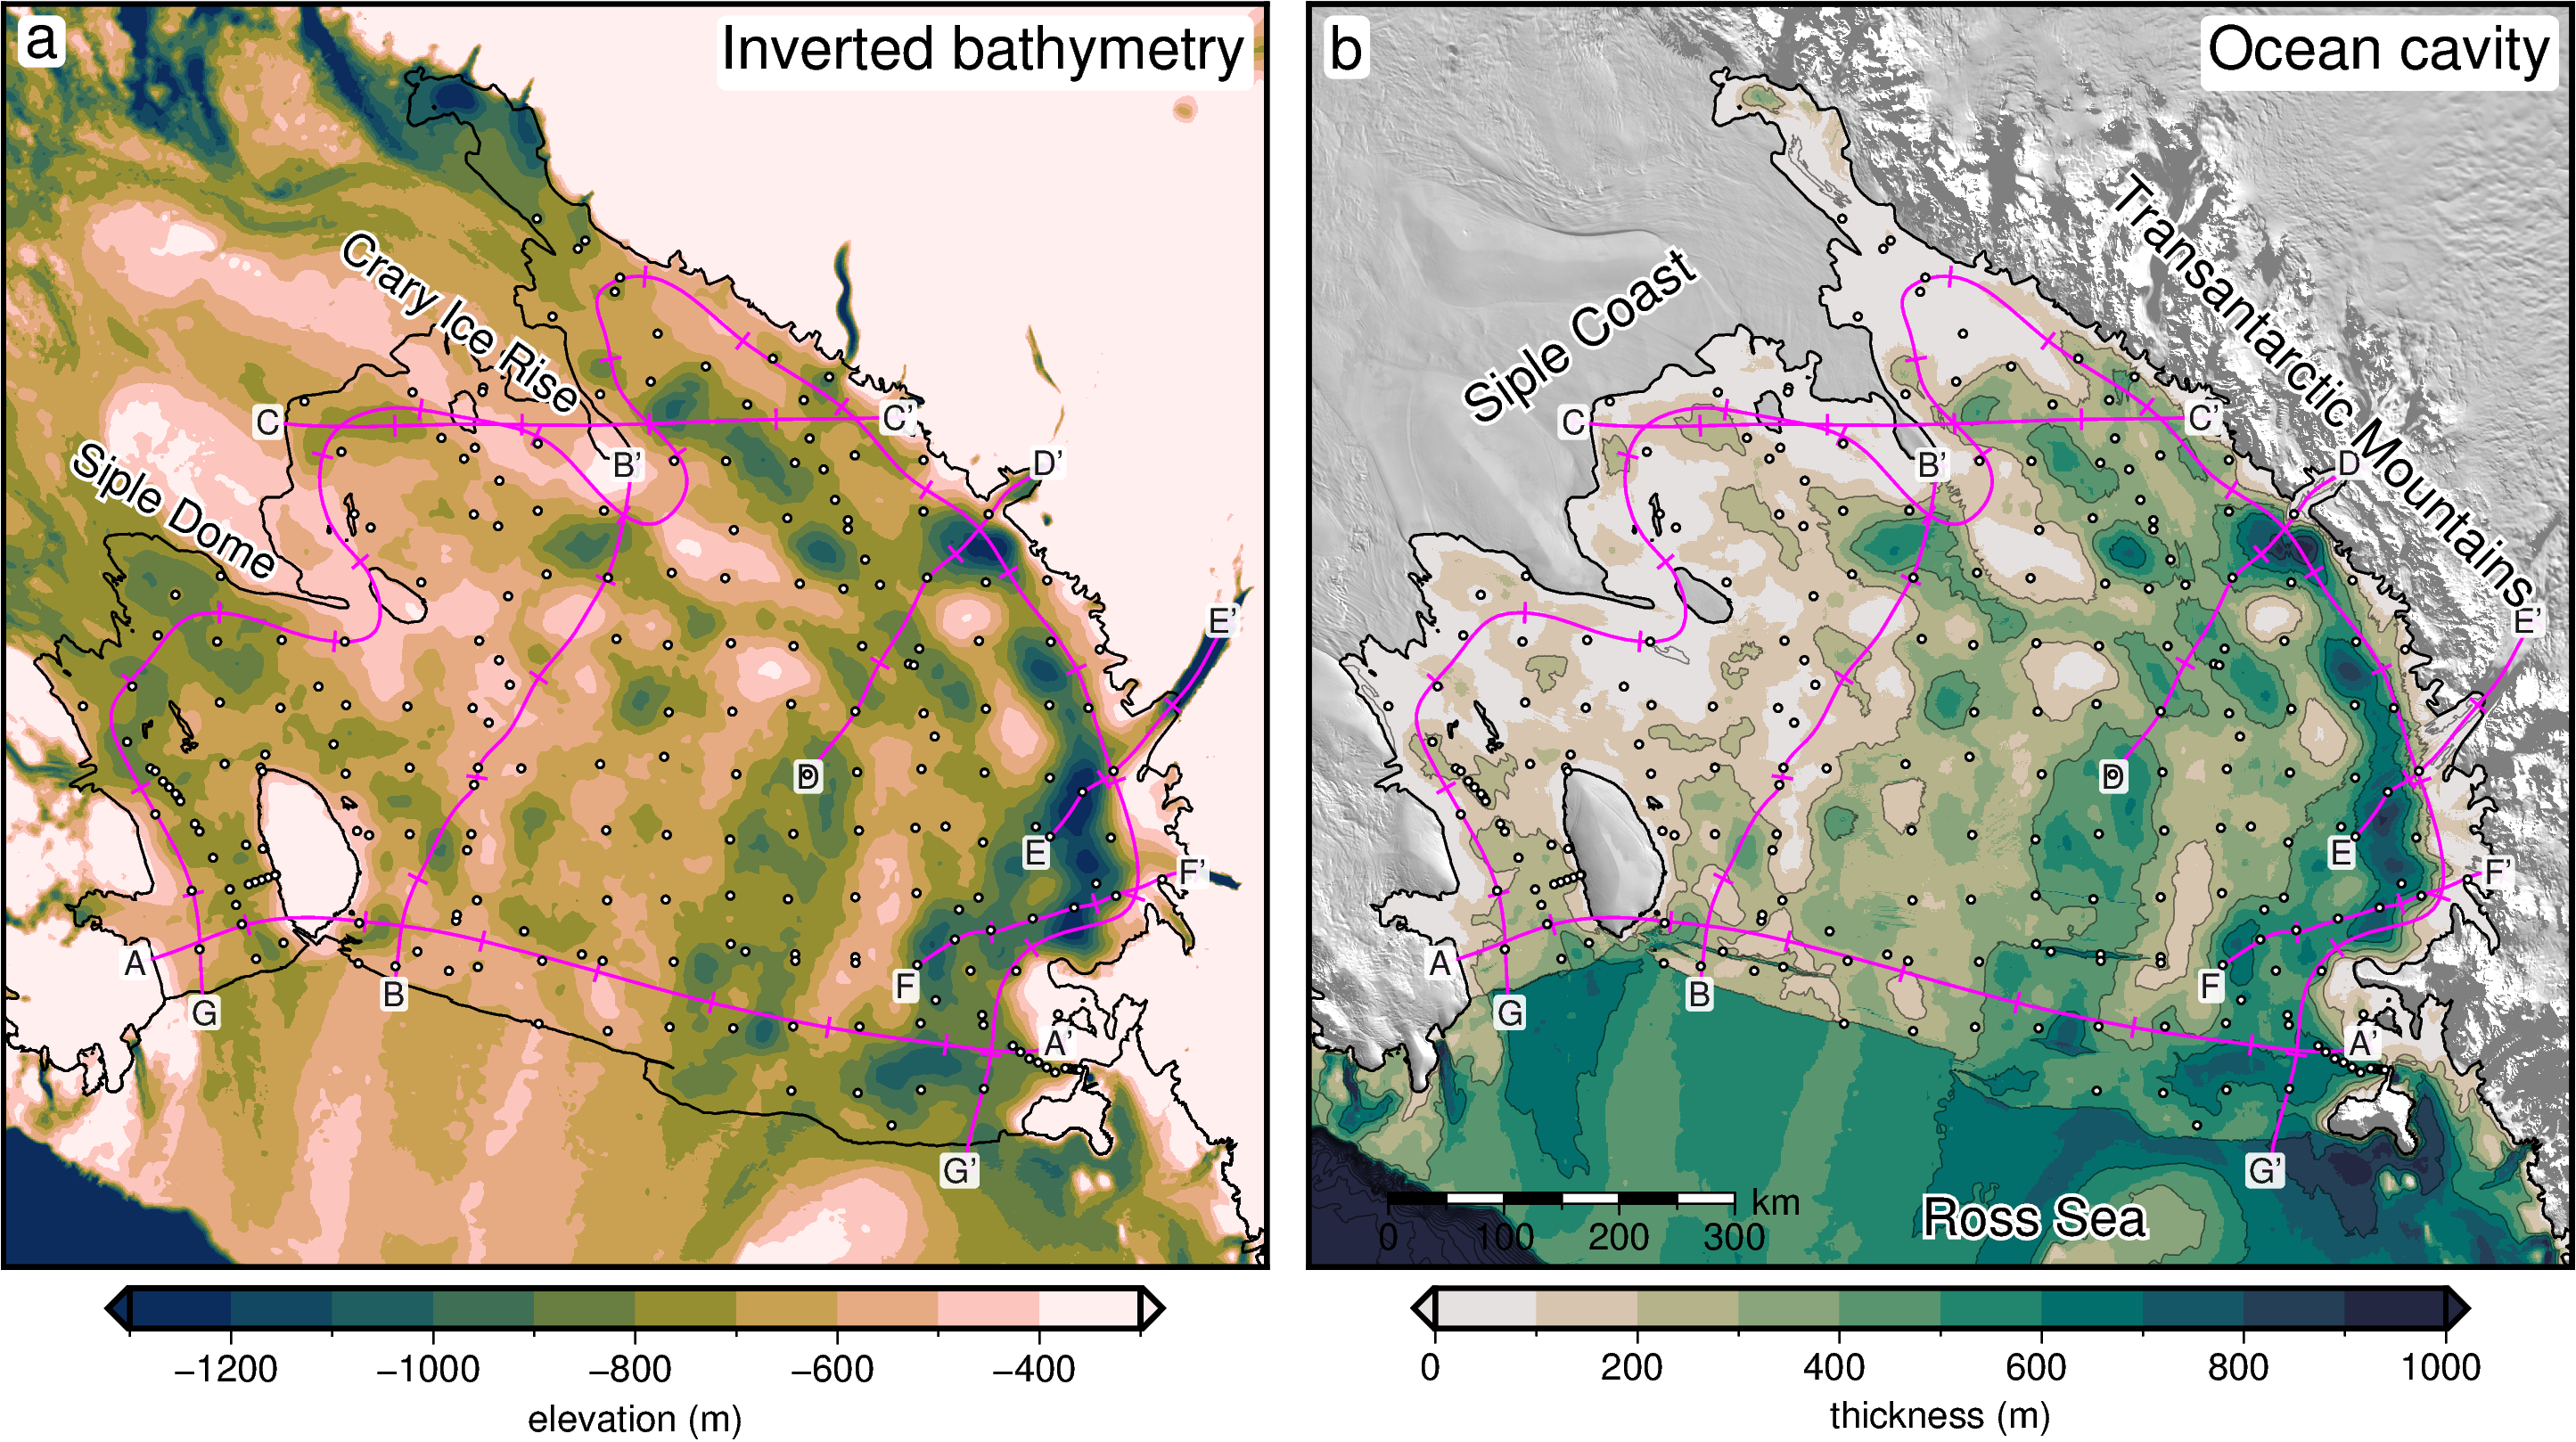
\includegraphics[width=\textwidth]{figures/chp4/RIS_profile_locations.png}
    \end{subfigure}
    
    \makebox[\linewidth][c]{%
    \begin{subfigure}[t]{.6\textwidth}
        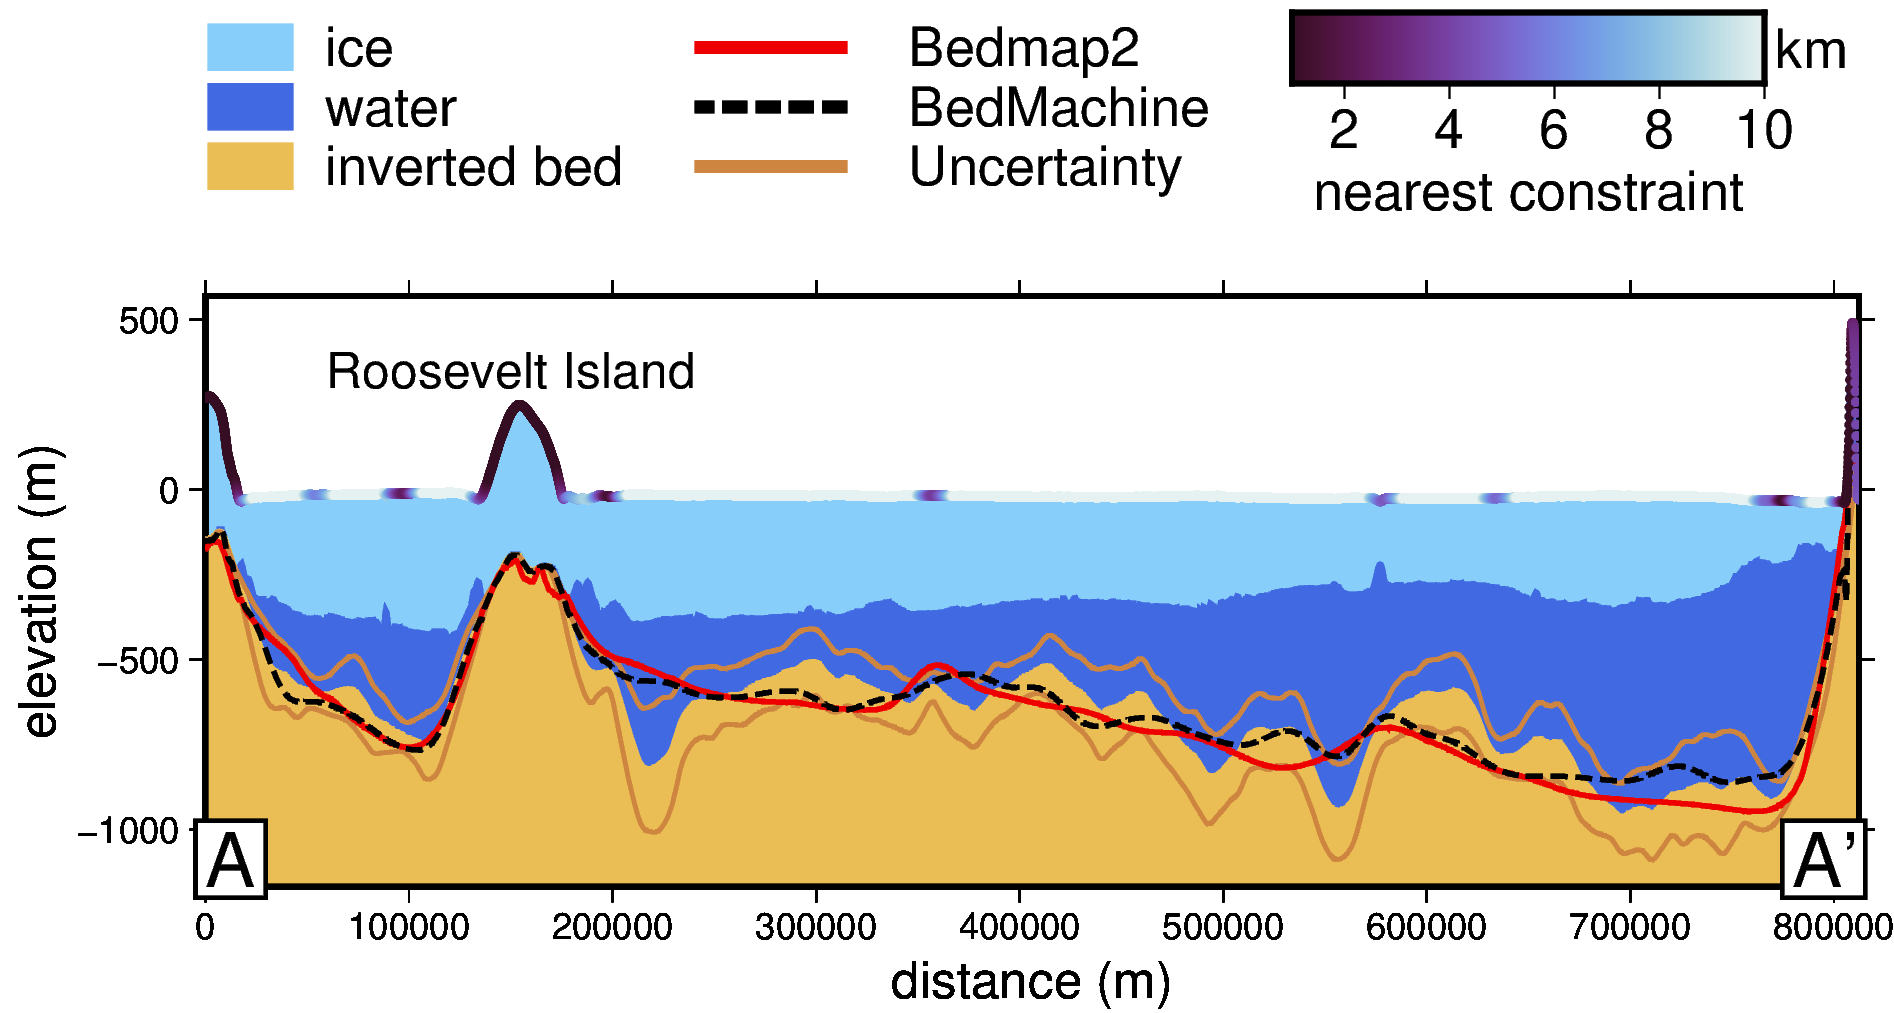
\includegraphics[width=\textwidth]{figures/chp4/profile_A.png}
    \end{subfigure}
    \begin{subfigure}[t]{.6\textwidth}
        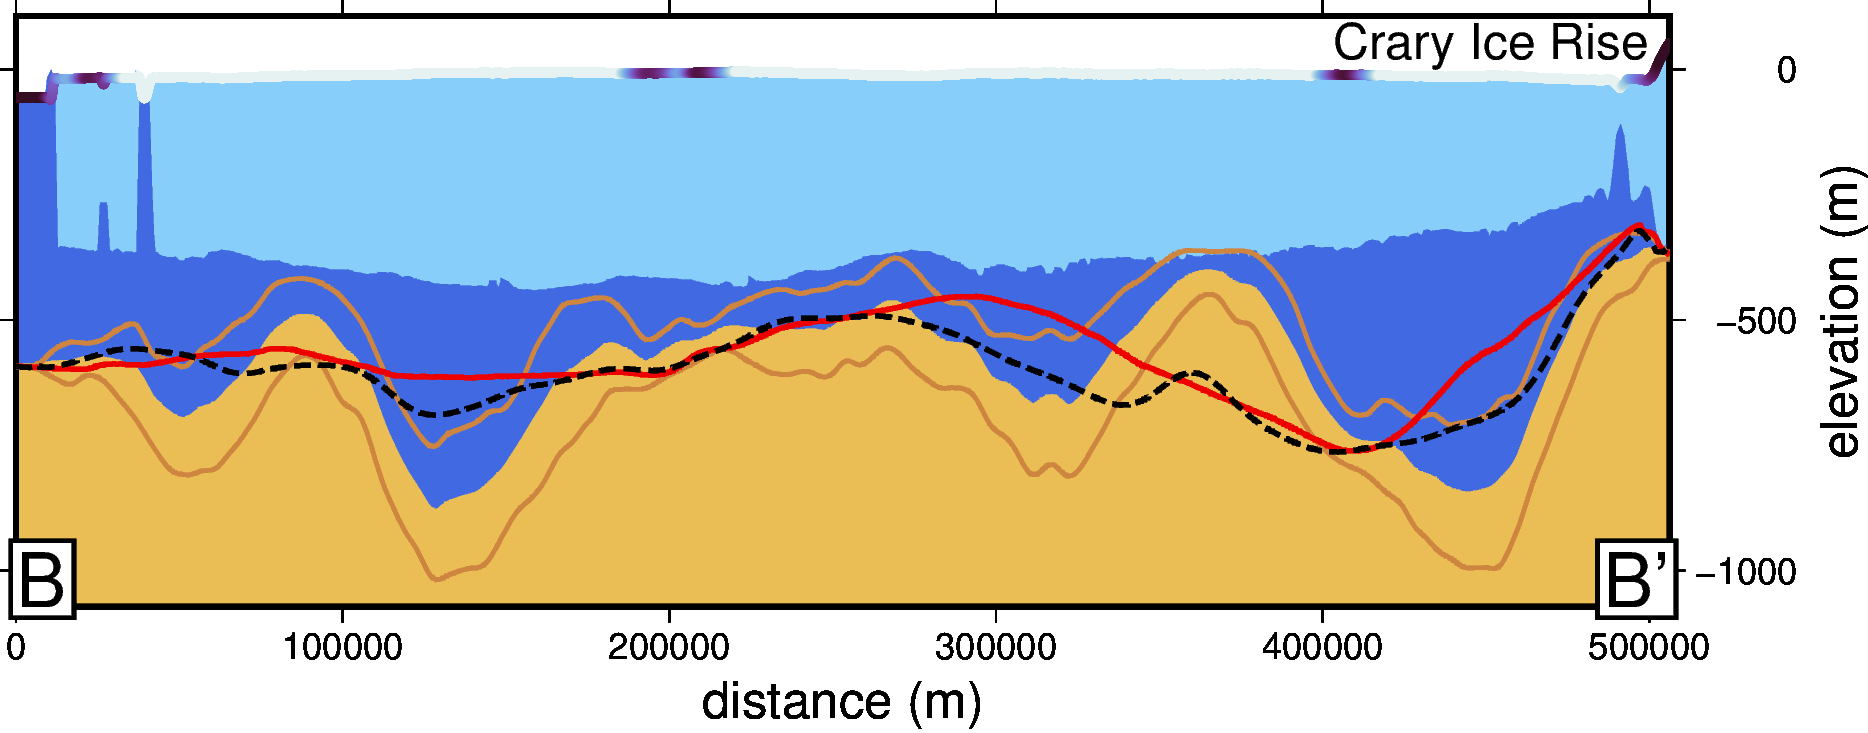
\includegraphics[width=\textwidth]{figures/chp4/profile_B.png}
    \end{subfigure}
    }
    \makebox[\linewidth][c]{%
    \begin{subfigure}[t]{.6\textwidth}
        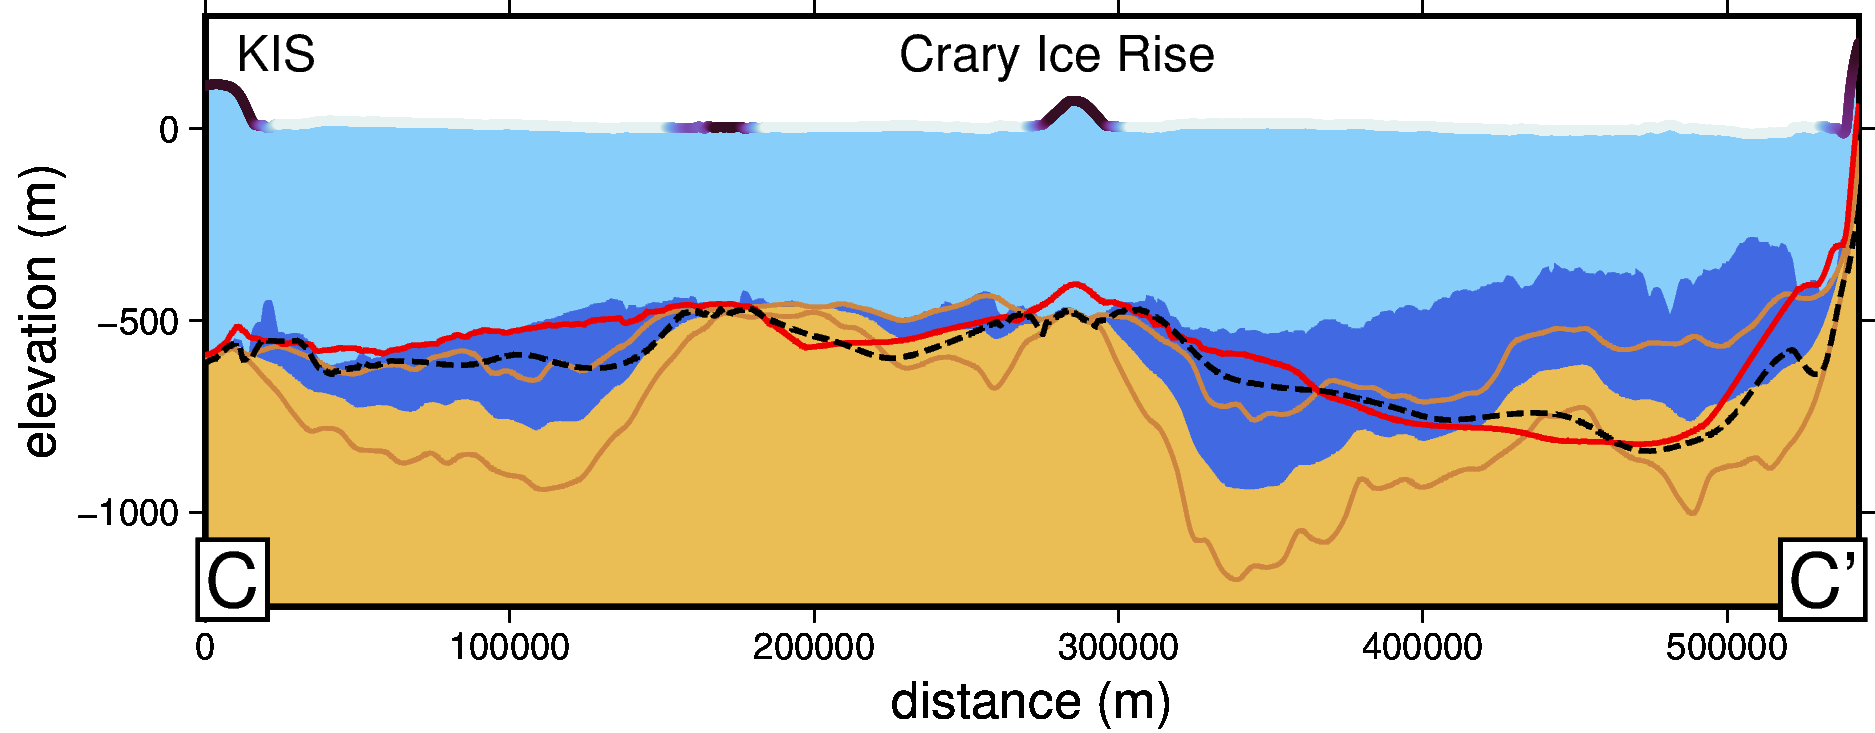
\includegraphics[width=\textwidth]{figures/chp4/profile_C.png}
    \end{subfigure}
    \begin{subfigure}[t]{.6\textwidth}
        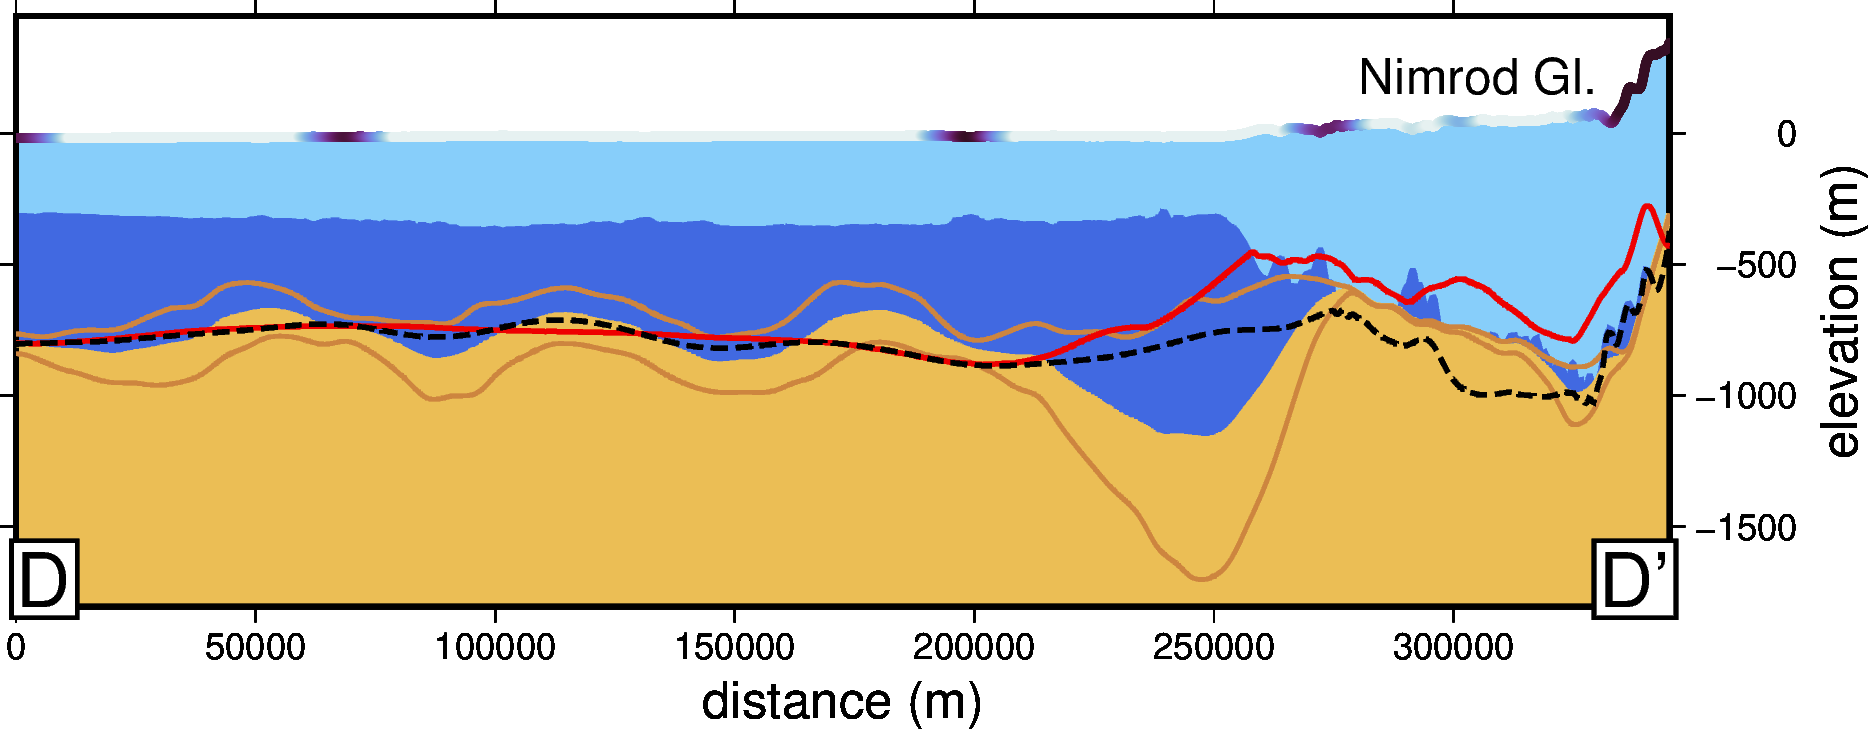
\includegraphics[width=\textwidth]{figures/chp4/profile_D.png}
    \end{subfigure}
    }
    \makebox[\linewidth][c]{%
    \begin{subfigure}[t]{.6\textwidth}
        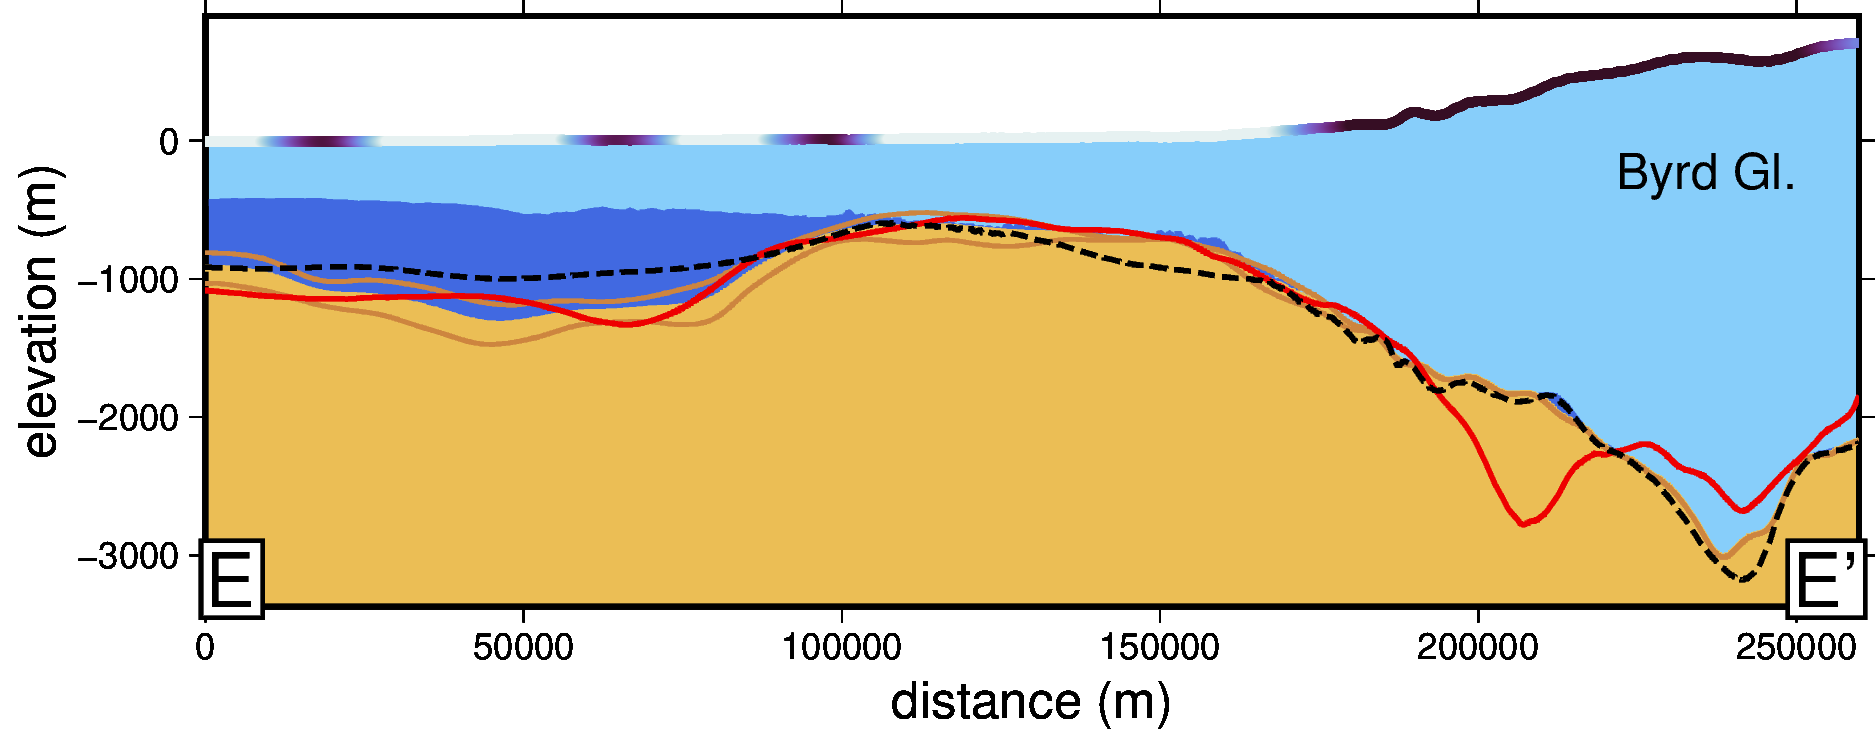
\includegraphics[width=\textwidth]{figures/chp4/profile_E.png}
    \end{subfigure}
    \begin{subfigure}[t]{.6\textwidth}
        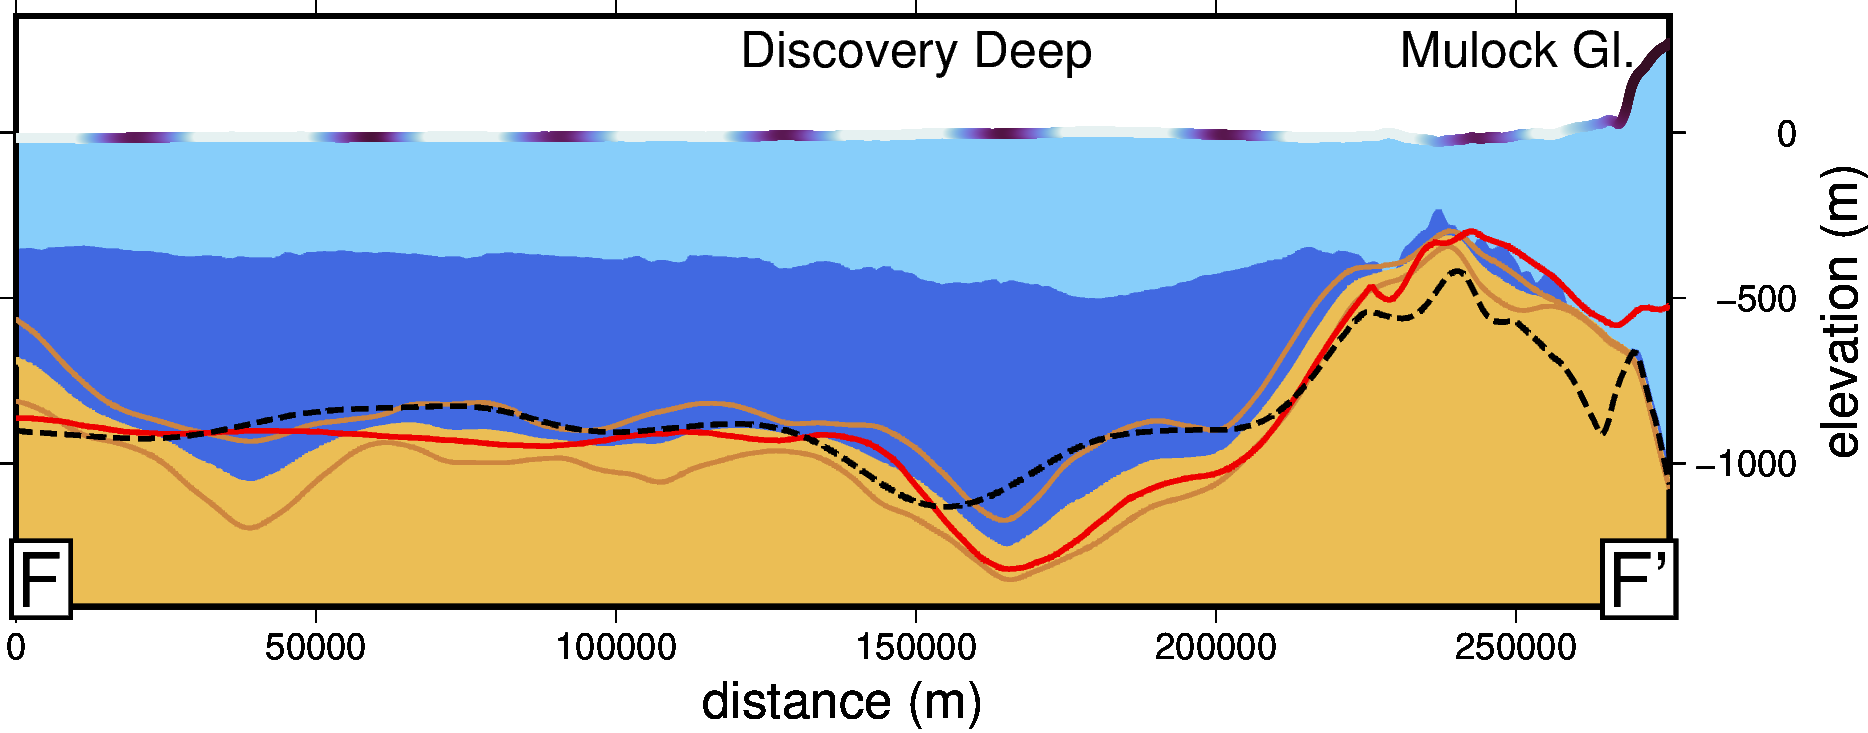
\includegraphics[width=\textwidth]{figures/chp4/profile_F.png}
    \end{subfigure}
    }
    \begin{subfigure}[t]{.95\textwidth}
        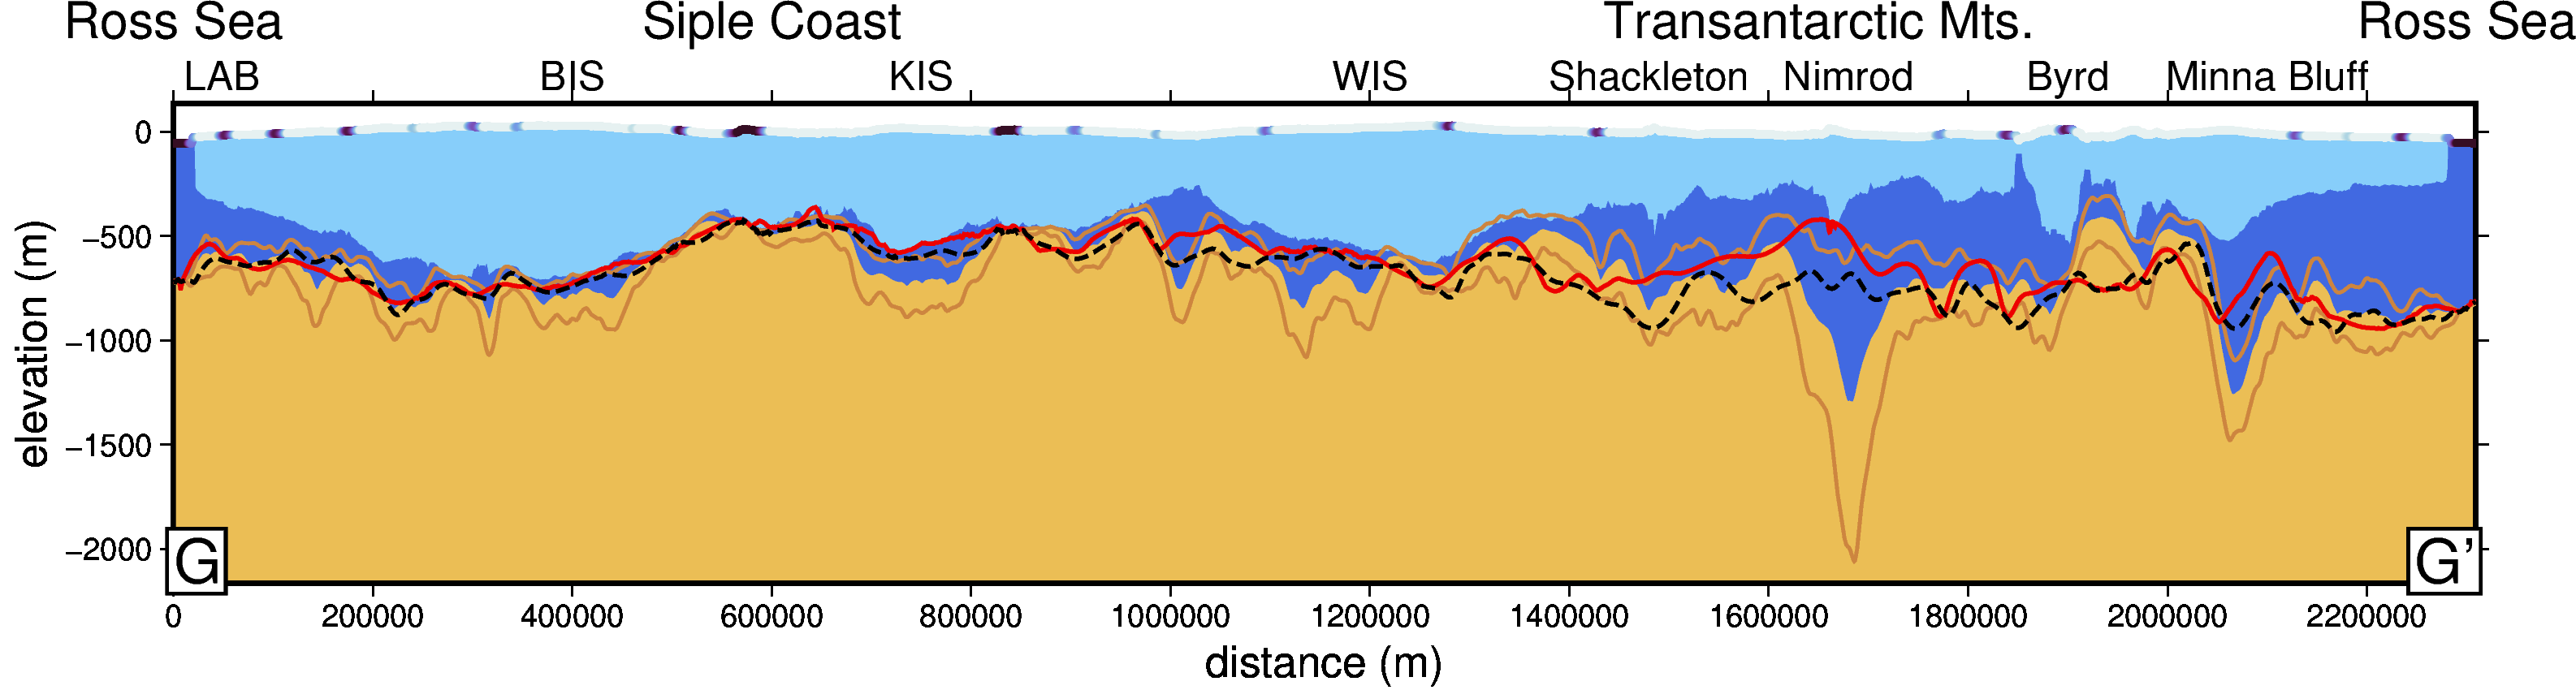
\includegraphics[width=\textwidth]{figures/chp4/profile_G.png}
    \end{subfigure}
    
  \caption[Ross Ice Shelf assorted cross-sections]{\textbf{Upper panel)} Ross Ice Shelf inverted bathymetry (left) and water column thickness (bed to ice base) relative to Bedmachine v3 ice base \citep{morlighemmeasures2022}. Pink lines show profile locations with ticks every $\sim$100~km. Grounding line and coastline in black \citep{mouginotmeasures2017}. Constraint points shown as dots. \textbf{Profiles A-G)} Various cross-sections showing the ice layer (light blue), water layer (darker blue), and bathymetry (yellow), with uncertainties (brown). Red and black lines show Bedmap2 and BedMachine v3 bathymetry, respectively. The colour of the ice surface indicates the distance to the nearest constraint. Legend and colourmap shown above profile A.}
    \label{fig:chp4_RIS_inversion_profiles}
\end{figure}

These shallower depths along the mountain front, instead, could be revealing a flaw in the constraint point minimization assumption of the residual being 0 at constraint points. While the constraint point itself doesn't contribute to the residual signal, since the actual bed is equal to the starting bed at those points, deviations between the actual bed and the starting bed in the vicinity of the constraints may lead to a non-zero residual at the constraint. In this case, the interpolation of the regional field attempts to smoothly connect extremely negative values at the mountain front, and high values at the nearby constraint points. This high gradient leads to poor interpolation. This can be seen in \ref{fig:chp4_RIS_terrain_regional_residual}e where the regional (blue line) is forced exactly equal to the topo-free disturbance (red dashed line) at the constraint point at 700~km along the profile. In reality, the residual gravity at that constraint is likely non-zero. A non-zero value may allow the regional field to more closely match the large positive topo-free disturbance located at 720~km.\\

The remaining major differences between our results and BedMachine v3 include the same series of alternating NW-SE troughs and ridges as discussed above, an $\sim$100~m deeper region on the west side of Roosevelt Island, and a significantly deeper ($\sim$250~m) trough spanning from the south side of Minna Bluff to the outlet of the Byrd Glacier. The greatest depths we model in this trough are $\sim1350\pm100$~m, located offshore of the Byrd Glacier Outlet. Preliminary results of a seismic survey at Discovery Deep, just south of Minna Bluff (cyan line Figure \ref{fig:chp4_RIS_MC_results}), in the 2021/2022 field season report depths up to 1450~m (pers. comm. Prof. A. Gorman). These findings confirm the presence of depths of this magnitude. However, our deepest location is approximately 100~km south of the Discovery Deep survey. These seismic data were not included in this inversion. An additional comparison to a seismic survey can be made proximal to the Kamb Ice Stream grounding zone (cyan line Figure \ref{fig:chp4_RIS_MC_results}). \citet{horganpoststagnation2017} image bathymetry depths along a $\sim20$~km seismic survey with a mean depth of $\sim605$~m. Sampling our bathymetry and uncertainty along this profile yields a mean depth of $\sim608\pm45$~m, while sampling BedMachine v3 bathymetry and uncertainty yields a mean depth of $\sim572\pm79$~m.\\

Comparing the various difference maps of Figure \ref{fig:chp4_RIS_bed_model_comparison} shows that our inversion has resulted in more varied topography across the ice shelf compared to \citet{tintoross2019}. This increased amplitude is likely due to the differences in densities used between the inversions. \citet{tintoross2019} used a spatially variable density model, which ranged from $\sim$2600~-~2800~kg~m\textsuperscript{-3}, with a mean of $\sim$2700~kg~m\textsuperscript{-3}. While we used a spatially-constant density value, in the Monte Carlo analysis the density was varied between $\sim$1800~-~3000~kg~m\textsuperscript{-3}, with a mean of $\sim$2400~kg~m\textsuperscript{-3}. This $\sim$300~kg~m\textsuperscript{-3} difference between the mean density values would result in a more subdued inverted bathymetry from the \citep{tintoross2019} model. While the \citet{tintoross2019} density model does a good job of removing the regional field prior to the inversion, whether or not the density values used are representative of the seafloor is questionable. The lowest values in their model of approximately 2600~kg~m\textsuperscript{-3} represent the upper end of sedimentary rock densities \citep{schöndensity2015}, and are significantly greater than expected densities of unconsolidated sediments. For a region with an expected continuous drape of seafloor sediments \citep[Chapter \ref{ch:2},][]{tankersleybasement2022}, we expect the densities used in \citep{tintoross2019} were too high. This explanation for the differences between the inversion results is supported by the strong correlation between our bathymetry uncertainty resulting from the choice in density (Figure \ref{fig:chp4_RIS_MC_sensitivity}c) and the difference between the inversion results (Figure \ref{fig:chp4_RIS_bed_model_comparison}f). This shows the importance of picking a plausible density value, and the added benefit of testing many values to estimate the uncertainty related to the chosen density value. \\


\subsubsection{Ocean cavity comparison}

Due to the smoothness of the base of an ice shelf, relative to bathymetry, the water column thickness beneath many ice shelves is predominately determined by the bathymetry. We use BedMachine v3 ice base elevations and our updated bathymetry to calculate the water column thickness beneath the Ross Ice Shelf and compare the results to the water column thicknesses of Bedmap2 and BedMachine (Figure \ref{fig:chp4_RIS_ocean_draft_comparison}). These differences are very similar to those described above, due to the smooth nature of the ice base. Notable areas where our results show a thicker ocean cavity (within uncertainty ranges) compared to past models include;
\begin{enumerate}
    \item 
    Nearby the Kamb grounding zone ($\sim100\pm50$~m thicker, Figure \ref{fig:chp4_RIS_inversion_profiles}c near km 100).
    \item 
    The west side of Crary Ice Rise ($\sim300\pm150$~m thicker, Figure \ref{fig:chp4_RIS_inversion_profiles}c near km 350).
    \item 
    The south side of Minna Bluff ($\sim300\pm200$~m thicker, Figure \ref{fig:chp4_RIS_inversion_profiles}g near km 2100).
    \item 
    The west side of Roosevelt Island ($\sim200\pm100$~m thicker, Figure \ref{fig:chp4_RIS_inversion_profiles}a near km 220)).
\end{enumerate}

Notable areas where our results show a thinner cavity include;
\begin{enumerate}
    \item 
    The mountain front north of Byrd Glacier ($\sim300\pm50$~m thinner, Figure \ref{fig:chp4_RIS_inversion_profiles}g near km 2000)).
    \item 
    Three 50~km wide regions in the central ice shelf, which are up to $200\pm50$~m thinner.
    \item 
    Several points approximately 50~km off of the Transantarctic Mountain front which are up to $400\pm50$~m thinner (Figure \ref{fig:chp4_RIS_inversion_profiles}c near km 450).
\end{enumerate}

\begin{figure}[!ht]
    \centering
    \includegraphics[width=.98\textwidth]{figures/chp4/RIS_ocean_draft_comparison.png}
    \caption[Water column thickness comparisons]{Comparison of our updated water column thickness with past models. \textbf{a)} Difference between our model and the water column thickness from Bedmap2, and \textbf{b)} the Bedmap2 water column thickness. \textbf{c)} Water column thickness calculated as the difference between BedMachine v3 icebase and our inverted bathymetry. \textbf{d)} Difference between our model and the water column thickness from Bedmachine v3, and \textbf{e)} the Bedmachine v3 water column thickness. Blue regions in the difference maps indicate where our results' water column is thinner, while red regions indicate where our results are thicker than the past models. Grounding line and coastline are shown in black \citep{morlighemmeasures2022}. Background imagery is from \citet{scambosmodisbased2007}. Water column thickness grids are contoured at 200~m intervals, and the 20~m contour is shown in bright blue. The difference grids are contoured at 100~m intervals. Water column thickness grids and difference grids share common colour scales.}
    \label{fig:chp4_RIS_ocean_draft_comparison}
\end{figure}

\subsection{Implications}

Here, we discuss several of the important implications of our updated sub-RIS bathymetry. These implications relate to the stability of the Ross Ice Shelf, geology, and tectonics. 

\subsubsection{New potential pinning points}

We have identified several areas of thin water column thickness ($<20$~m) with our updated results beneath the Ross Ice Shelf. These areas are shown by the 20~m water column thickness contour, in bright blue in Figure \ref{fig:chp4_RIS_ocean_draft_comparison}a. These include a $\sim$100x100~km region SW of Roosevelt Island, several $\sim$50x50~km regions on the north flank of Crary Ice Rise (Figure \ref{fig:chp4_RIS_inversion_profiles}g at km~$\sim900$), and a widespread region south of Crary Ice Rise (Figure \ref{fig:chp4_RIS_inversion_profiles}g at km~$\sim1350$). Thin water depths south of Crary Ice Rise have also been modelled by a local gravity survey along the Whillans Ice Stream grounding zone \citep{mutobathymetry2013}. Additionally, two smaller regions of sub-20~m water column thickness are found nearer the centre of the ice shelf. One is approximately 100~km off the point of Crary Ice Rise and is $\sim400$~km\textsuperscript{2} (Figure \ref{fig:chp4_RIS_inversion_profiles}c at km~$\sim200$). The second is $\sim200$~km north of Crary Ice Rise and is slightly smaller (Figure \ref{fig:chp4_RIS_inversion_profiles}b at km~$\sim350$). None of these shallow water column regions are present in either of the past models. Interestingly, these regions coincide with some of the lowest uncertainties we report $\sim20$~m. A portion of this low uncertainty may be related to the inversion constraining the bathymetry to the ice base, which in regions of thin water column will reduce the variability of the suite of inversions in the Monte Carlo simulation which were used to define the uncertainty.\\

These newly-identified shallow regions highlight where the Ross Ice Shelf was likely grounded in the recent past, or could likely become re-grounded in the future. While some of these regions are small, analysis of pinning points on the Ross Ice Shelf has shown some of the smallest pinning points can create the largest effective resistance on the ice shelf \citep{stillmechanical2019}. Additionally, some of these locations (north side of Crary Ice Rise) are predicted to have on the order of 1~m/yr of basal accretion \citep{adusumilliinterannual2020}. An already thickening shelf within $\sim$20~m of the bed will likely affect the ice sheet dynamics as part of future projections of the ice shelf. Incorporation of these localities of likely past pinning points may aid in resolving the ongoing debate of the style of grounding line retreat and readvance of the Ross Ice Shelf throughout the Holocene \citep{venturellimid2020, kingslakeextensive2018, lowrydeglacial2019}.\\ 


\subsubsection{Basal melting}

\begin{figure}[!ht]
    \centering
    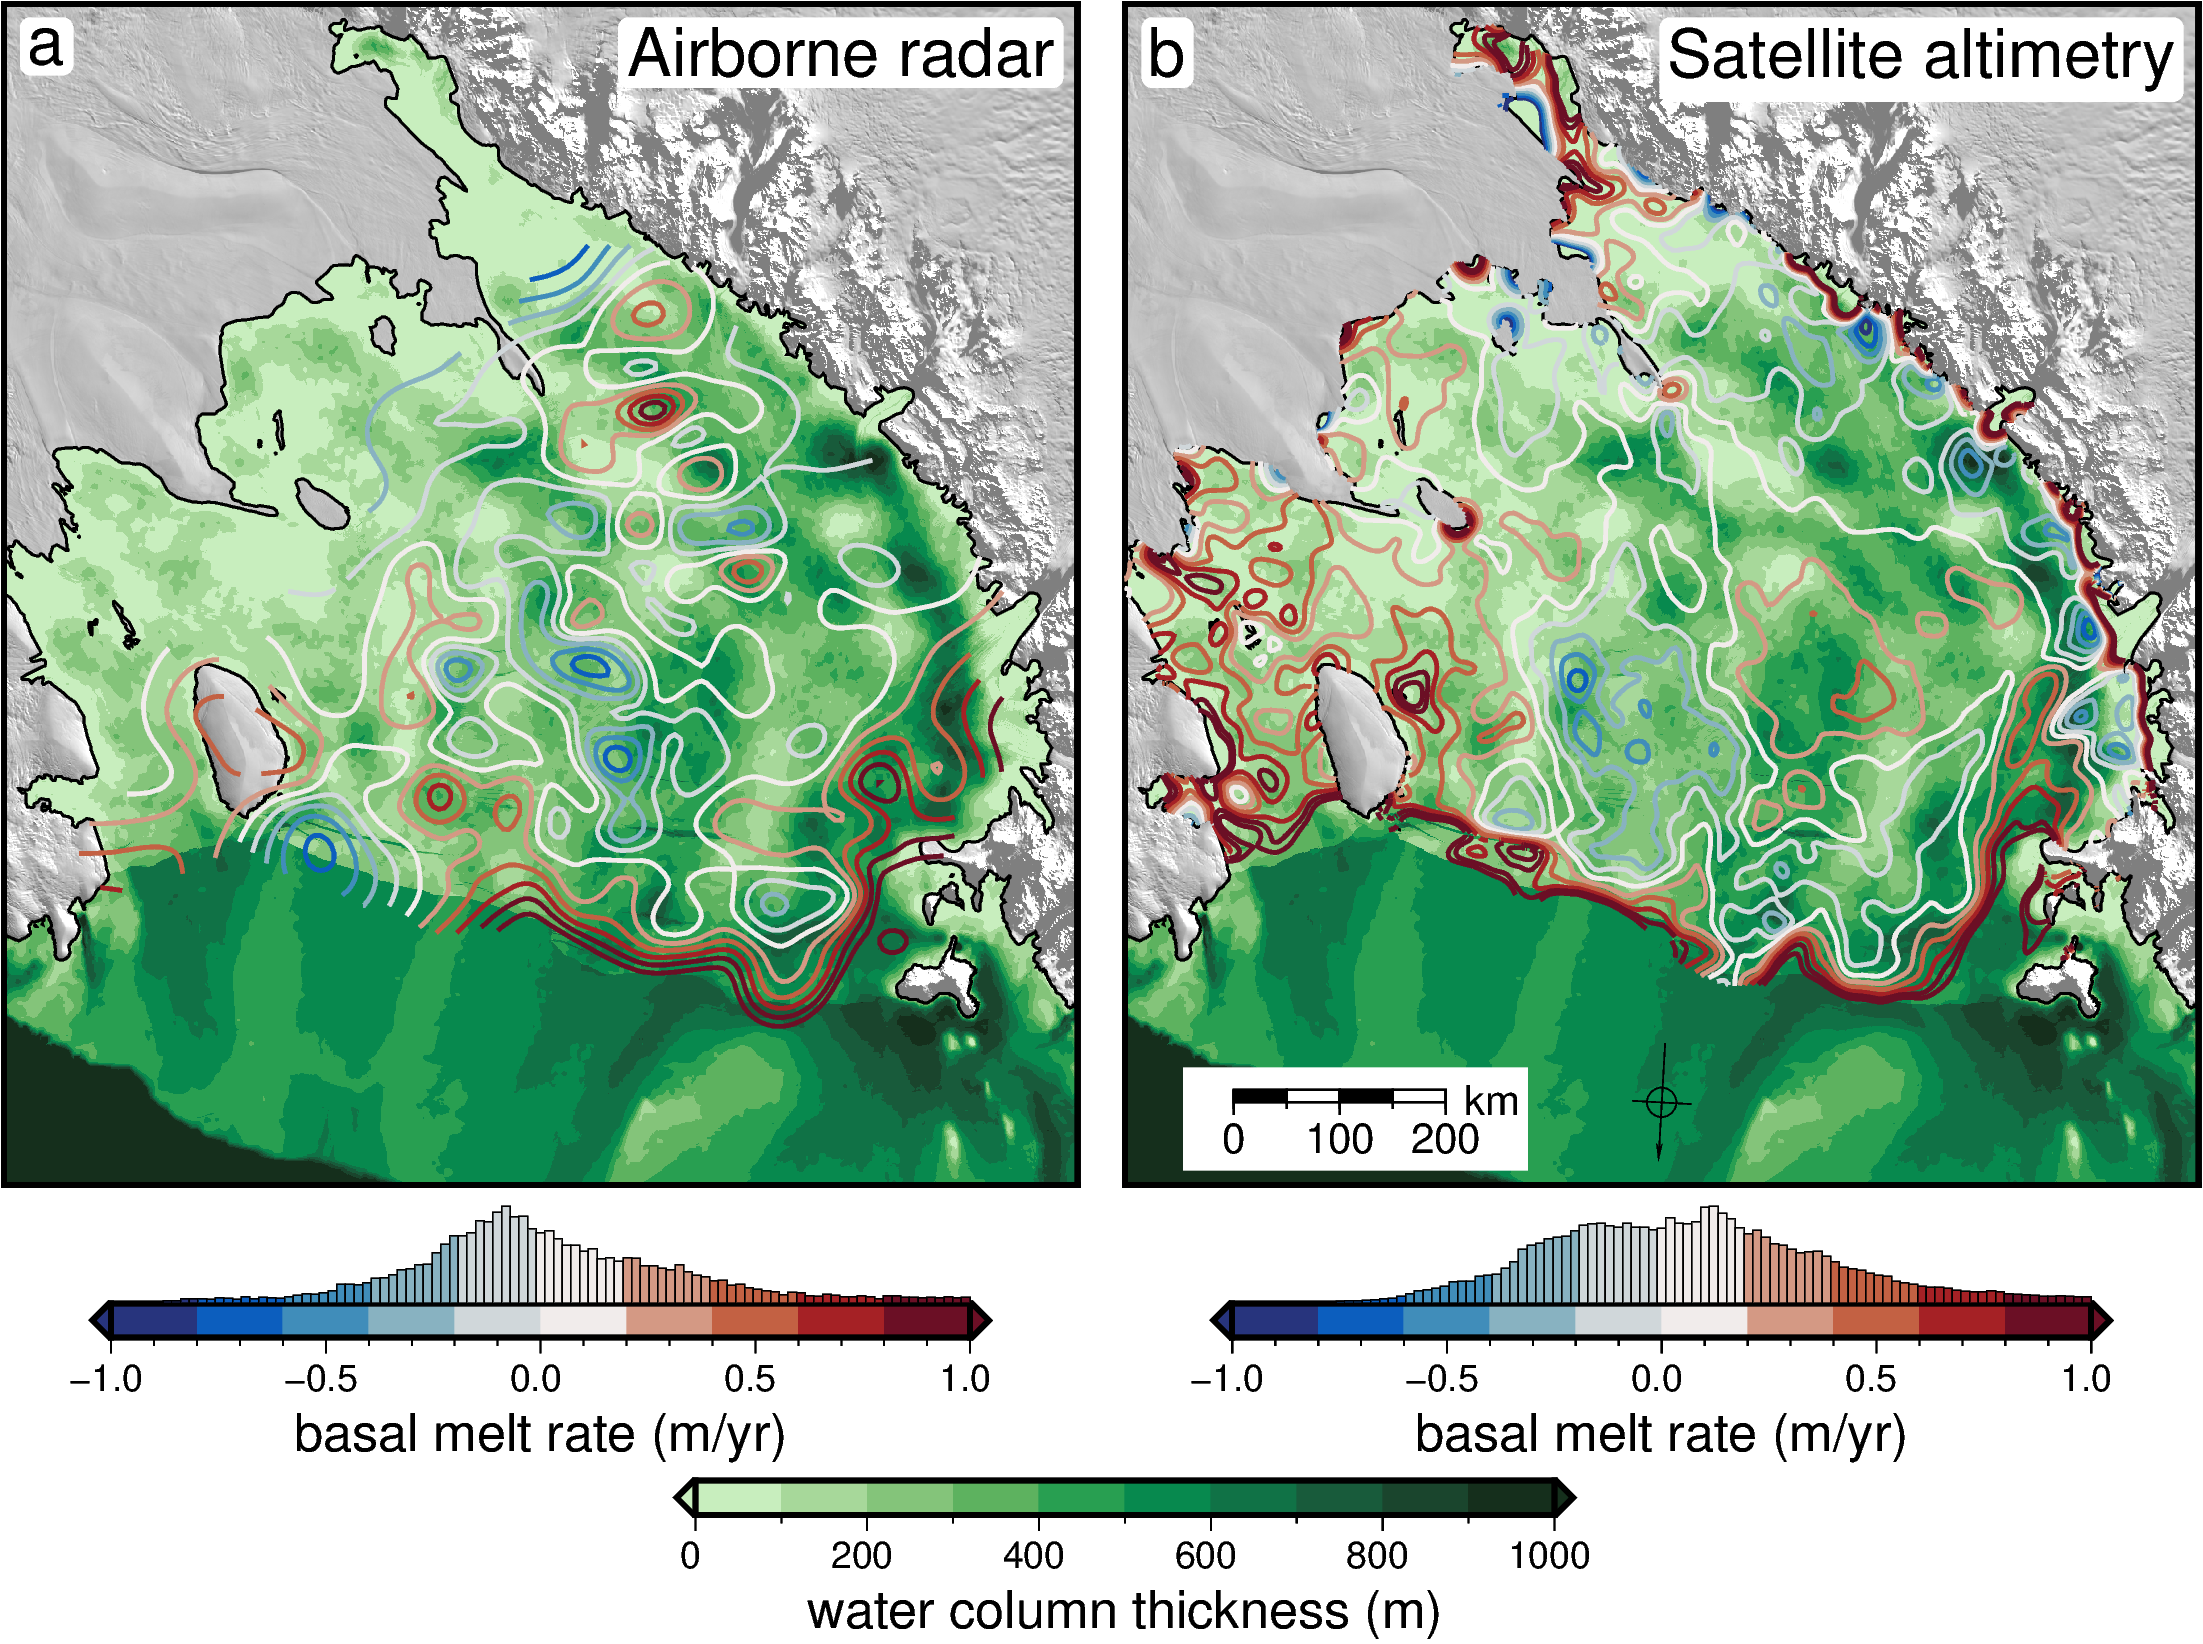
\includegraphics[width=0.95\textwidth]{figures/chp4/RIS_basal_melt.png}
    \caption[Basal melt]{Basal melt rate and water column thickness compared for the Ross Ice Shelf. \textbf{a)} Blue to red contours show interpolated basal melt rate from \citet{dasmulti2020} derived from ROSETTA-ice airborne ice-penetrating radar. Background shows water column thickness from this study. \textbf{b)} Same as \textbf{a} but with basal melt rate from \citet{adusumilliinterannual2020} derived from satellite altimetry. Black line is the grounding line from \citet{mouginotmeasures2017}. Background imagery is from MODIS-MOA \citep{scambosmodisbased2007}.}
    \label{fig:chp4_basal_melt}
\end{figure}

Our updated bathymetry, water column thickness, and uncertainty maps provide additional information vital to understanding the distribution of basal melt beneath the ice shelf. Melt beneath the Ross Ice Shelf is thought to predominantly occur 1) along the ice front, where Antarctic Surface Water causes rapid melting in the summer \citep[Figure \ref{fig:chp4_basal_melt}][]{horgansurface2011, moholdtbasal2014}, and along the deep grounding zones of the Transantarctic Mountain front, where contact with High Salinity Shelf Water induces melting \citep[Figure \ref{fig:chp4_basal_melt}b][]{tintoross2019, adusumilliinterannual2020}. Throughout the centre of the ice shelf are zones of refreezing \citep[Figure \ref{fig:chp4_basal_melt}][]{dasmulti2020, adusumilliinterannual2020}. Overall basal melting of the Ross Ice Shelf is thought to be low compared to other shelves due to the blocking of warm Circumpolar Deep Water from entering the cavity. This blocking is from a layer of dense High Salinity Shelf Water \citep{tintoross2019, dinnimanmodel2011}. The Hayes Bank (Figure \ref{fig:chp4_inversion_inputs}b) has been identified  as one location where the Circumpolar Deep Water is able to penetrate the ice shelf cavity and induce melting, but this penetration is thought to be limited to the region near Roosevelt Island \citep{tintoross2019, dasmulti2020}. Our ocean cavity is $\sim100$~m thicker than \citet{tintoross2019} immediately to the west of Roosevelt Island (Figures \ref{fig:chp4_RIS_inversion_profiles}a and \ref{fig:chp4_RIS_ocean_draft_comparison}d). This region should be investigated with sub-shelf circulation models using our updated bathymetry. Our larger cavity allowing the inflow of warm Circumpolar Deep Water beyond Roosevelt Island could help explain the relatively large basal melt rate found in the region as shown by satellite altimetry (Figure \ref{fig:chp4_basal_melt}b).\\

The high melt rates measured along the Transantarctic Mountain front \citep{adusumilliinterannual2020} are caused by the inflow of High Salinity Shelf Water \citep{tintoross2019}. This water is thought to be guided by bathymetric troughs and is able to induce melting only at large depths, due to the pressure suppression of the melting temperature of ice. Figures \ref{fig:chp4_basal_melt} show a comparison of both airborne radar and satellite altimetry-derived basal melt rates to the updated water column thickness resulting from our bathymetry inversion. The deeper bathymetry proximal to the Transantarctic Mountain front found in both our inversion and \citet{tintoross2019}, compared to the depths of Bedmap2, help explain the high melt rates measured there. The other locations we report with deeper bathymetry near grounding zones, such as the south side of Minna Bluff, and the far southern end of the ice shelf, at the Mercer Ice Stream grounding zone, may be potential locations where High Salinity Shelf Water is able to induce basal melt. Additionally, some of the very shallow water column thicknesses ($<20$~m) we find (Figure \ref{fig:chp4_RIS_ocean_draft_comparison}c), for instance to the south of Crary Ice Rise, correspond with low basal melt rates (Figure \ref{fig:chp4_basal_melt}). This may be due to the lack of stratification in the water column, which occurs due to tidal mixing possible only in thin water columns \citep{mutobathymetry2013, hollandmodel2008}.


% RIS
% RIS show high melt rates under deep ice drafts near GZ and shallow ice drafts near ice front, separated by zones of refreezing \citep{adusumilliinterannual2020}
% most RIS melting at ice drafts between 250 and 750m \citep{adusumilliinterannual2020}
% recent stability of RIS due to insulation of cavity from warm CDW intrusions by cold dense water masses  \citep{tintoross2019, dinnimanmodel2011}
% 25-30\% of total mass loss from basal melt \citep{rignoticeshelf2013}
% mCDW flows south at Hayes Bank to ice front, melting hotspot \citep{dasmulti2020}

% GZ
% RIS basal mass loss driven by cold, High Salinity Shelf Water melting near GZ 
% ocean modelling suggest melt rates are less variable at deep GZ sinze driven by stable circulation of HSSW \citep{tintoross2019}
% ICE FRONT
% 10-40\% sub-RIS melt within 40km of ice front \citep{horgansurface2011}
% ice shelf front melt less important than at grounding since it is within passive ice zones 
% \citep{adusumilliinterannual2020}

% BATHY
% no direct relation between cavity thickness and melting \citep{goldbergbathymetric2020, derydtgeometric2014}
% seabed ridge (300 m )blocks deep and warm waters from reaching thickest ice in Pine Island Glacier. Ridge enhances PIG's sensitivity to oceanic and therefore climatic forcing, by \citep{dutrieuxstrong2014, derydtgeometric2014} 
% similar to entrance sill offshore of ice front at Jakobshavn Glacier

% thin water is tidally mixed, not statified, and therefore has slower basal melting \citep{mutobathymetry2013, holland2008}

% in general grounding line is deeper than bedmap2
% Whillans and Mercer has shallower grounding zones and thinner ocean drafts. 
% 400 m deeper at Nimrod glacier grounding zone Figure \ref{fig:chp4_RIS_inversion_profiles}d 
% 200 m deeper at Mulock glacier grounding zone


\subsubsection{Geologic and tectonic significance}

While there are many interesting implications to explore in this new dataset, we limit our discussion to several sub-Ross Ice Shelf bathymetric features of possible importance to solid-Earth investigations. These features include the bathymetry along the Transantarctic Mountain front, a deep feature on the southwest flank of Crary Ice Rise, and a newly identified orientation of bathymetry features, aligned with the Siple Coast ice streams. 

\paragraph*{Transantarctic Mountain front}

The Transantarctic Mountains (Figure \ref{fig:chp4_inversion_inputs}a) make up the world's largest rift shoulder. Despite their prominence, the uplift mechanisms are still debated \citep{goodgegeological2020}. It is likely that these mechanisms vary along-strike, and consist of some combination of thermal, flexural, or isostatic support \citep{goodgegeological2020}. For the central TAM, a mechanism of cantilevered flexure is proposed for the uplift of the mountains \citep{wannamakeruplift2017, yamasakinumerical2008}. This theoretically should be accompanied by a deep trough parallel just offshore the range front, and an outer bathymetric high, approximately 200 km from the range front \citep{sternflexural1989}. These features have not yet been observed \citep{tenbrinkgeophysical1993, wannamakeruplift2017}. Our results show a deep trough along the range front between the Nimrod Glacier and Minna Bluff, with bathymetry highs further offshore. These features may support the theory of flexural uplift along this portion of the TAM \citep{wannamakeruplift2017}. Further south, where the trough disappears, the mechanism of flexural uplift is not required, since the mountains have a crustal root, which likely provides the uplift mechanism, via Airy isostasy \citep{blockantarctic2009, wannamakeruplift2017}. 

% support lithospheric foundering and the associated thermal support are proposed for the southern TAM \citep{shenseismic2018}, mechanical support through a cantilevered flexure mechanism is proposed for the central TAM \citep{wannamakeruplift2017}, and thermal support associated with a high-temperature anomaly of the upper mantle is suggested for the vicinity of Ross Island \citep{olivettivariability2018}. 

% MT survey \citep{wannamakeruplift2017} shows highly resistive lithosphere of upper mantle, eliminating thernal load possibility, and suggests cantilevered flexure for uplift of CTAM, but lack of hangingwall flexural trough is not observed \citep{tenbrinkgeophysical1993}

\paragraph*{Fault bound Crary Ice Rise}

Figure \ref{fig:chp4_RIS_inversion_profiles}c shows a profile of the updated bathymetry model across the Crary Ice Rise. Our results show a steep drop off the south flank of the ice rise (at km $\sim320$), to depths up to $\sim1000\pm200$~m. This steep drop-off is aligned with an NW-SE fault proposed by \citet{mutobathymetry2013} from a local gravity survey along the Whillan Ice Stream grounding zone. Depth to basement analysis from magnetic data \citep[Chapter \ref{ch:2},][]{tankersleybasement2022} also highlights this north flank of Crary Ice Rise as a likely location for faults. We believe this steep bathymetry feature adds evidence to the proposition of the Crary Ice Rise as a fault-bound horst \citep{mutobathymetry2013}. This would imply the current grounding of the Ross Ice Shelf along the Crary Ice Rise is in part controlled by regional tectonics. 

\paragraph*{New bathymetric trend}

From the gridding of point data, the bathymetry of the central Ross Ice Shelf is dominated by an N-S~-~NNE-SSW trend, aligned with the flow directions of the outlet glaciers of the Transantarctic Mountains (Figure \ref{fig:chp4_inversion_inputs}). Our updated bathymetry model (Figure \ref{fig:chp4_RIS_MC_results}a) adds an overprinted NW-SE trend to the bathymetry features of the central portion of the ice shelf. This trend is prevalent, but subtle, in the inversion of \citet{tintoross2019}. The features comprising this trend are a series of 2-3 ridges and troughs of $\sim100$~m amplitudes and $\sim50$~km wavelengths, as shown in Figure \ref{fig:chp4_RIS_inversion_profiles}d. These features are oblique to flight lines, adding to their validity, and are well-aligned with the Crary Ice Rise and the general ice flow direction of the Siple Coast ice streams. This trend could signify several things; 1) the most recently grounded ice in this region had a flow direction aligned with the Siple Coast ice streams, leaving behind erosional or depositional features with these orientations, 2) these features are tectonic in origin, and are the surface expressions of rift structures. These structures overprint the large bathymetric depression which runs from the Nimrod glacier to the calving front. If these are features left behind from the most recent grounding line retreat, they might inform the style of retreat. As seen in the Ross Sea, physiography of the sea floor exerts the primary control on ice stream flow and the patterns of retreat \citep{halberstadticesheet2016}. 


% \begin{itemize}
%     \item Bathymetry features
%         \begin{itemize}
%             \item \sout{shallow zones can reground to become ice rises / rumples, providing added resistance}
%             \item \sout{new shallow zones as past pinning points}
%             \item \sout{trough along TAM, related to flexure?}
%             \item \sout{Steep dropoff at CIR (Muto et al. faulting?}
%             \item Byrd and Nimrod troughs, Byrd is very sharp
%             \item deeper at glacier inlets (byrd, nimrod, beardmore, skelton)
%             \item generally all grounding line is deeper
%             \item majority of calving front is shallower
%             \item Minna bluff is all deeper (loading?)
%             \item new deepest point at Disco Deep (confirmed by 2022 surveying)
%             \item bedrock plateaus \citep{wilsonbedrock2006}
%         \end{itemize}
%     \item Ocean draft
%         \begin{itemize}
%             \item thinner along siple coast
%             \item thinner at calving front
%             \item compare sat-derived melt rates, ROSETTA melt rates, and ocean cavity
%             \item Baldachnio for sensitivity analysis
%         \end{itemize}
%     \item Analysis of resulting Topo-Free disturbance
%         \begin{itemize}
%             \item low gravity around Roosevelt?
%             \item Relationship between gravity data and bathymetry, karner et al 2005.
%             \item  Disco deep low offset from gravity high
%             \item majority of gravity signal not reflective of bathymetry, shows likely crustal features
%         \end{itemize}
% \end{itemize}

% \subsection{Future work}

% apply noise to entire lines, and redo interpolation, instead of adding noise to individual points of the gridded data

% Larsen C is a good candidate for an inversion 
% - largest on the AP
% - past inversions were very uncertain \citep{cochraninversion2012}
% - new compilation of seismic data \citep{brisbourneupdated2020, }

% \begin{enumerate}
%     \item incorporate ground-based gravity surveys into the input observed gravity data
%     \item use satellite gravity to re-level the ROSETTA flight lines
%     \item use cross-validation to choose best density value
% \end{enumerate}

% inversion can be used on grounded ice as well

\section{Conclusion}

Here we present an updated model of bathymetry depths beneath Antarctica's Ross Ice Shelf, as modelled from airborne gravity data. Our inversion algorithm provides a comprehensive spatial uncertainty analysis and parameter sensitivity estimation. This uncertainty highlights regions of high uncertainty that would benefit from additional seismic constraints. These regions include the entire Transantarctic Mountain front and two points near the centre of the shelf which are up to 40~km from the nearest constraints. We summarize some key findings from the research below;

\begin{enumerate}
    \item Monte Carlo sampling is a robust method of uncertainty quantification and parameter sensitivity analysis for bathymetric gravity inversions.
    \item Sensitivity analysis shows that gravity data are the largest contributor to bathymetry uncertainty, followed by assumptions of the geology of the region.
    \item Our updated bathymetry model better matches \textit{a priori} sub-ice shelf measurements compared to past models.
    \item Compared to Bedmap2, our results are deeper proximal to the grounding line and shallower along the ice front.
    \item Differences with the inversion of \citet{tintoross2019} (BedMachine v3) are mostly due to different chosen density contrasts.
    \item Newly identified potential past pinning points are found along the Siple Coast and in the central Ross Ice Shelf.
    \item Thick ocean cavity is found along the west flank of Roosevelt Island, where Circumpolar Deep Water flows under the shelf and may highlight a region of importance for ocean circulation modelling. 
    \item Possible tectonic implications including a fault-bound Crary Ice Rise and a flexural trough associated with Transantarctic Mountain uplift.
\end{enumerate}

Our results provide the datasets necessary to begin answering key questions regarding the role of the Ross Ice Shelf in various components of the Earth system. These questions include: 1) where are melt-inducing bodies of water guided beneath the ice shelf? 2) where was the ice shelf grounded in the recent past, and what was the geometry of Holocene grounding line retreat and re-advance? Are the modern bathymetry features remnants of the last grounding line retreat, or are they tectonic in origin? While we don't provide direct answers to these questions, without adequate knowledge of the sea floor morphology and the associated uncertainties, investigators won't have the relevant boundary conditions to answer these questions. All of the research conducted here is published as open-source Python code (see Chapter \ref{ch:1} Section \ref{chp1_open_source}), with hopes that the methods presented here can be used by researchers to better model the bathymetry and uncertainty of other Antarctic ice shelves. 